\documentclass[10pt]{beamer}

\usepackage{natbib}
\bibliographystyle{apalike}

%% Packages:
%% --------------------------------------------------------------

\usetheme[progressbar=frametitle]{metropolis}
\usepackage{appendixnumberbeamer}
\usepackage{dsfont}
\usepackage{verbatim}
\usepackage{amsmath}
\usepackage{amssymb}
\usepackage{amsthm}
\usepackage{amsfonts}
\usepackage{csquotes}
\usepackage{multirow}
\usepackage{longtable}
\usepackage{enumerate}
\usepackage{bm}
\usepackage{bbm}
\usepackage{natbib}
% \usepackage[absolute,overlay]{textpos}
\usepackage{psfrag}
\usepackage{algorithm}
\usepackage{algpseudocode}
\usepackage{algpseudocodex}
\usepackage{float}
\usepackage{eqnarray}
\usepackage{arydshln}
\usepackage{tabularx}
\usepackage{placeins}
\usepackage{tikz}
\usepackage{setspace}
\usetikzlibrary{shapes,arrows,automata,positioning,calc}
\usepackage{subfig}
% \usepackage{paralist}
\usepackage{graphicx}
\usepackage{array}
\usepackage{framed}
\usepackage{excludeonly}
\usepackage{fancyvrb}
\usecolortheme{dove}
% \usefonttheme{serif}
\usepackage{xfrac}
\usepackage{xcolor}
\usepackage{mdframed}
\usepackage{caption}
\captionsetup[figure]{labelformat=empty}
\usepackage{transparent}
\usepackage{blkarray}
\usepackage{bibentry}

%\renewcommand\topstrut[1][1.2ex]{\setlength\bigstrutjot{#1}{\bigstrut[t]}}
%\renewcommand\botstrut[1][0.9ex]{\setlength\bigstrutjot{#1}{\bigstrut[b]}}


%% For speaker notes:
%% -------------------------------------------------------------

%\usepackage{pgfpages}
%\setbeameroption{show notes}
%\setbeameroption{show notes on second screen=right}

%%!! Run with `pdfpc --notes=right main.pdf

%% Custom Commands:
%% --------------------------------------------------------------

\usepackage{scalerel,stackengine}
\stackMath
\newcommand\reallywidehat[1]{%
\savestack{\tmpbox}{\stretchto{%
  \scaleto{%
    \scalerel*[\widthof{\ensuremath{#1}}]{\kern.1pt\mathchar"0362\kern.1pt}%
    {\rule{0ex}{\textheight}}%WIDTH-LIMITED CIRCUMFLEX
  }{\textheight}%
}{2.4ex}}%
\stackon[-6.9pt]{#1}{\tmpbox}%
}
\parskip 1ex

%\newcommand*{\tran}{{\mkern-1.5mu\mathsf{T}}}
%\newcommand{\AUC}{\text{AUC}}
%\newcommand{\eAUC}{\reallywidehat{\AUC}}
%\def\oplogit{\mathop{\sf logit}}
%\newcommand{\logit}[1]{\oplogit\left(#1\right)}
%\renewcommand{\ln}{\mathop{\sf ln}}
%\def\var{\mathop{\sf var}}
%\def\mean{\mathop{\sf m}}
%\def\ci{\mathop{\sf ci}}
%\def\evar{\reallywidehat{\var}}
%\newcommand{\ROC}{\text{ROC}}

% \definecolor{metropolis_theme_color}{RGB}{35,55,59}
\definecolor{metropolis_theme_color}{RGB}{42,42,42}

%% Color customizations:
\definecolor{blue}{RGB}{0,155,164}
\definecolor{lime}{RGB}{175,202,11}
\definecolor{green}{RGB}{0,137,62}
\definecolor{titleblue}{RGB}{4,58,63}
\definecolor{deepskyblue}{RGB}{0,191,255}
\definecolor{mygrey}{RGB}{240,240,240}
\definecolor{chighlight}{RGB}{139,35,35}

\setbeamercolor{frametitle}{fg=mygrey, bg=metropolis_theme_color}
\setbeamercolor{progress bar}{fg=metropolis_theme_color}
\setbeamercolor{background canvas}{bg=white}

\setbeamertemplate{frame numbering}{%
  \insertframenumber{}/\inserttotalframenumber
}
\makeatother

\setbeamertemplate{footline}[text line]{%
    \noindent\hspace*{\dimexpr-\oddsidemargin-1in\relax}%
     \colorbox{metropolis_theme_color}{
     \makebox[\dimexpr\paperwidth-2\fboxsep\relax]{
     \color{mygrey}
     \begin{minipage}{0.33\linewidth}
       \secname
     \end{minipage}\hfill
     \begin{minipage}{0.33\linewidth}
       \centering
       \insertshortauthor
     \end{minipage}\hfill
     \begin{minipage}{0.33\linewidth}
       \flushright
       \insertframenumber{}/\inserttotalframenumber
     \end{minipage}
     }}%
  \hspace*{-\paperwidth}
}

%% Shaded for nicer code highlighting:
%% ---------------------------------------------------------------

\usepackage{mdframed}
% \usepackage{verbatim}

% Define Shaded if not defined:
\makeatletter
\@ifundefined{Shaded}{%
  \newenvironment{Shaded}{\begin{snugshade}}{\end{snugshade}}%
}{}
\makeatother

\renewenvironment{Shaded}{
  \begin{mdframed}[
    backgroundcolor=mygrey,
    linecolor=metropolis_theme_color,
    rightline=false,
		leftline=false
  ]}{
  \end{mdframed}
}

%% Input custom stuff:

\renewcommand{\mathbf}{\bm}
\newcommand*{\tran}{{\mkern-1.5mu\mathsf{T}}}

\newcommand{\Ind}{\mathcal{I}}
\newcommand{\fspace}{\mathcal{F}}
\newcommand{\hpspace}{\Lambda}
\newcommand{\D}{\mathcal{D}}
\newcommand{\xv}{\mathbf{x}}
\newcommand{\yv}{\mathbf{y}}
\renewcommand{\xi}[1][i]{\xv^{(#1)}}
\newcommand{\yi}[1][i]{y^{(#1)}}
\newcommand{\Dset}{\{(\xi, \yi)\ |\ i = 1, \dots, n\}}
\newcommand{\Xspace}{\mathcal{X}}
\newcommand{\Yspace}{\mathcal{Y}}
\newcommand{\R}{\mathbb{R}}
\newcommand{\yhat}{\hat{y}}
\newcommand{\hp}{\bm{\lambda}}

\newcommand{\fh}{\hat{f}}
\newcommand{\fmh}[1][m]{\fh^{[#1]}}
\newcommand{\fmdh}{\fh^{[m-1]}}
\newcommand{\blk}{k}
\newcommand{\blK}{K}
\newcommand{\tb}{\bm{\theta}}
\newcommand{\tbh}{\hat{\bm{\theta}}}
\newcommand{\tbmh}{\hat{\bm{\theta}}^{[m]}}
\newcommand{\tbih}[1][i]{\tbh^{(#1)}}
\newcommand{\pr}{r}
\newcommand{\prv}{\bm{r}}
\newcommand{\rmi}{\pr^{[m](i)}}
\newcommand{\pd}[2]{\frac{\partial #1}{\partial #2}}
\newcommand{\Lxyi}{L(\yi, f(\xi))}
\newcommand{\design}{\bm{Z}}
\newcommand{\sse}{\operatorname{SSE}}
\newcommand{\argmin}{\operatorname{arg~min}}
\newcommand{\riske}{\mathcal{R}_{\text{emp}}}
\newcommand{\rmm}{\prv^{[m]}}


%% Titlepage:
%% --------------------------------------------------------------

\title{Modern approaches for component-wise boosting:}
\subtitle{Automation, efficiency, and distributed computing with application to the medical domain}
\date{March 24, 2023}
\author{\textbf{Daniel Schalk}}
\institute{\textbf{Supervisor:} Prof. Dr. Bernd Bischl\\
\textbf{Referees:} Prof. Dr. Matthias Schmid, PD Dr. Fabian Scheipl\\
\textbf{Chair of the examination panel:} Prof. Dr. Christian Heumann}
\titlegraphic{
    \vspace{3cm}\hspace{5.4cm}\transparent{0.1}
\includegraphics[height=8.5cm]{figures/LMU.png}
    \vspace{-3cm}
}

%% Text:
%% --------------------------------------------------------------

\begin{document}

\maketitle
\nobibliography*
\newcommand{\newblockold}{\newblock}
\newcommand{\newblocknew}{\hspace{0.1cm}\footnotesize}

\section*{Overview}

\begin{frame}{Summary}

  \begin{itemize}
    \item
      Focus of the dissertation is to discuss and propose new and modern directions for component-wise gradient boosting \citep[CWB;][]{buhlmann2003boosting}.

    \item
      bla

  \end{itemize}

\end{frame}

\begin{frame}{Part I - Efficiency}
  \textbf{Goal:}
  \begin{itemize}
    \item
      Increase CWB's efficiency:
      \begin{itemize}
        \item \textbf{Acceleration:} Speed up the fitting process by using Nesterovs momentum.
        \item \textbf{Memory:} Reduce the memory consumption by discretizing numerical features.
      \end{itemize}
  \end{itemize}

  \textbf{Publications:}
  \renewcommand{\newblock}{\newblocknew}
  \begin{itemize}
    \item {\footnotesize\bibentry{schalk2018compboost}}
    \item {\footnotesize\bibentry{schalk2022accelerated}}
  \end{itemize}
  \renewcommand{\newblock}{\newblockold}
\end{frame}

\begin{frame}{Part II - Interpretable AutoML Framework}
  \textbf{Goal:}
  \begin{itemize}
    \item
      Easy access to an interpretable AutoML framework based on CWB as fitting engine
  \end{itemize}


  \textbf{Publication:}
  \renewcommand{\newblock}{\newblocknew}
  \begin{itemize}
    \item {\footnotesize\bibentry{coors2021autocompboost}}
  \end{itemize}
  \renewcommand{\newblock}{\newblockold}
\end{frame}

\begin{frame}{Part III - Distributed Computing}
  \textbf{Goal:}
  \begin{itemize}
    \item
      Distributed and privacy-preserving computation of CWB
  \end{itemize}


  \textbf{Publications:}
  \renewcommand{\newblock}{\newblocknew}
  \begin{itemize}
    \item {\footnotesize\bibentry{schalk2022distcwb}}
  \end{itemize}
  \renewcommand{\newblock}{\newblockold}

\end{frame}

\begin{frame}{Part III - Distributed Computing}
  \textbf{Goal:}
  \begin{itemize}
    \item
      Methodology and implementation of a distributed and privacy-preserving ROC analysis
  \end{itemize}

  \textbf{Publications:}
  \renewcommand{\newblock}{\newblocknew}
  \begin{itemize}
    \item {\footnotesize\bibentry{schalk2022dauc}}
    \item {\footnotesize\bibentry{schalk2022dsBinVal}}
  \end{itemize}
  \renewcommand{\newblock}{\newblockold}

  The focus of this presentation is on CWB adjustments. The problem and our proposed solutions with respect to distributed model evaluation will be briefly summarized.
\end{frame}



\begin{frame}{Structure of the talk}
  \tableofcontents
\end{frame}

\section{Background}
\subsection{S1}

\begin{frame}{Terminology}
  \begin{itemize}

    \item
      $p$-dimensional covariate or feature vector $\xv = (x_1, \dots, x_p) \in \Xspace =  \Xspace_1 \times \cdots\times$ and target variable $y\in\Yspace$.

    \item
      Data set $\D = \Dset$ with $(\xi, \yi)$ sampled from an unknown probability distribution $\mathbb{P}_{xy}$.

    \item
      True underlying relationship $f : \Xspace^p \to \R$, $\xv \mapsto f(\xv)$.

    \item
      Goal of Machine Learning (ML) is to estimate a model $\fh = \argmin_{f} \riske(f | \D)$ with
      \begin{itemize}
        \item Empirical risk $\riske(f | \D) = n^{-1} \sum_{(\xv, y)\in\D} L(y, \fh(\xv))$ and
        \item Loss function $L : \Yspace\times\Yspace \to \R_+$, $(y,\yhat) \mapsto L(y,\yhat)$.
      \end{itemize}

    \item
      The inducer $\Ind : \mathbb{D} \times \hpspace \to \fspace$, $(\D, \hp) \mapsto \fh=\Ind_{\hp}(\D)$ gets a data set $\D\in\mathbb{D}$ with hyperparameters (HPs) $\hp\in\hpspace$.

  \end{itemize}
\end{frame}

\begin{frame}{Gradient boosting}
  \begin{itemize}
    \item
      Gradient boosting (GB) aims to estimate $f$ based on assembling weak base learners $b:\Xspace \to \Yspace, \xv \mapsto b(\xv | \tb)$ parameterized by $\tb$.

    \item
      The model estimate $\fh$ is fitted by conducting functional gradient descent $\fmdh = \fmh + \nu \hat{b}^{[m]}$ for $M$ steps. The estimated model is then $\fh = \fmh[M]$.

    \item
      To obtain the model update $\hat{b}^{[m]}$ in iteration $m$, the weak base learner $b$ is fit to pseudo residuals $\rmm$ by minimizing the SSE: $\tbmh = \argmin_{\tb} \sum_{i=1}^n(\rmi - b(\xi | \tb))^2$

    \item
      The pseudo residuals $\rmi = -\left.\pd{\Lxyi}{f(\xi)}\right|_{f = \fmdh}$, $i \in \{1, \dots, n\}$, ($\rmm$ is the vector of pseudo residuals) contain the information in which direction to move $\fmh$ for a better fit to the training data $\D$.

    \item
      The fitting is initialized with $\fh^{[0]}(\xv) = \argmin_{c\in\mathcal{Y}}\riske(c|\D)$ and repeated $M$ times or until an early stopping criterion is met.
  \end{itemize}
\end{frame}

\begin{frame}{Gradient boosting -- Algorithm}

  \begin{algorithm}[H]
  \footnotesize
  \caption{GB algorithm}\label{algo:gb}
  %\vspace{0.15cm}
  \hspace*{\algorithmicindent} \textbf{Input} Train data $\D$, number of boosting iterations $M$, loss function $L$, base learner $b$\\
  \hspace*{\algorithmicindent} \textbf{Output} Model $\fh = \fmh[M]$\vspace{0.1cm}
  \hrule
  \begin{algorithmic}[1]
  \Procedure{$\operatorname{GB}$}{$\D,M, L,b$}
      \State Initialize: $f_0 = \fh^{[0]}(\xv) = \argmin_{c\in\mathcal{Y}}\riske(c|\D)$
      \While{$m \leq M$}
          \State $\rmi = -\left.\pd{\Lxyi}{f(\xi)}\right|_{f = \fmdh},\ \ \forall i \in \{1, \dots, n\}$
          \State $\tbmh = \argmin_{\tb} \sum_{i=1}^n(\rmi - b(\xi | \tb))^2$
          \State $\nu_m = \argmin_{\nu\in\R} \sum_{i=1}^n L(\rmi, \fmh + \nu \hat{b}^{[m]}(\xi | \tbmh))$
          \State $\fmh(\xv) = \fmdh(\xv) + \nu_m \hat{b}^{[m]}(\xv | \tbmh)$
      \EndWhile
      \State \textbf{return} $\fh = \fh^{[M]}$
  \EndProcedure
  \end{algorithmic}
  \end{algorithm}
  \vspace{-0.5cm}
  Note: A common choice for the base learner in GB is, e.g., to use trees~\citep{friedman2001greedy}. Based on the base learner, further adaptions to the algorithm are made to, e.g., increase speed or predictive power~\citep{chen2015xgboost}.
\end{frame}


\begin{frame}{Component-wise gradient boosting -- Basics}
  \begin{itemize}
    \item
      Compared to GB, component-wise gradient boosting (CWB) can choose from a set of $K$ base learners $b \in \{b_1, \dots, b_K\}$.

    \item
      The learning rate $\nu$ is fixed and not optimized by a line search.

    \item
      Often, $b_1, \dots, b_K$ are chosen to be (interpretable) statistical models and hence $f$ corresponds to a generalized additive model $f(\xv) = f_0 + \sum_{k=1}^K b_k(\xv)$ with intercept $f_0$.

    \item
      Advantages of CWB:
      \begin{itemize}
        \item
          Feasible to get fit in high-dimensional feature spaces ($p \gg n$).

        \item
          An inherent (unbiased) feature selection.

        \item
          Interpretable/explainable partial feature effects (depending on the choice of base learners).
      \end{itemize}
  \end{itemize}
\end{frame}

\begin{frame}{Component-wise gradient boosting -- Base learner}
  \begin{itemize}
    \item
      From now on, each base learner $b_k$ is defined by a basis transformation $g_k : \Xspace \to \R^{d_k}$ with $g_k(\xv) = (g_{k,1}(\xv), \dots, g_{k,d_k}(\xv))^\tran$.

    \item
      The base learners are also restricted to be linear in the parameters: $b_k(\xv | \tb) = g_k(\xv)^\tran \tb$

    \item
      Due to the linearity, the sum of two base learners $b_k(\xv | \tb_l) + b_k(\xv | \tb_m)$ equals $b_k(\xv | \tb_l + \tb_m)$.

    \item
      For $n$ data points $\xi[1], \dots, \xi[n]$, each base learner defines a design matrix $\design_k = (g_k(\xi[1])^\tran, \dots, g_k(\xi[n])^\tran)^\tran\in\R^{n\times d_k}$.

    \item
      Based on the linearity and the design matrix, each base learner can be fitted by calculating the least squares estimator $\tbh_k = (\design_\blk^\tran \design_\blk) \design_k^\tran \yv$.

    \item
      Further, a base learner is allowed to include a penalization defined by a matrix $\bm{K}_k$ which extends the estimation to $\tbh_k = (\design_\blk^\tran \design_\blk + \bm{K}_k) \design_k^\tran \yv$.

  \end{itemize}
\end{frame}


\begin{frame}{Component-wise gradient boosting -- Algorithm}

  \begin{algorithm}[H]
  \footnotesize
  \caption{Vanilla CWB algorithm}\label{algo:cwb}
  %\vspace{0.15cm}
  \hspace*{\algorithmicindent} \textbf{Input} Train data $\D$, learning rate $\nu$, number of boosting iterations $M$, loss\\
  \hspace*{\algorithmicindent} \phantom{\textbf{Input} } function $L$, base learners $b_1, \dots, b_\blK$\\
  \hspace*{\algorithmicindent} \textbf{Output} Model $\fh = \fmh[M]$\vspace{0.1cm}
  \hrule
  \begin{algorithmic}[1]
  \Procedure{$\operatorname{CWB}$}{$\D,\nu,M,L,b_1, \dots, b_\blK$}
      \State Initialize: $f_0 = \fh^{[0]}(\xv) = \argmin_{c\in\mathcal{Y}}\riske(c|\D)$
      \While{$m \leq M$}
          \State $\rmi = -\left.\pd{\Lxyi}{f(\xi)}\right|_{f = \fmdh},\ \ \forall i \in \{1, \dots, n\}$
          \color{red}
          \For{$\color{red}\blk \in \{1, \dots, \blK\}$}
              \State $\color{red}\tbmh_\blk = \left(\design_\blk^\tran \design_\blk + \bm{K}_\blk\right)^{-1} \design^\tran_\blk \rmm$
              \State $\color{red}\sse_\blk = \sum_{i=1}^n(\rmi - b_\blk(\xi | \tbmh_\blk))^2$
          \EndFor
          \State $\color{red}\blk^{[m]} = \argmin_{\blk\in\{1, \dots, \blK\}} \sse_\blk$
          \State $\fmh(\xv) = \fmdh(\xv) + \nu b_{\blk^{[m]}} (\xv | \tbmh_{\blk^{[m]}})$
      \EndWhile
      \State \textbf{return} $\fh = \fh^{[M]}$
  \EndProcedure
  \end{algorithmic}
  \end{algorithm}
\end{frame}


\begin{frame}{Component-wise gradient boosting – Example}
  Example throughout this presentation is a subset of a WHO data set\footnote[frame,1]{Full description and data is available at \url{kaggle.com/datasets/kumarajarshi/life-expectancy-who}} about life expectation in years per country:

  \begin{itemize}
    \item
      Target variable is \texttt{Life.expectancy} in years.
    \item
      Features are \texttt{Country}, \texttt{Year}, \texttt{Alcohol} recorded per capital (15+) consumption (in liters of pure alcohol), and \texttt{Adult.Mortality} rates of both sexes of dying between 15 and 60 years per 1000 population.

    \item
      Numerical features \texttt{Year}, \texttt{Alcohol} and \texttt{Adult.Mortality} are modeled as P-splines \citep{eilers1996flexible} and \texttt{Country} as one-hot-encoded linear model with ridge penalty.

    %\item
      %Define setup, iterations etc.
  \end{itemize}
\end{frame}

\begin{frame}{Component-wise gradient boosting -- Base learner examples I}
  \textbf{P-spline base learner} $g_k(x) = (B_{k,1}(x), \dots, B_{k,d_k}(x))^\tran$ with $B$ a B-spline basis of a pre-defined degree~\citep{eilers1996flexible}.

  \begin{center}
    \begin{figure}
      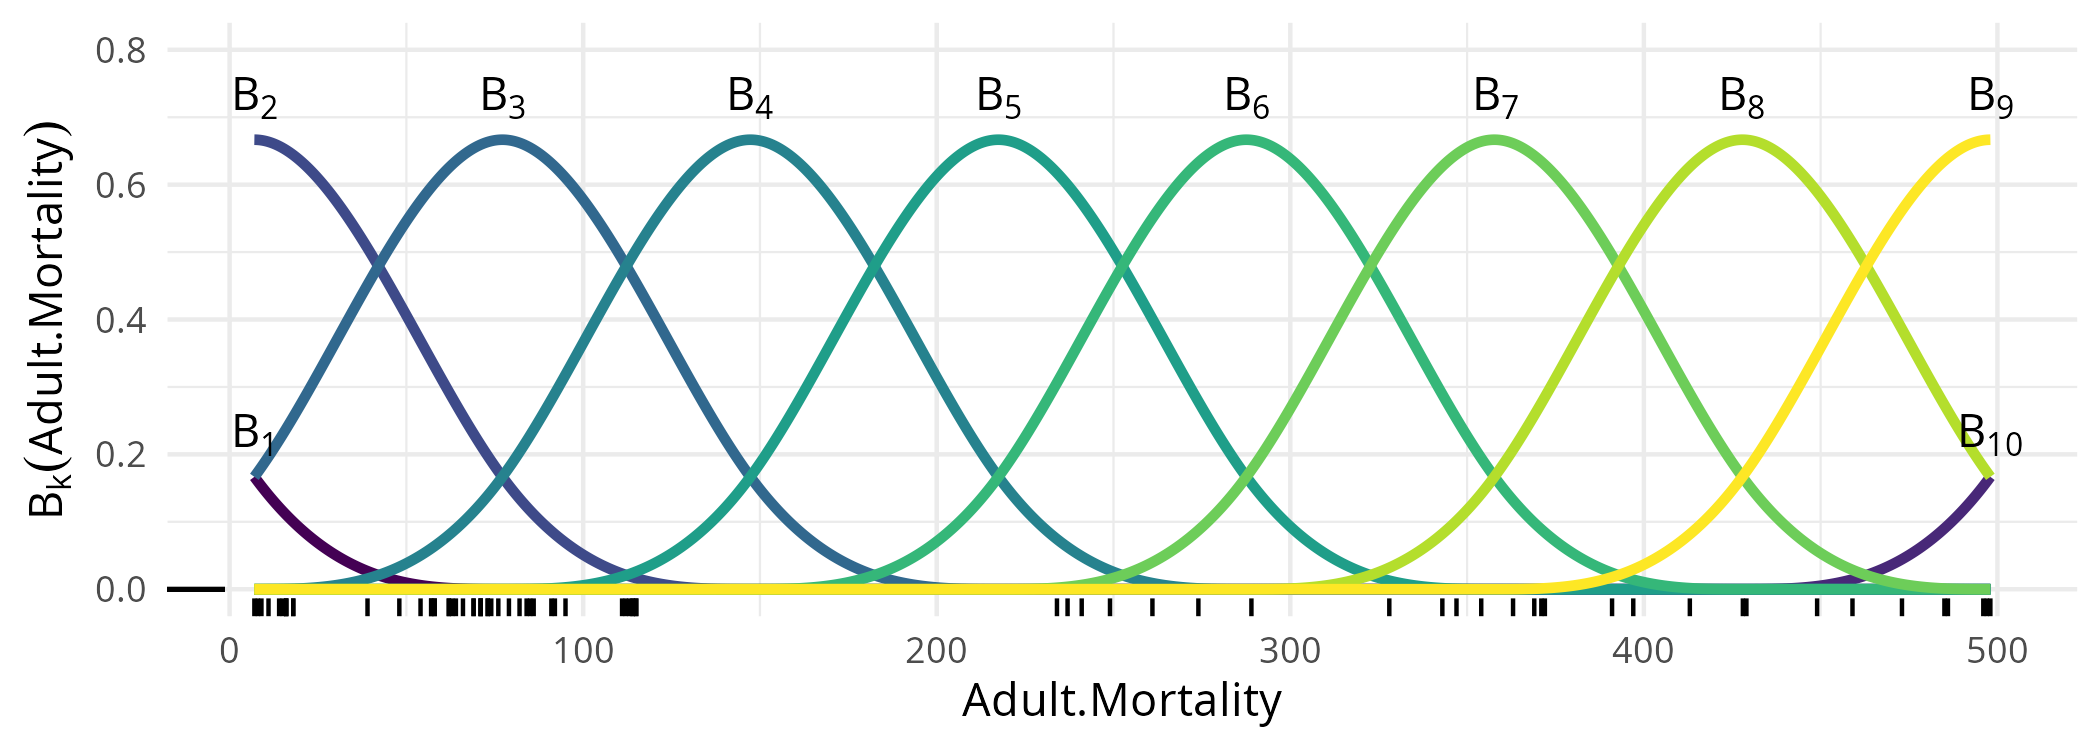
\includegraphics[width=0.7\textwidth]{figures/bs-base/fig-bs0.png}
    \end{figure}

    $$
    \design_k = \left(\begin{array}{c}
      g_{k}^\tran(\xi[1]) \\
      \vdots \\
      g_{k}^\tran(\xi[n])
    \end{array}\right) = \left(\begin{array}{ccc}
      B_{k,1}(\xi[1]) & \dots & B_{k,d_k}(\xi[1]) \\
      \vdots &  & \vdots \\
      B_{k,1}(\xi[n]) & \dots & B_{k,d_k}(\xi[n])
    \end{array}\right)\in\R^{n\times d_k}
    $$
  \end{center}

\end{frame}


\begin{frame}{B/P-spline base learner}
  \vspace{-0.3cm}\[g_k(x) = (B_{k,1}(x), \dots, B_{k,d_k}(x))^\tran\] B-spline basis $B$ of a pre-defined degree~\citep{eilers1996flexible}.
  \begin{center}
    \begin{figure}
      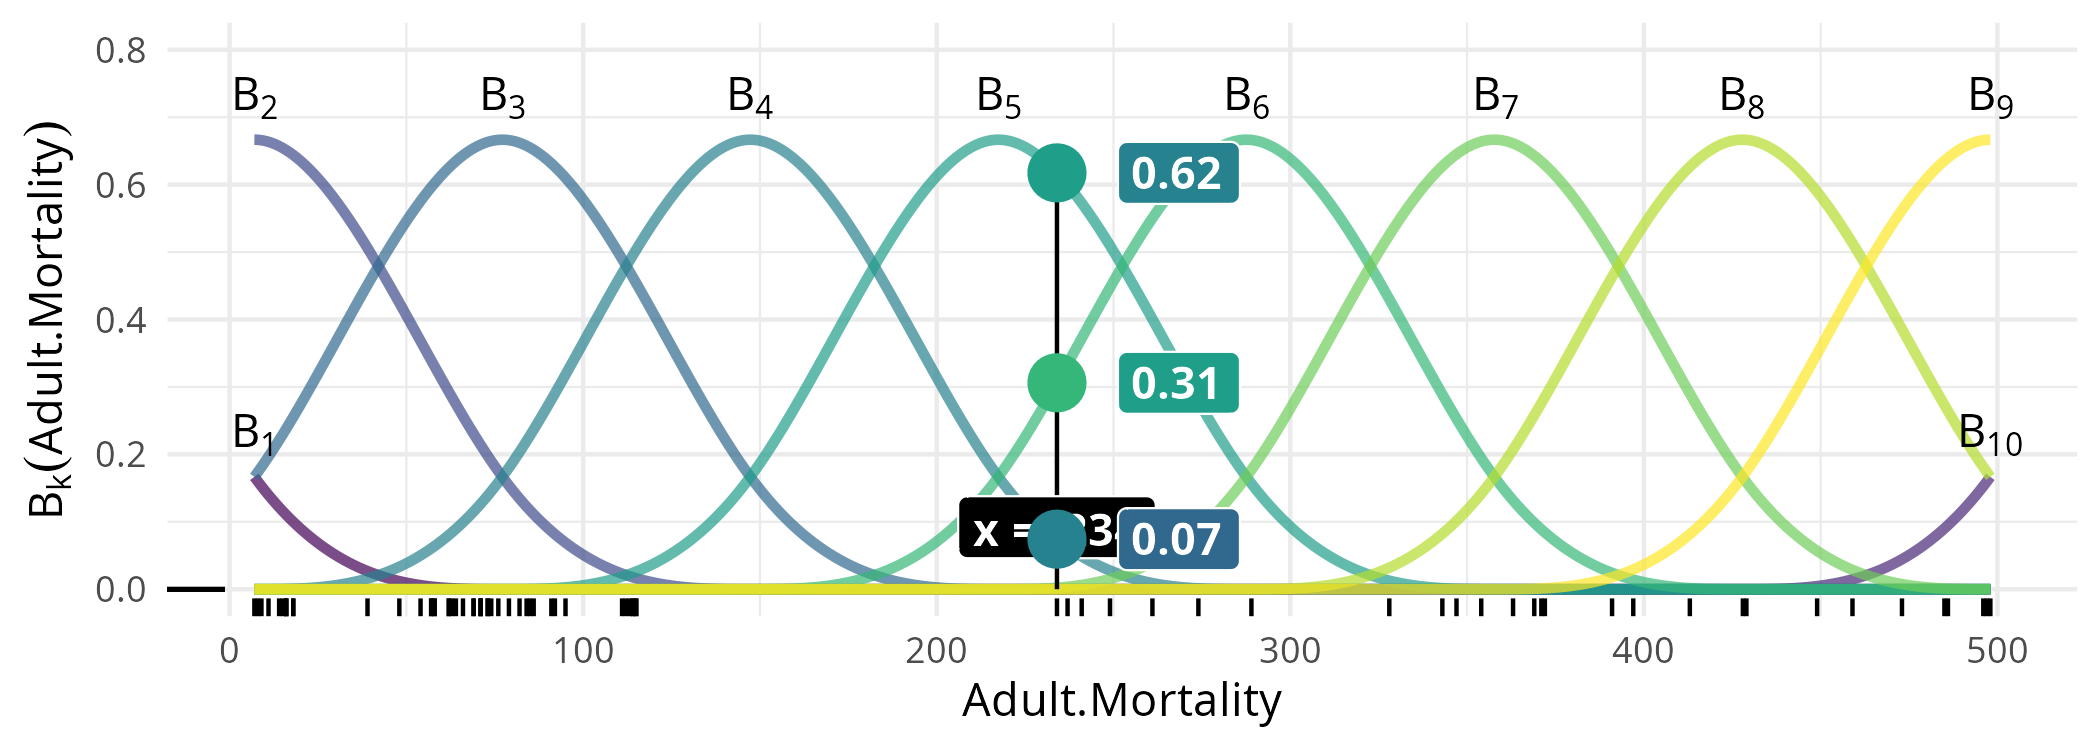
\includegraphics[width=0.7\textwidth]{figures/bs-base/fig-bs1.png}
    \end{figure}
  \end{center}
  \vspace{-0.3cm}
  
\[
\design_k = \tiny\begin{blockarray}{cccccccccc}
\color[HTML]{440154}B_{1} & \color[HTML]{482878}B_{2} & \color[HTML]{3E4A89}B_{3} & \color[HTML]{31688E}B_{4} & \color[HTML]{26828E}B_{5} & \color[HTML]{1F9E89}B_{6} & \color[HTML]{35B779}B_{7} & \color[HTML]{6DCD59}B_{8} & \color[HTML]{B4DE2C}B_{9} & \color[HTML]{FDE725}B_{10} \\
\begin{block}{(cccccccccc)}
\phantom{x}\\
\color{lightgray}0.00 & \color{lightgray}0.00 & \color{lightgray}0.00 & \color[HTML]{31688E}0.07 & \color[HTML]{26828E}0.62 & \color[HTML]{1F9E89}0.31 & \color{lightgray}0.00 & \color{lightgray}0.00 & \color{lightgray}0.00 & \color{lightgray}0.00\color{black}\\
\end{block}
\color{white}0.00 & \color{white}0.20 & \color{white}0.66 & \color{white}0.14 & \color{white}0.00 & \color{white}0.00 & \color{white}0.00 & \color{white}0.00 & \color{white}0.00 & \color{white}0.00\color{black}\\
  \color{white}0.00 & \color{white}0.00 & \color{white}0.00 & \color{white}0.00 & \color{white}0.00 & \color{white}0.00 & \color{white}0.00 & \color{white}0.17 & \color{white}0.67 & \color{white}0.17\color{black}\\
  \color{white}\vdots & \color{white}\vdots & \color{white}\vdots & \color{white}\vdots & \color{white}\vdots & \color{white}\vdots & \color{white}\vdots & \color{white}\vdots & \color{white}\vdots & \color{white}\vdots\\
  \color{white}0.00 & \color{white}0.02 & \color{white}0.48 & \color{white}0.48 & \color{white}0.02 & \color{white}0.00 & \color{white}0.00 & \color{white}0.00 & \color{white}0.00 & \color{white}0.00\color{black}\\
  \color{white}0.00 & \color{white}0.00 & \color{white}0.00 & \color{white}0.01 & \color{white}0.40 & \color{white}0.55 & \color{white}0.04 & \color{white}0.00 & \color{white}0.00 & \color{white}0.00\color{black}\\
  \color{white}0.00 & \color{white}0.00 & \color{white}0.00 & \color{white}0.00 & \color{white}0.00 & \color{white}0.29 & \color{white}0.63 & \color{white}0.08 & \color{white}0.00 & \color{white}0.00\color{black}\\
\phantom{x}
\end{blockarray}
\]
\normalsize

  
\end{frame}


\begin{frame}{B/P-spline base learner}
  \vspace{-0.3cm}\[g_k(x) = (B_{k,1}(x), \dots, B_{k,d_k}(x))^\tran\] B-spline basis $B$ of a pre-defined degree~\citep{eilers1996flexible}.
  \begin{center}
    \begin{figure}
      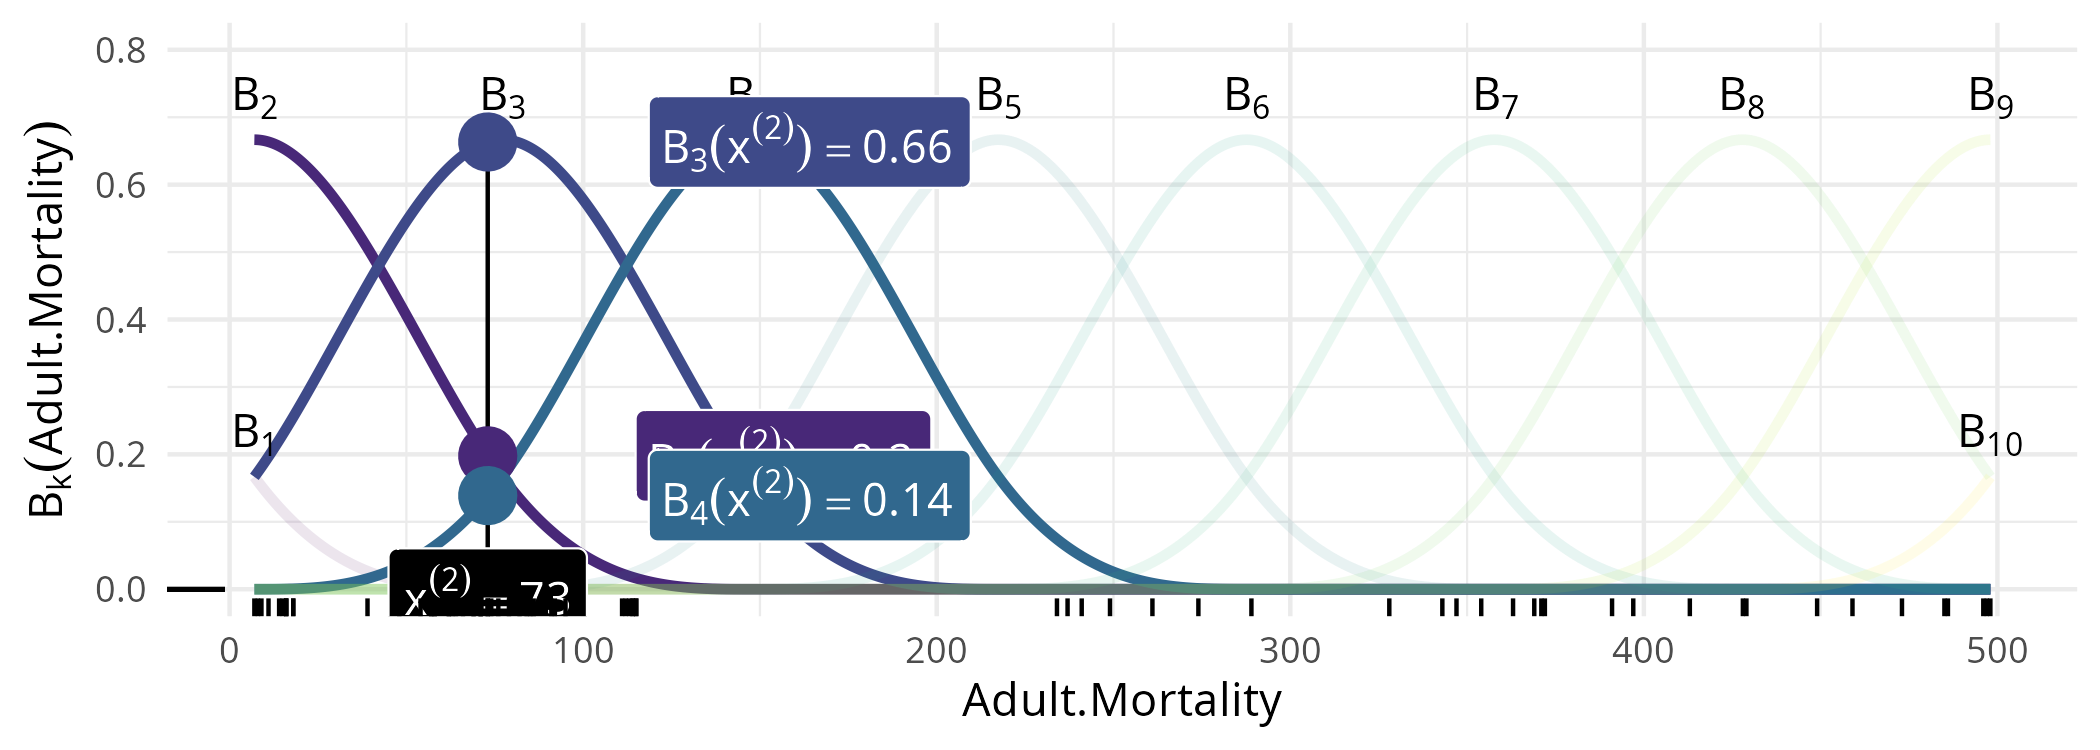
\includegraphics[width=0.7\textwidth]{figures/bs-base/fig-bs59.png}
    \end{figure}
  \end{center}
  \vspace{-0.3cm}
  \[
\design_k = \tiny\begin{blockarray}{cccccccccc}
\color[HTML]{440154}B_{1} & \color[HTML]{482878}B_{2} & \color[HTML]{3E4A89}B_{3} & \color[HTML]{31688E}B_{4} & \color[HTML]{26828E}B_{5} & \color[HTML]{1F9E89}B_{6} & \color[HTML]{35B779}B_{7} & \color[HTML]{6DCD59}B_{8} & \color[HTML]{B4DE2C}B_{9} & \color[HTML]{FDE725}B_{10} \\
\begin{block}{(cccccccccc)}
\phantom{x}\\
\color{lightgray}0.00 & \color{lightgray}0.00 & \color{lightgray}0.00 & \color{gray}0.07 & \color{gray}0.62 & \color{gray}0.31 & \color{lightgray}0.00 & \color{lightgray}0.00 & \color{lightgray}0.00 & \color{lightgray}0.00\color{black}\\
  \color{lightgray}0.00 & \color[HTML]{482878}0.20 & \color[HTML]{3E4A89}0.66 & \color[HTML]{31688E}0.14 & \color{lightgray}0.00 & \color{lightgray}0.00 & \color{lightgray}0.00 & \color{lightgray}0.00 & \color{lightgray}0.00 & \color{lightgray}0.00\color{black}\\
\color{white}0.00 & \color{white}0.00 & \color{white}0.00 & \color{white}0.00 & \color{white}0.00 & \color{white}0.00 & \color{white}0.00 & \color{white}0.17 & \color{white}0.67 & \color{white}0.17\color{black}\\
  \color{white}\vdots & \color{white}\vdots & \color{white}\vdots & \color{white}\vdots & \color{white}\vdots & \color{white}\vdots & \color{white}\vdots & \color{white}\vdots & \color{white}\vdots & \color{white}\vdots\\
  \color{white}0.00 & \color{white}0.02 & \color{white}0.48 & \color{white}0.48 & \color{white}0.02 & \color{white}0.00 & \color{white}0.00 & \color{white}0.00 & \color{white}0.00 & \color{white}0.00\color{black}\\
  \color{white}0.00 & \color{white}0.00 & \color{white}0.00 & \color{white}0.01 & \color{white}0.40 & \color{white}0.55 & \color{white}0.04 & \color{white}0.00 & \color{white}0.00 & \color{white}0.00\color{black}\\
  \color{white}0.00 & \color{white}0.00 & \color{white}0.00 & \color{white}0.00 & \color{white}0.00 & \color{white}0.29 & \color{white}0.63 & \color{white}0.08 & \color{white}0.00 & \color{white}0.00\color{black}\\
\phantom{x}\\
\end{block}
\end{blockarray}
\]
\normalsize

  \addtocounter{framenumber}{-1}
\end{frame}


\begin{frame}{B/P-spline base learner}
  \vspace{-0.3cm}\[g_k(x) = (B_{k,1}(x), \dots, B_{k,d_k}(x))^\tran\] B-spline basis $B$ of a pre-defined degree~\citep{eilers1996flexible}.
  \begin{center}
    \begin{figure}
      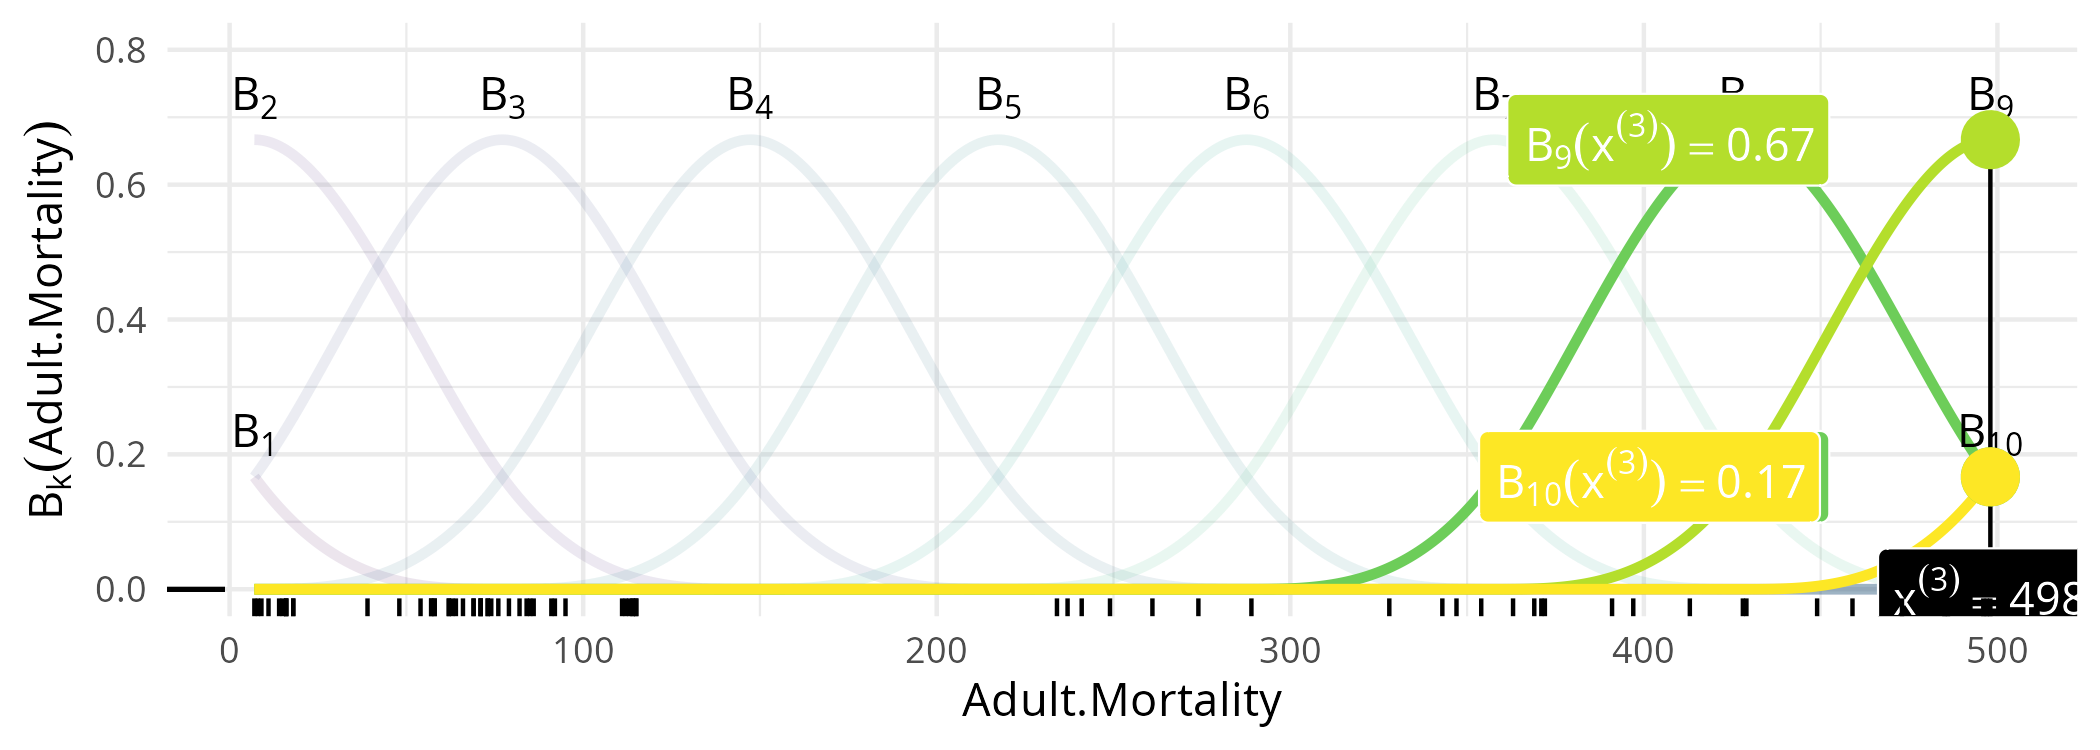
\includegraphics[width=0.7\textwidth]{figures/bs-base/fig-bs40.png}
    \end{figure}
  \end{center}
  \vspace{-0.3cm}
  \scriptsize
$$
\design_k = \begin{blockarray}{cccccccccc}
\color[HTML]{440154}B_{1} & \color[HTML]{482878}B_{2} & \color[HTML]{3E4A89}B_{3} & \color[HTML]{31688E}B_{4} & \color[HTML]{26828E}B_{5} & \color[HTML]{1F9E89}B_{6} & \color[HTML]{35B779}B_{7} & \color[HTML]{6DCD59}B_{8} & \color[HTML]{B4DE2C}B_{9} & \color[HTML]{FDE725}B_{10} \\
\begin{block}{(cccccccccc)}
\color{lightgray}0.00 & \color{lightgray}0.00 & \color{lightgray}0.00 & \color{gray}0.07 & \color{gray}0.62 & \color{gray}0.31 & \color{lightgray}0.00 & \color{lightgray}0.00 & \color{lightgray}0.00 & \color{lightgray}0.00\color{black}\\
  \color{lightgray}0.00 & \color{gray}0.20 & \color{gray}0.66 & \color{gray}0.14 & \color{lightgray}0.00 & \color{lightgray}0.00 & \color{lightgray}0.00 & \color{lightgray}0.00 & \color{lightgray}0.00 & \color{lightgray}0.00\color{black}\\
  \color{lightgray}0.00 & \color{lightgray}0.00 & \color{lightgray}0.00 & \color{lightgray}0.00 & \color{lightgray}0.00 & \color{lightgray}0.00 & \color{lightgray}0.00 & \color[HTML]{6DCD59}0.17 & \color[HTML]{B4DE2C}0.67 & \color[HTML]{FDE725}0.17\color{black}\\
  \color{white}\vdots & \color{white}\vdots & \color{white}\vdots & \color{white}\vdots & \color{white}\vdots & \color{white}\vdots & \color{white}\vdots & \color{white}\vdots & \color{white}\vdots & \color{white}\vdots\\
  
\end{block}
\color{white}0.00 & \color{white}0.02 & \color{white}0.48 & \color{white}0.48 & \color{white}0.02 & \color{white}0.00 & \color{white}0.00 & \color{white}0.00 & \color{white}0.00 & \color{white}0.00\color{black}\\
  \color{white}0.00 & \color{white}0.00 & \color{white}0.00 & \color{white}0.01 & \color{white}0.40 & \color{white}0.55 & \color{white}0.04 & \color{white}0.00 & \color{white}0.00 & \color{white}0.00\color{black}\\
  \color{white}0.00 & \color{white}0.00 & \color{white}0.00 & \color{white}0.00 & \color{white}0.00 & \color{white}0.29 & \color{white}0.63 & \color{white}0.08 & \color{white}0.00 & \color{white}0.00\color{black}
\end{blockarray}
$$
\normalsize

  \addtocounter{framenumber}{-1}
\end{frame}


\begin{frame}{B/P-spline base learner}
  \vspace{-0.3cm}\[g_k(x) = (B_{k,1}(x), \dots, B_{k,d_k}(x))^\tran\] B-spline basis $B$ of a pre-defined degree~\citep{eilers1996flexible}.
  \begin{center}
    \begin{figure}
      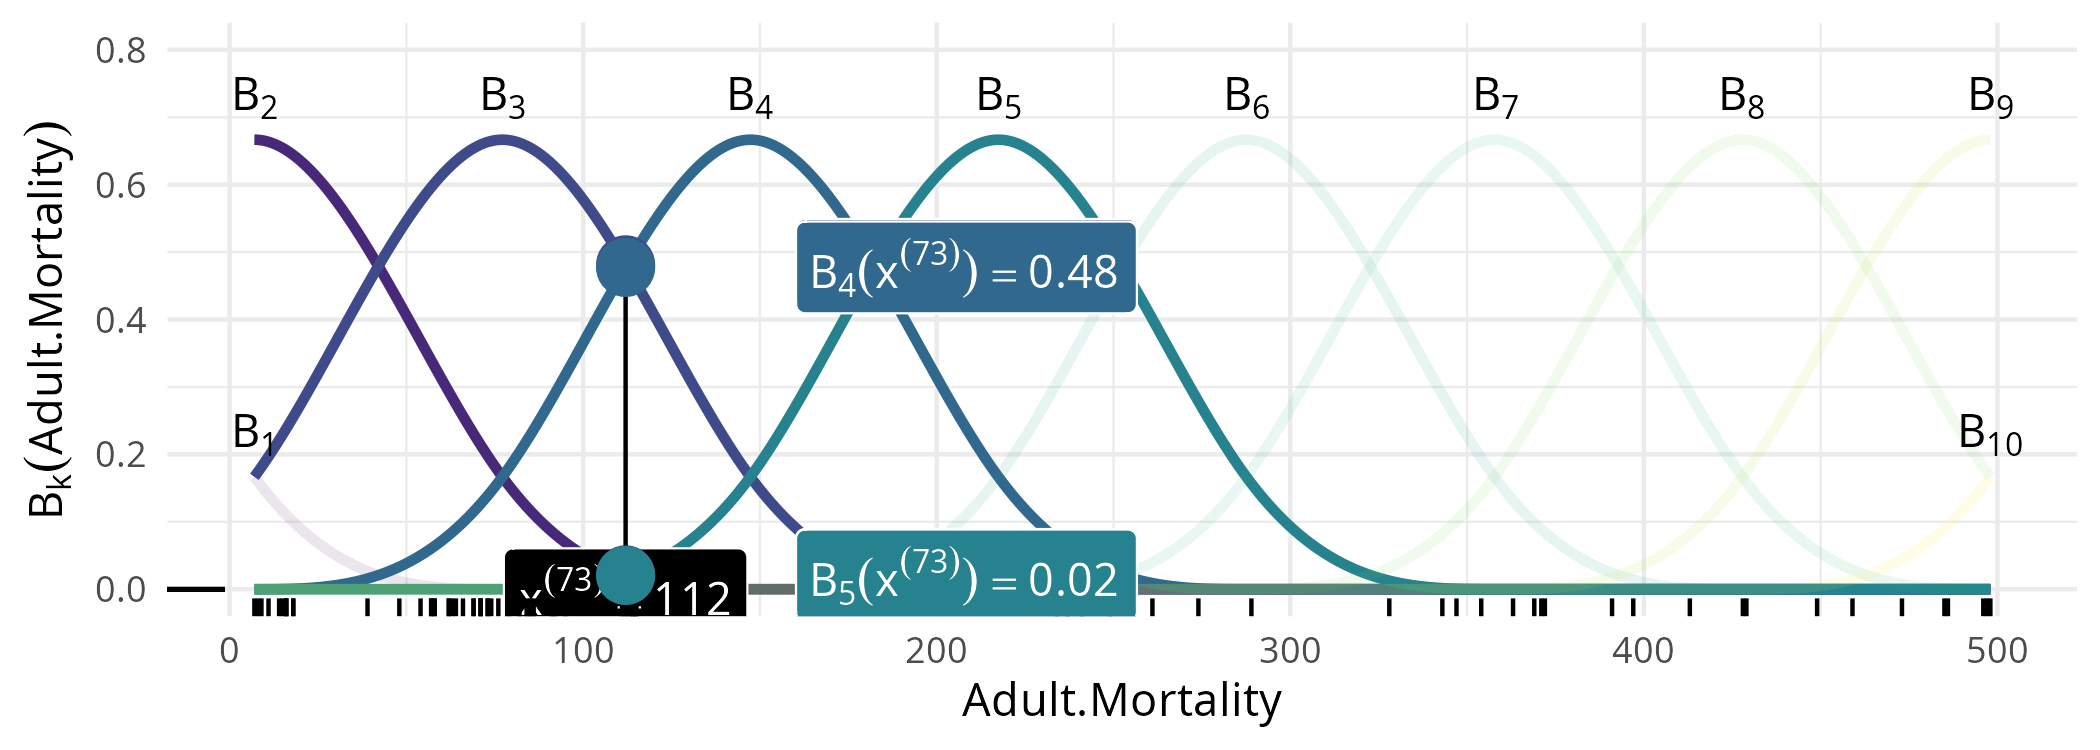
\includegraphics[width=0.7\textwidth]{figures/bs-base/fig-bs70.png}
    \end{figure}
  \end{center}
  \vspace{-0.3cm}
  \[
\design_k = \tiny\begin{blockarray}{cccccccccc}
\color[HTML]{440154}B_{1} & \color[HTML]{482878}B_{2} & \color[HTML]{3E4A89}B_{3} & \color[HTML]{31688E}B_{4} & \color[HTML]{26828E}B_{5} & \color[HTML]{1F9E89}B_{6} & \color[HTML]{35B779}B_{7} & \color[HTML]{6DCD59}B_{8} & \color[HTML]{B4DE2C}B_{9} & \color[HTML]{FDE725}B_{10} \\
\begin{block}{(cccccccccc)}
\phantom{x}\\
\color{lightgray}0.00 & \color{lightgray}0.00 & \color{lightgray}0.00 & \color{gray}0.07 & \color{gray}0.62 & \color{gray}0.31 & \color{lightgray}0.00 & \color{lightgray}0.00 & \color{lightgray}0.00 & \color{lightgray}0.00\color{black}\\
  \color{lightgray}0.00 & \color{gray}0.20 & \color{gray}0.66 & \color{gray}0.14 & \color{lightgray}0.00 & \color{lightgray}0.00 & \color{lightgray}0.00 & \color{lightgray}0.00 & \color{lightgray}0.00 & \color{lightgray}0.00\color{black}\\
  \color{lightgray}0.00 & \color{lightgray}0.00 & \color{lightgray}0.00 & \color{lightgray}0.00 & \color{lightgray}0.00 & \color{lightgray}0.00 & \color{lightgray}0.00 & \color{gray}0.17 & \color{gray}0.67 & \color{gray}0.17\color{black}\\
  \color{black}\vdots & \color{black}\vdots & \color{black}\vdots & \color{black}\vdots & \color{black}\vdots & \color{black}\vdots & \color{black}\vdots & \color{black}\vdots & \color{black}\vdots & \color{black}\vdots\\
  \color{lightgray}0.00 & \color[HTML]{482878}0.02 & \color[HTML]{3E4A89}0.48 & \color[HTML]{31688E}0.48 & \color[HTML]{26828E}0.02 & \color{lightgray}0.00 & \color{lightgray}0.00 & \color{lightgray}0.00 & \color{lightgray}0.00 & \color{lightgray}0.00\color{black}\\
\color{white}0.00 & \color{white}0.00 & \color{white}0.00 & \color{white}0.01 & \color{white}0.40 & \color{white}0.55 & \color{white}0.04 & \color{white}0.00 & \color{white}0.00 & \color{white}0.00\color{black}\\
  \color{white}0.00 & \color{white}0.00 & \color{white}0.00 & \color{white}0.00 & \color{white}0.00 & \color{white}0.29 & \color{white}0.63 & \color{white}0.08 & \color{white}0.00 & \color{white}0.00\color{black}\\
\phantom{x}\\
\end{block}
\end{blockarray}
\]
\normalsize

  \addtocounter{framenumber}{-1}
\end{frame}


\begin{frame}{B/P-spline base learner}
  \vspace{-0.3cm}\[g_k(x) = (B_{k,1}(x), \dots, B_{k,d_k}(x))^\tran\] B-spline basis $B$ of a pre-defined degree~\citep{eilers1996flexible}.
  \begin{center}
    \begin{figure}
      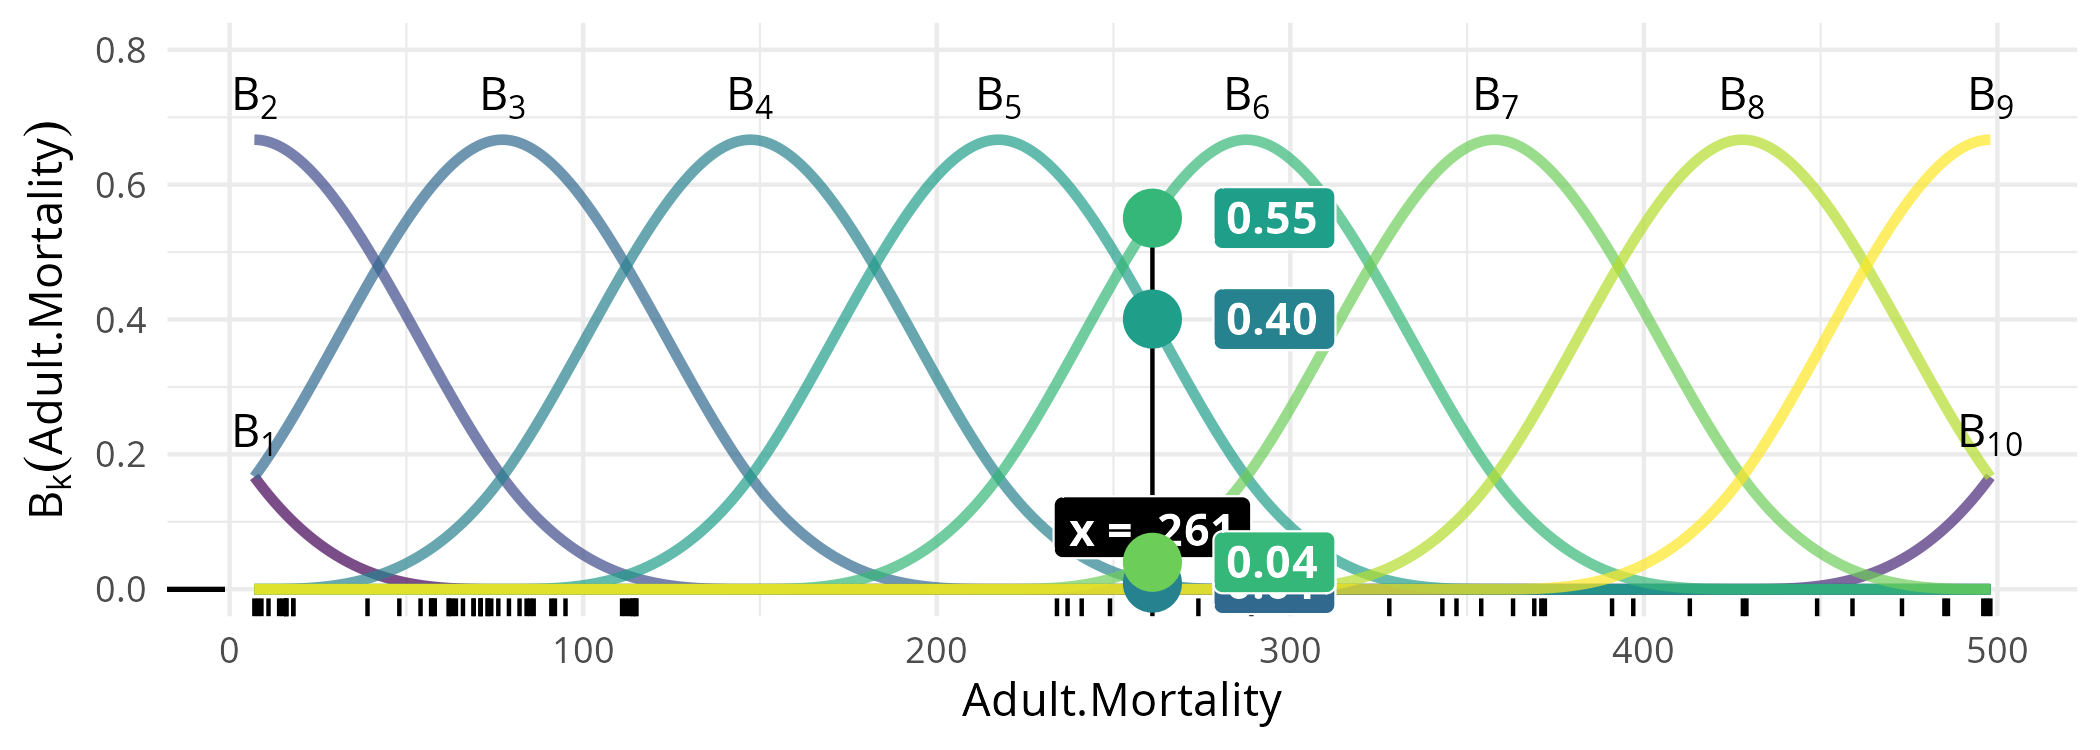
\includegraphics[width=0.7\textwidth]{figures/bs-base/fig-bs5.png}
    \end{figure}
  \end{center}
  \vspace{-0.3cm}
  \[
\design_k = \tiny\begin{blockarray}{cccccccccc}
\color[HTML]{440154}B_{1} & \color[HTML]{482878}B_{2} & \color[HTML]{3E4A89}B_{3} & \color[HTML]{31688E}B_{4} & \color[HTML]{26828E}B_{5} & \color[HTML]{1F9E89}B_{6} & \color[HTML]{35B779}B_{7} & \color[HTML]{6DCD59}B_{8} & \color[HTML]{B4DE2C}B_{9} & \color[HTML]{FDE725}B_{10} \\
\begin{block}{(cccccccccc)}
\phantom{x}\\
\color{lightgray}0.00 & \color{lightgray}0.00 & \color{lightgray}0.00 & \color{gray}0.07 & \color{gray}0.62 & \color{gray}0.31 & \color{lightgray}0.00 & \color{lightgray}0.00 & \color{lightgray}0.00 & \color{lightgray}0.00\color{black}\\
  \color{lightgray}0.00 & \color{gray}0.20 & \color{gray}0.66 & \color{gray}0.14 & \color{lightgray}0.00 & \color{lightgray}0.00 & \color{lightgray}0.00 & \color{lightgray}0.00 & \color{lightgray}0.00 & \color{lightgray}0.00\color{black}\\
  \color{lightgray}0.00 & \color{lightgray}0.00 & \color{lightgray}0.00 & \color{lightgray}0.00 & \color{lightgray}0.00 & \color{lightgray}0.00 & \color{lightgray}0.00 & \color{gray}0.17 & \color{gray}0.67 & \color{gray}0.17\color{black}\\
  \color{black}\vdots & \color{black}\vdots & \color{black}\vdots & \color{black}\vdots & \color{black}\vdots & \color{black}\vdots & \color{black}\vdots & \color{black}\vdots & \color{black}\vdots & \color{black}\vdots\\
  \color{lightgray}0.00 & \color{gray}0.02 & \color{gray}0.48 & \color{gray}0.48 & \color{gray}0.02 & \color{lightgray}0.00 & \color{lightgray}0.00 & \color{lightgray}0.00 & \color{lightgray}0.00 & \color{lightgray}0.00\color{black}\\
  \color{lightgray}0.00 & \color{lightgray}0.00 & \color{lightgray}0.00 & \color[HTML]{31688E}0.01 & \color[HTML]{26828E}0.40 & \color[HTML]{1F9E89}0.55 & \color[HTML]{35B779}0.04 & \color{lightgray}0.00 & \color{lightgray}0.00 & \color{lightgray}0.00\color{black}\\
\color{white}0.00 & \color{white}0.00 & \color{white}0.00 & \color{white}0.00 & \color{white}0.00 & \color{white}0.29 & \color{white}0.63 & \color{white}0.08 & \color{white}0.00 & \color{white}0.00\color{black}\\
\phantom{x}\\
\end{block}
\end{blockarray}
\]
\normalsize

  \addtocounter{framenumber}{-1}
\end{frame}


\begin{frame}{B/P-spline base learner}
  \vspace{-0.3cm}\[g_k(x) = (B_{k,1}(x), \dots, B_{k,d_k}(x))^\tran\] B-spline basis $B$ of a pre-defined degree~\citep{eilers1996flexible}.
  \begin{center}
    \begin{figure}
      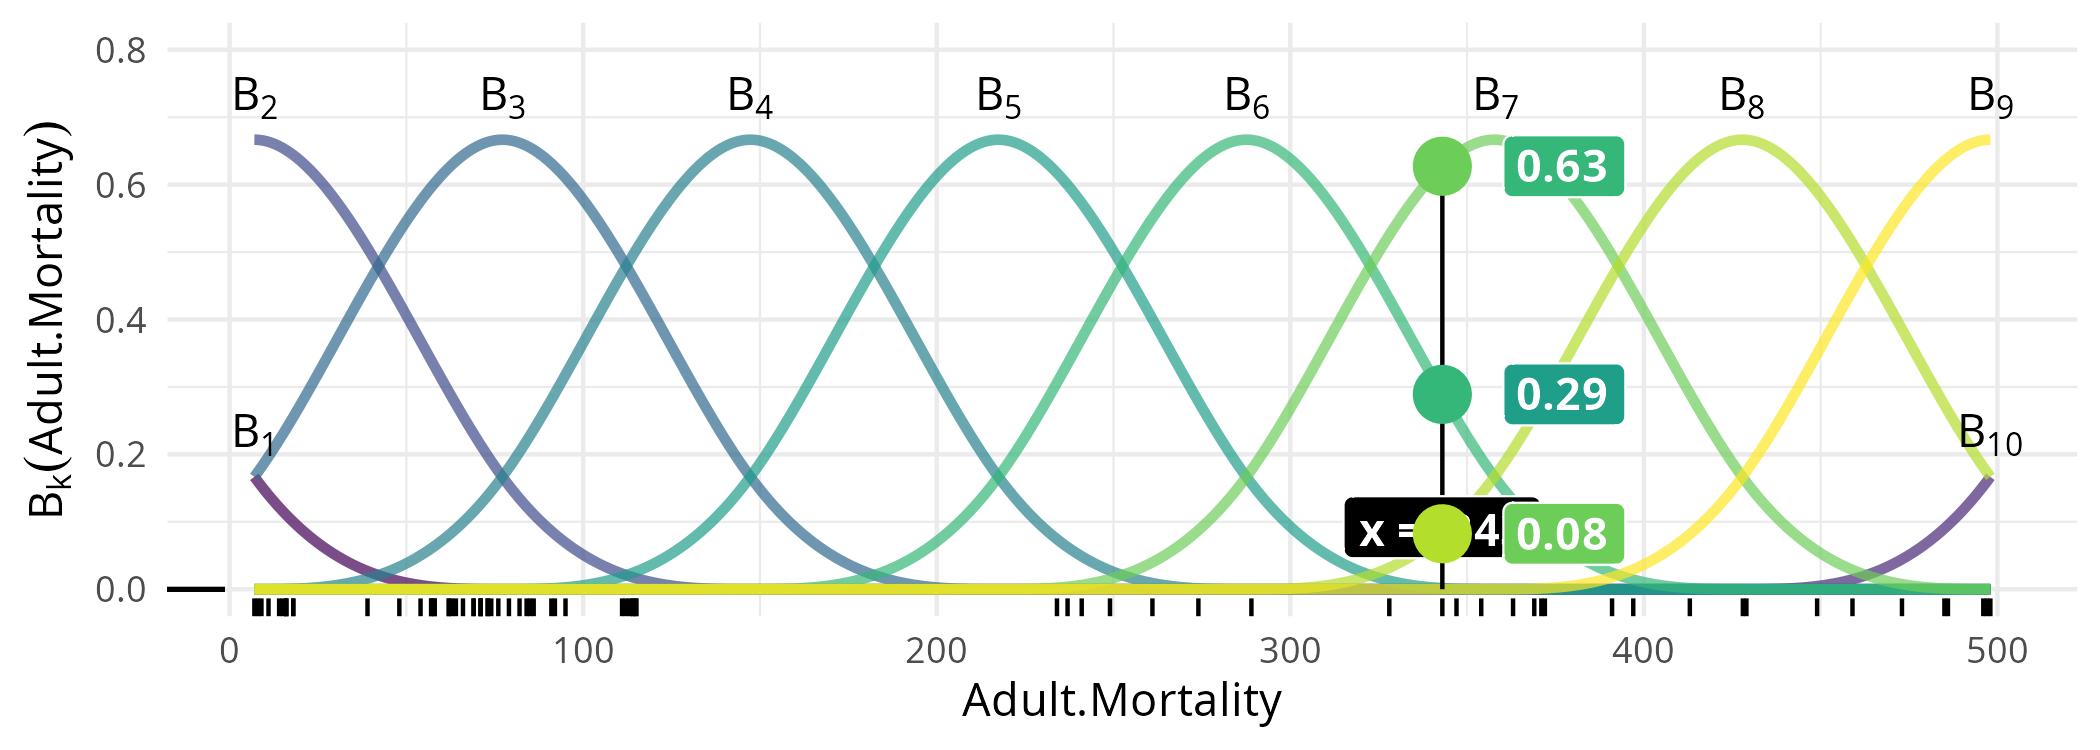
\includegraphics[width=0.7\textwidth]{figures/bs-base/fig-bs10.png}
    \end{figure}
  \end{center}
  \vspace{-0.3cm}
  \[
\design_k = \tiny\begin{blockarray}{cccccccccc}
\color[HTML]{440154}B_{1} & \color[HTML]{482878}B_{2} & \color[HTML]{3E4A89}B_{3} & \color[HTML]{31688E}B_{4} & \color[HTML]{26828E}B_{5} & \color[HTML]{1F9E89}B_{6} & \color[HTML]{35B779}B_{7} & \color[HTML]{6DCD59}B_{8} & \color[HTML]{B4DE2C}B_{9} & \color[HTML]{FDE725}B_{10} \\
\begin{block}{(cccccccccc)}
\phantom{x}\\
\color{lightgray}0.00 & \color{lightgray}0.00 & \color{lightgray}0.00 & \color{gray}0.07 & \color{gray}0.62 & \color{gray}0.31 & \color{lightgray}0.00 & \color{lightgray}0.00 & \color{lightgray}0.00 & \color{lightgray}0.00\color{black}\\
  \color{lightgray}0.00 & \color{gray}0.20 & \color{gray}0.66 & \color{gray}0.14 & \color{lightgray}0.00 & \color{lightgray}0.00 & \color{lightgray}0.00 & \color{lightgray}0.00 & \color{lightgray}0.00 & \color{lightgray}0.00\color{black}\\
  \color{lightgray}0.00 & \color{lightgray}0.00 & \color{lightgray}0.00 & \color{lightgray}0.00 & \color{lightgray}0.00 & \color{lightgray}0.00 & \color{lightgray}0.00 & \color{gray}0.17 & \color{gray}0.67 & \color{gray}0.17\color{black}\\
  \color{black}\vdots & \color{black}\vdots & \color{black}\vdots & \color{black}\vdots & \color{black}\vdots & \color{black}\vdots & \color{black}\vdots & \color{black}\vdots & \color{black}\vdots & \color{black}\vdots\\
  \color{lightgray}0.00 & \color{gray}0.02 & \color{gray}0.48 & \color{gray}0.48 & \color{gray}0.02 & \color{lightgray}0.00 & \color{lightgray}0.00 & \color{lightgray}0.00 & \color{lightgray}0.00 & \color{lightgray}0.00\color{black}\\
  \color{lightgray}0.00 & \color{lightgray}0.00 & \color{lightgray}0.00 & \color{gray}0.01 & \color{gray}0.40 & \color{gray}0.55 & \color{gray}0.04 & \color{lightgray}0.00 & \color{lightgray}0.00 & \color{lightgray}0.00\color{black}\\
  \color{lightgray}0.00 & \color{lightgray}0.00 & \color{lightgray}0.00 & \color{lightgray}0.00 & \color{lightgray}0.00 & \color[HTML]{1F9E89}0.29 & \color[HTML]{35B779}0.63 & \color[HTML]{6DCD59}0.08 & \color{lightgray}0.00 & \color{lightgray}0.00\color{black}\\
\phantom{x}\\
\end{block}
\end{blockarray}
\]
\normalsize

  \addtocounter{framenumber}{-1}
\end{frame}



\begin{frame}{Component-wise gradient boosting -- Base learner examples II}
  \textbf{Categorical base learner} $g_k(x) = (g_{k,1}(x), \dots, g_{k,G}(x))^\tran = (\mathds{1}_{\{x = 1\}}, \dots, \mathds{1}_{\{x = G\}})^\tran$ with categorical $x\in\{1, \dots, G\}$.

  \begin{center}
    \begin{figure}
      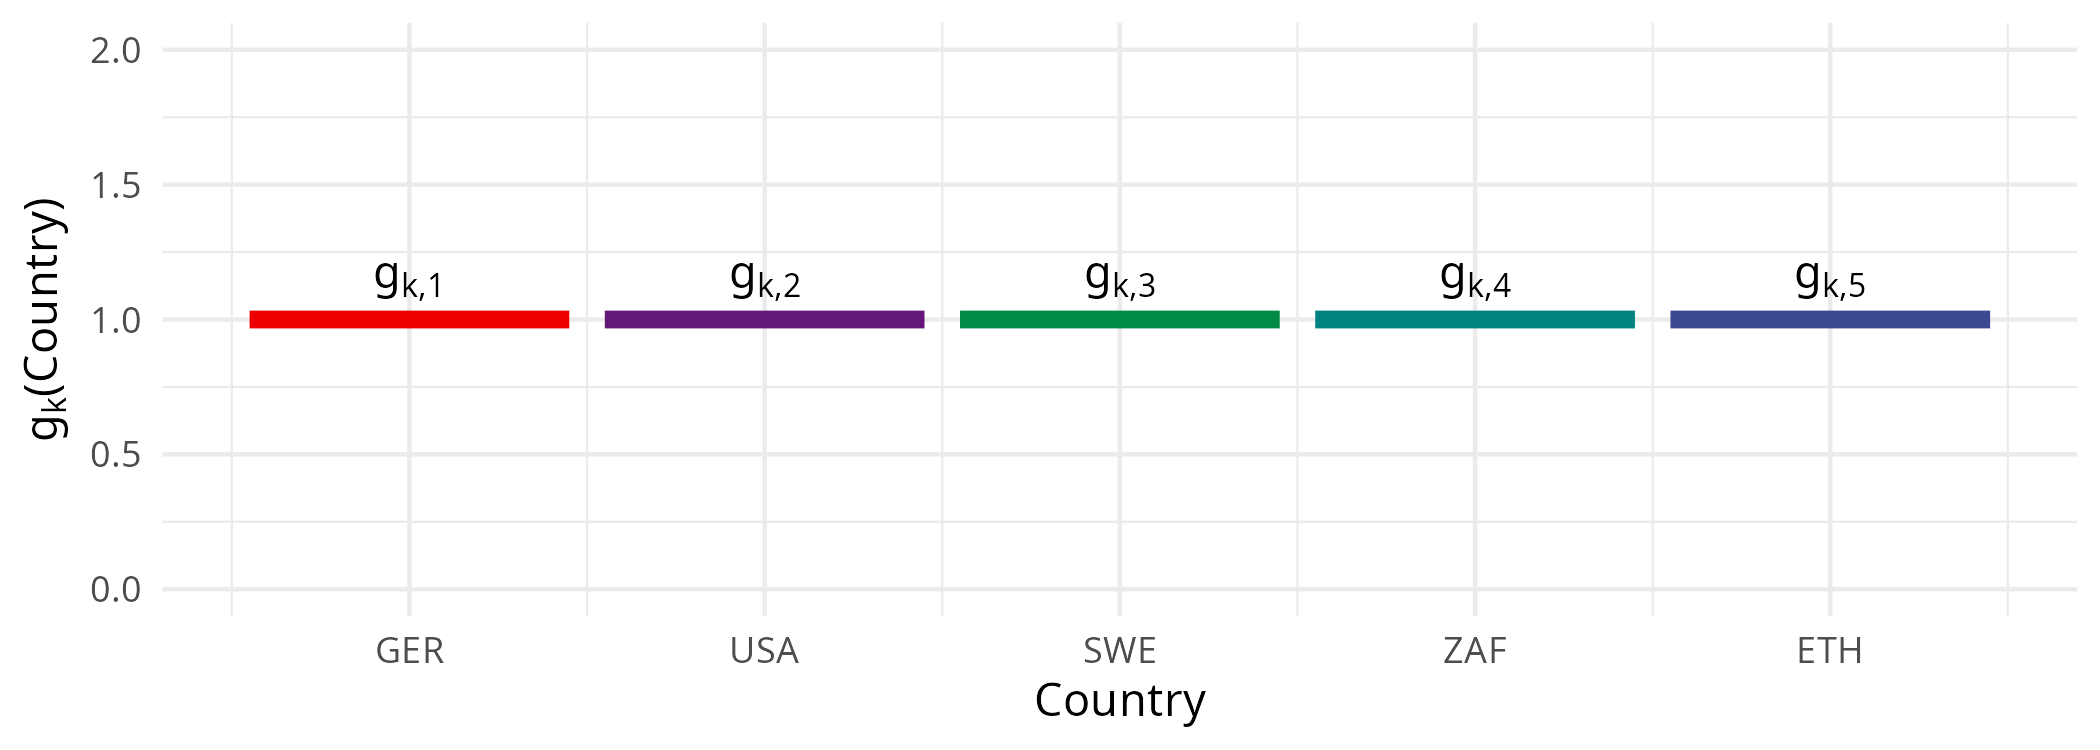
\includegraphics[width=0.7\textwidth]{figures/bs-cat/fig-cat0.png}
    \end{figure}
    \vspace{-0.5cm}
    $$
    \design_k = \left(\begin{array}{c}
      g_{k}^\tran(\xi[1]) \\
      \vdots \\
      g_{k}^\tran(\xi[n])
    \end{array}\right) = \left(\begin{array}{ccc}
      \mathds{1}_{\{\xi[1] = 1\}} & \dots & \mathds{1}_{\{\xi[1] = G\}} \\
      \vdots &  & \vdots \\
      \mathds{1}_{\{\xi[n] = 1\}} & \dots & \mathds{1}_{\{\xi[n] = G\}} \\
    \end{array}\right)\in\R^{n\times G}
    $$
  \end{center}

\end{frame}

\begin{frame}{Component-wise gradient boosting -- Base learner examples II}
  \textbf{Categorical base learner} $g_k(x) = (g_{k,1}(x), \dots, g_{k,G}(x))^\tran = (\mathds{1}_{\{x = 1\}}, \dots, \mathds{1}_{\{x = G\}})^\tran$ with categorical $x\in\{1, \dots, G\}$.

  \begin{center}
    \begin{figure}
      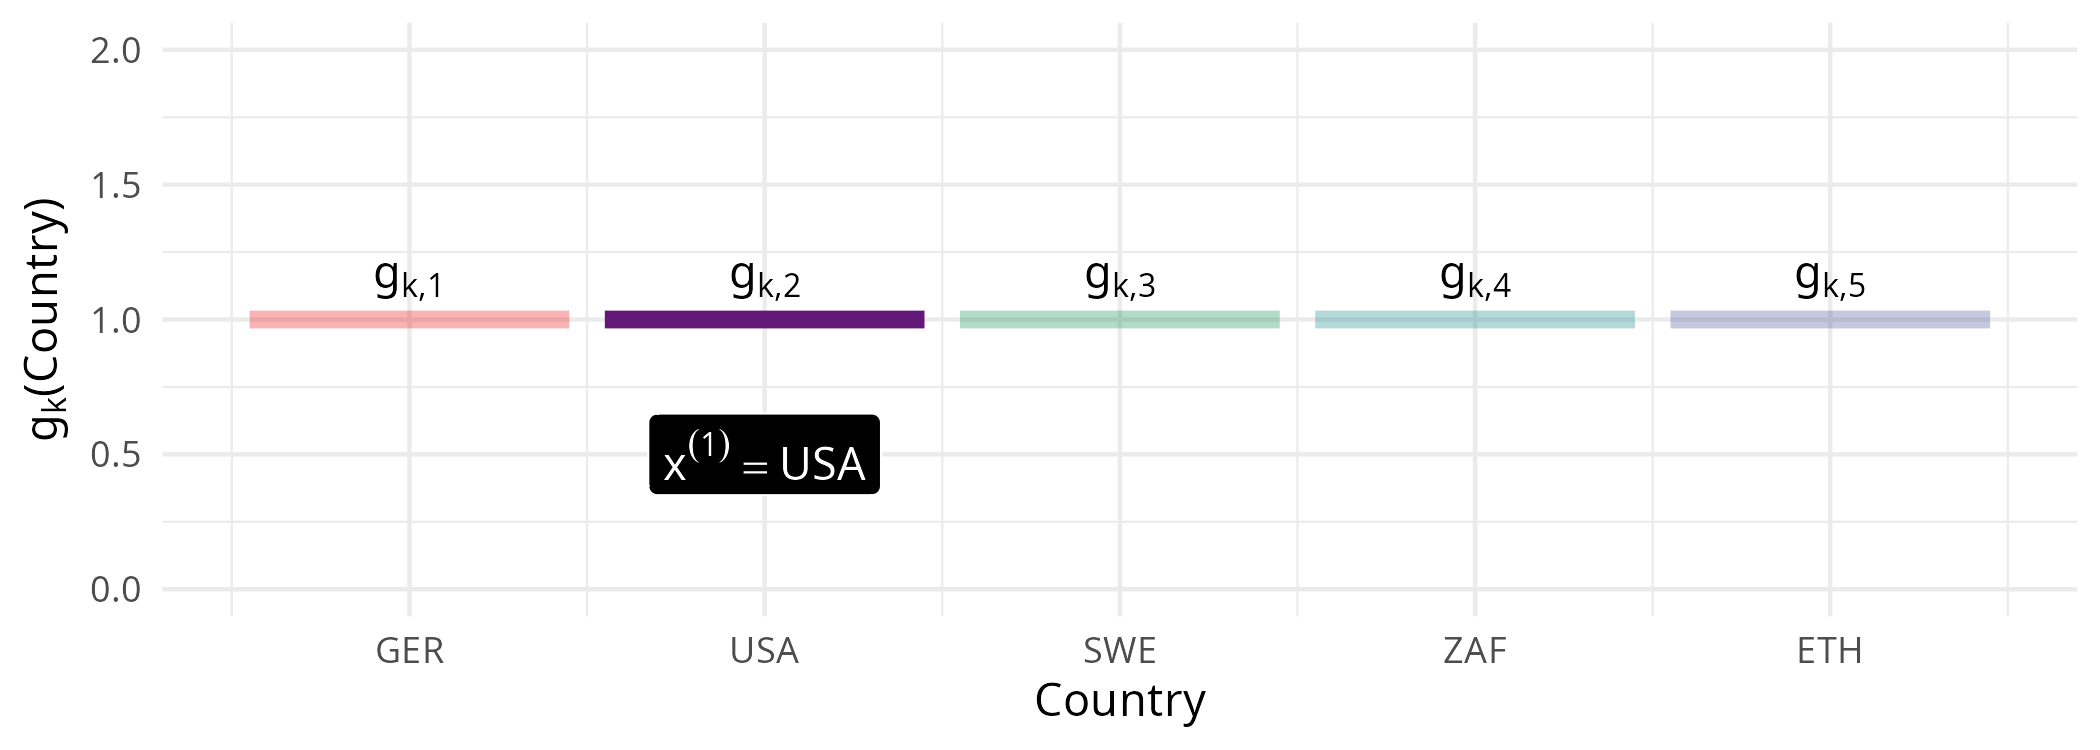
\includegraphics[width=0.7\textwidth]{figures/bs-cat/fig-cat1.png}
    \end{figure}
    \vspace{-0.5cm}
    \scriptsize
    $$
      \design_k = \begin{blockarray}{ccccc}
        \color[HTML]{EE0000}g_{k,GER} & \color[HTML]{631879}g_{k,USA} & \color[HTML]{008B45}g_{k,SWE} & \color[HTML]{008280}g_{k,ZAF} & \color[HTML]{3B4992}g_{k,ETH}\\
      \begin{block}{(ccccc)}
        \color{lightgray}0 & \color[HTML]{631879}\bm{1} & \color{lightgray}0 & \color{lightgray}0 & \color{lightgray}0 \\
      \color{white}0 & \color{white}0 & \color{white}0 & \color{white}0 & \color{white}0 \\
      \color{white}0 & \color{white}0 & \color{white}0 & \color{white}0 & \color{white}0 \\
      \color{white}\vdots & \color{white}\vdots & \color{white}\vdots & \color{white}\vdots & \color{white}\vdots \\
      \color{white}0 & \color{white}0 & \color{white}0 & \color{white}0 & \color{white}0 \\
      \color{white}0 & \color{white}0 & \color{white}0 & \color{white}0 & \color{white}0 \\
      \color{white}0 & \color{white}0 & \color{white}0 & \color{white}0 & \color{white}0 \color{black}\\
      \end{block}
    \end{blockarray}
    $$
    \normalsize
  \end{center}
\end{frame}

\begin{frame}{Component-wise gradient boosting -- Base learner examples II}
  \textbf{Categorical base learner} $g_k(x) = (g_{k,1}(x), \dots, g_{k,G}(x))^\tran = (\mathds{1}_{\{x = 1\}}, \dots, \mathds{1}_{\{x = G\}})^\tran$ with categorical $x\in\{1, \dots, G\}$.

  \begin{center}
    \begin{figure}
      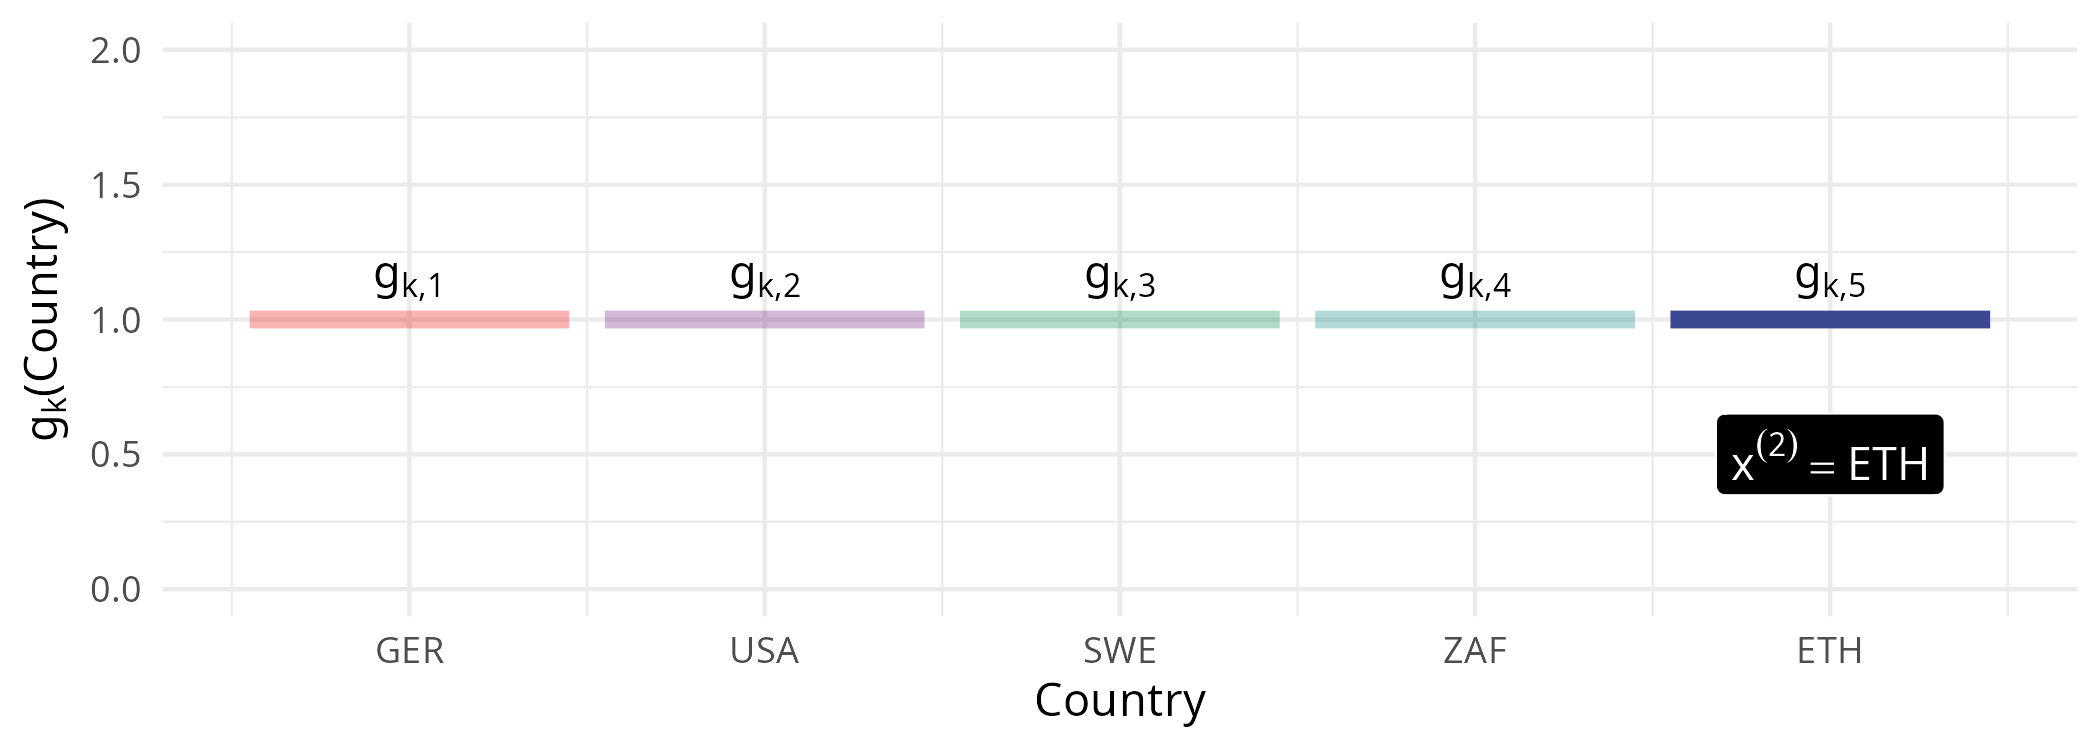
\includegraphics[width=0.7\textwidth]{figures/bs-cat/fig-cat2.png}
    \end{figure}
    \vspace{-0.5cm}
    \scriptsize
    $$
      \design_k = \begin{blockarray}{ccccc}
        \color[HTML]{EE0000}g_{k,GER} & \color[HTML]{631879}g_{k,USA} & \color[HTML]{008B45}g_{k,SWE} & \color[HTML]{008280}g_{k,ZAF} & \color[HTML]{3B4992}g_{k,ETH}\\
      \begin{block}{(ccccc)}
        \color{lightgray}0 & \color{black}\bm{1} & \color{lightgray}0 & \color{lightgray}0 & \color{lightgray}0 \\
      \color{lightgray}0 & \color{lightgray}0 & \color{lightgray}0 & \color{lightgray}0 & \color[HTML]{3B4992}\bm{1} \\
      \color{white}0 & \color{white}0 & \color{white}0 & \color{white}0 & \color{white}0 \\
      \color{white}\vdots & \color{white}\vdots & \color{white}\vdots & \color{white}\vdots & \color{white}\vdots \\
      \color{white}0 & \color{white}0 & \color{white}0 & \color{white}0 & \color{white}0 \\
      \color{white}0 & \color{white}0 & \color{white}0 & \color{white}0 & \color{white}0 \\
      \color{white}0 & \color{white}0 & \color{white}0 & \color{white}0 & \color{white}0 \color{black}\\
      \end{block}
    \end{blockarray}
    $$
    \normalsize
  \end{center}
\end{frame}

\begin{frame}{Component-wise gradient boosting -- Base learner examples II}
  \textbf{Categorical base learner} $g_k(x) = (g_{k,1}(x), \dots, g_{k,G}(x))^\tran = (\mathds{1}_{\{x = 1\}}, \dots, \mathds{1}_{\{x = G\}})^\tran$ with categorical $x\in\{1, \dots, G\}$.

  \begin{center}
    \begin{figure}
      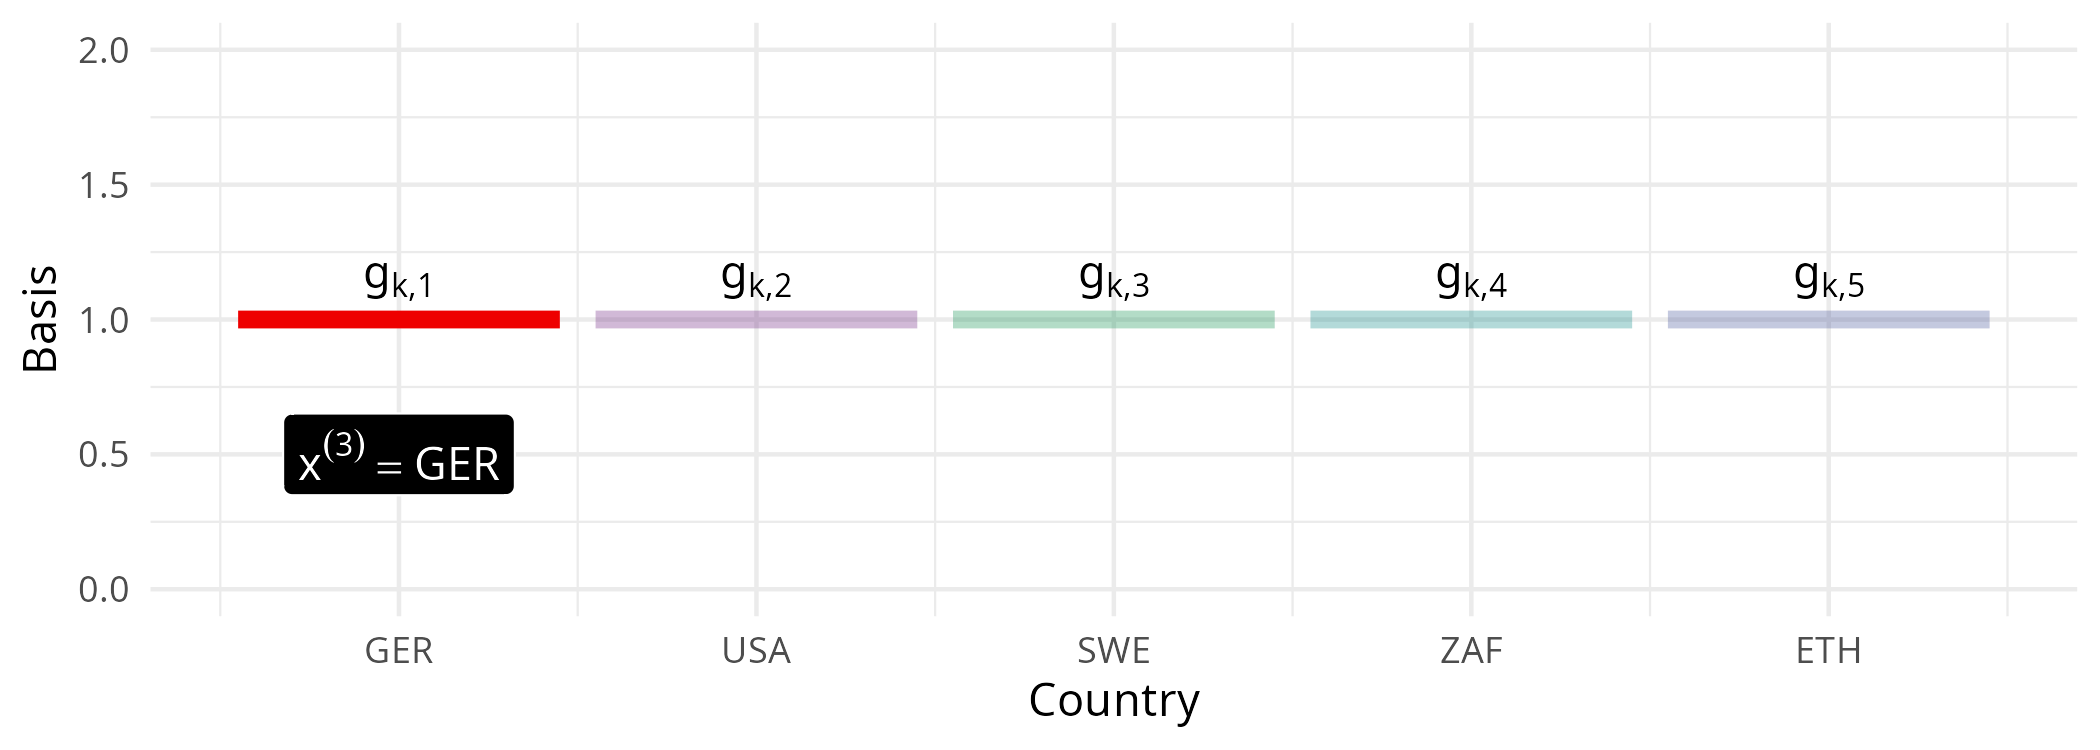
\includegraphics[width=0.7\textwidth]{figures/bs-cat/fig-cat3.png}
    \end{figure}
    \vspace{-0.5cm}
    \scriptsize
    $$
      \design_k = \begin{blockarray}{ccccc}
        \color[HTML]{EE0000}g_{k,GER} & \color[HTML]{631879}g_{k,USA} & \color[HTML]{008B45}g_{k,SWE} & \color[HTML]{008280}g_{k,ZAF} & \color[HTML]{3B4992}g_{k,ETH}\\
      \begin{block}{(ccccc)}
        \color{lightgray}0 & \color{black}\bm{1} & \color{lightgray}0 & \color{lightgray}0 & \color{lightgray}0 \\
      \color{lightgray}0 & \color{lightgray}0 & \color{lightgray}0 & \color{lightgray}0 & \color{black}\bm{1} \\
      \color[HTML]{EE0000}\bm{1} & \color{lightgray}0 & \color{lightgray}0 & \color{lightgray}0 & \color{lightgray}0 \\
      \color{white}\vdots & \color{white}\vdots & \color{white}\vdots & \color{white}\vdots & \color{white}\vdots \\
      \color{white}0 & \color{white}0 & \color{white}0 & \color{white}0 & \color{white}0 \\
      \color{white}0 & \color{white}0 & \color{white}0 & \color{white}0 & \color{white}0 \\
      \color{white}0 & \color{white}0 & \color{white}0 & \color{white}0 & \color{white}0 \color{black}\\
      \end{block}
    \end{blockarray}
    $$
    \normalsize
  \end{center}
\end{frame}

\begin{frame}{Component-wise gradient boosting -- Base learner examples II}
  \textbf{Categorical base learner} $g_k(x) = (g_{k,1}(x), \dots, g_{k,G}(x))^\tran = (\mathds{1}_{\{x = 1\}}, \dots, \mathds{1}_{\{x = G\}})^\tran$ with categorical $x\in\{1, \dots, G\}$.

  \begin{center}
    \begin{figure}
      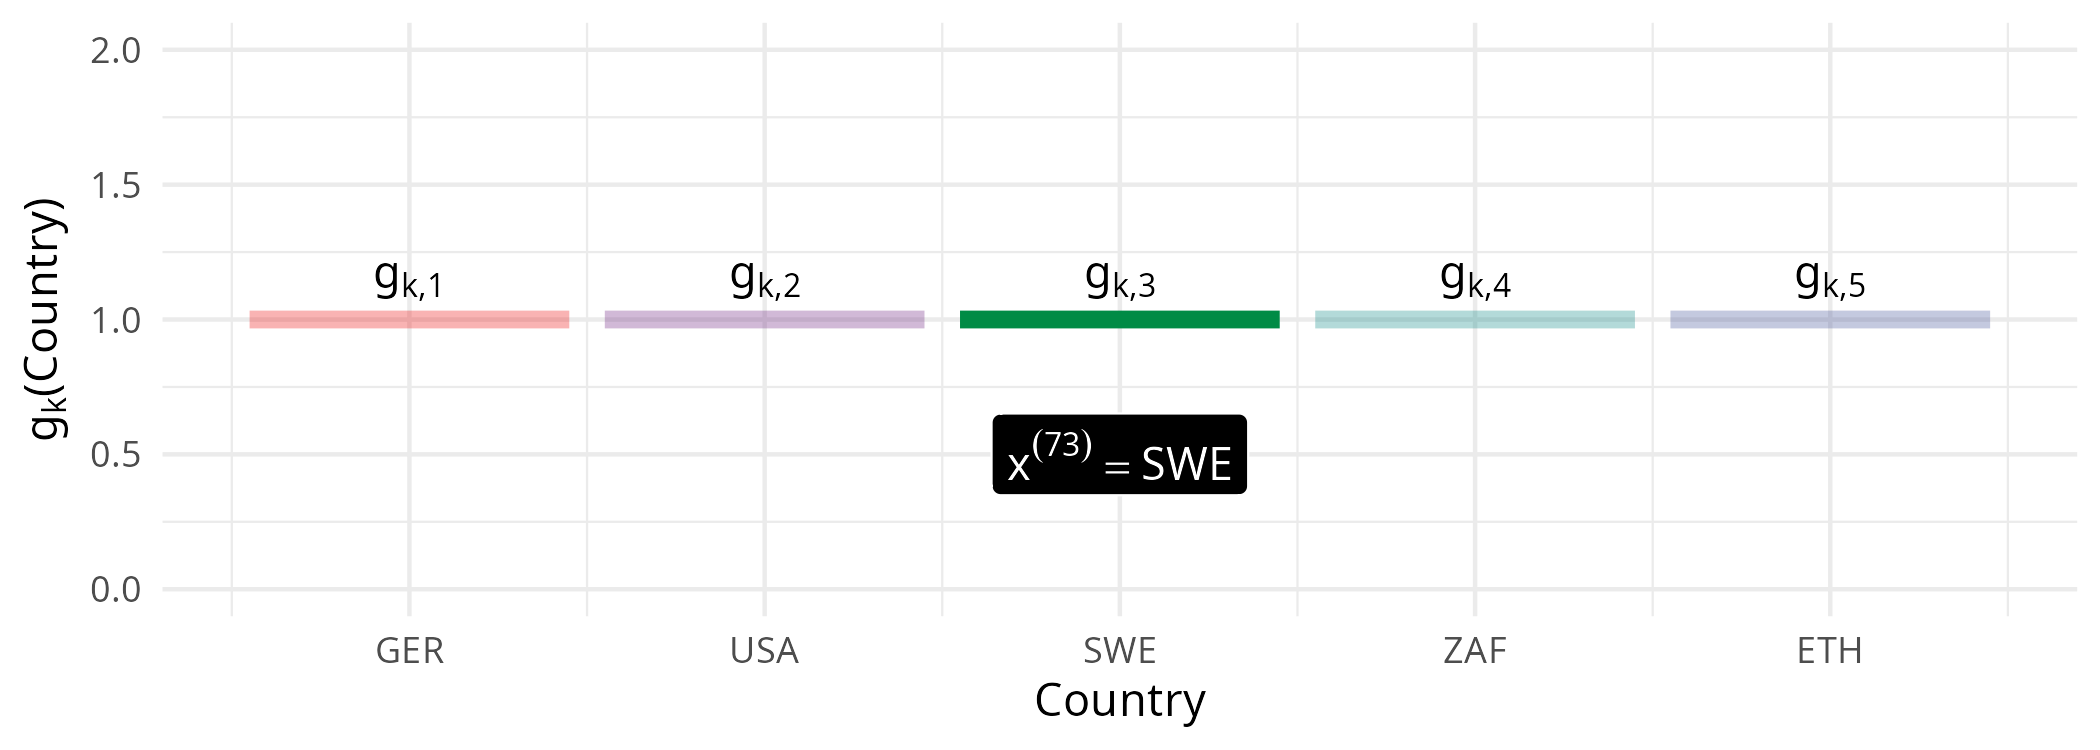
\includegraphics[width=0.7\textwidth]{figures/bs-cat/fig-cat4.png}
    \end{figure}
    \vspace{-0.5cm}
    \scriptsize
    $$
      \design_k = \begin{blockarray}{ccccc}
        \color[HTML]{EE0000}g_{k,GER} & \color[HTML]{631879}g_{k,USA} & \color[HTML]{008B45}g_{k,SWE} & \color[HTML]{008280}g_{k,ZAF} & \color[HTML]{3B4992}g_{k,ETH}\\
      \begin{block}{(ccccc)}
        \color{lightgray}0 & \color{black}\bm{1} & \color{lightgray}0 & \color{lightgray}0 & \color{lightgray}0 \\
      \color{lightgray}0 & \color{lightgray}0 & \color{lightgray}0 & \color{lightgray}0 & \color{black}\bm{1} \\
      \color{black}\bm{1} & \color{lightgray}0 & \color{lightgray}0 & \color{lightgray}0 & \color{lightgray}0 \\
      \color{lightgray}\vdots & \color{lightgray}\vdots & \color{lightgray}\vdots & \color{lightgray}\vdots & \color{lightgray}\vdots \\
      \color{lightgray}0 & \color{lightgray}0 & \color[HTML]{008B45}\bm{1} & \color{lightgray}0 & \color{lightgray}0 \\
      \color{white}0 & \color{white}0 & \color{white}0 & \color{white}0 & \color{white}0 \\
      \color{white}0 & \color{white}0 & \color{white}0 & \color{white}0 & \color{white}0 \color{black}\\
      \end{block}
    \end{blockarray}
    $$
    \normalsize
  \end{center}
\end{frame}

\begin{frame}{Component-wise gradient boosting -- Base learner examples II}
  \textbf{Categorical base learner} $g_k(x) = (g_{k,1}(x), \dots, g_{k,G}(x))^\tran = (\mathds{1}_{\{x = 1\}}, \dots, \mathds{1}_{\{x = G\}})^\tran$ with categorical $x\in\{1, \dots, G\}$.

  \begin{center}
    \begin{figure}
      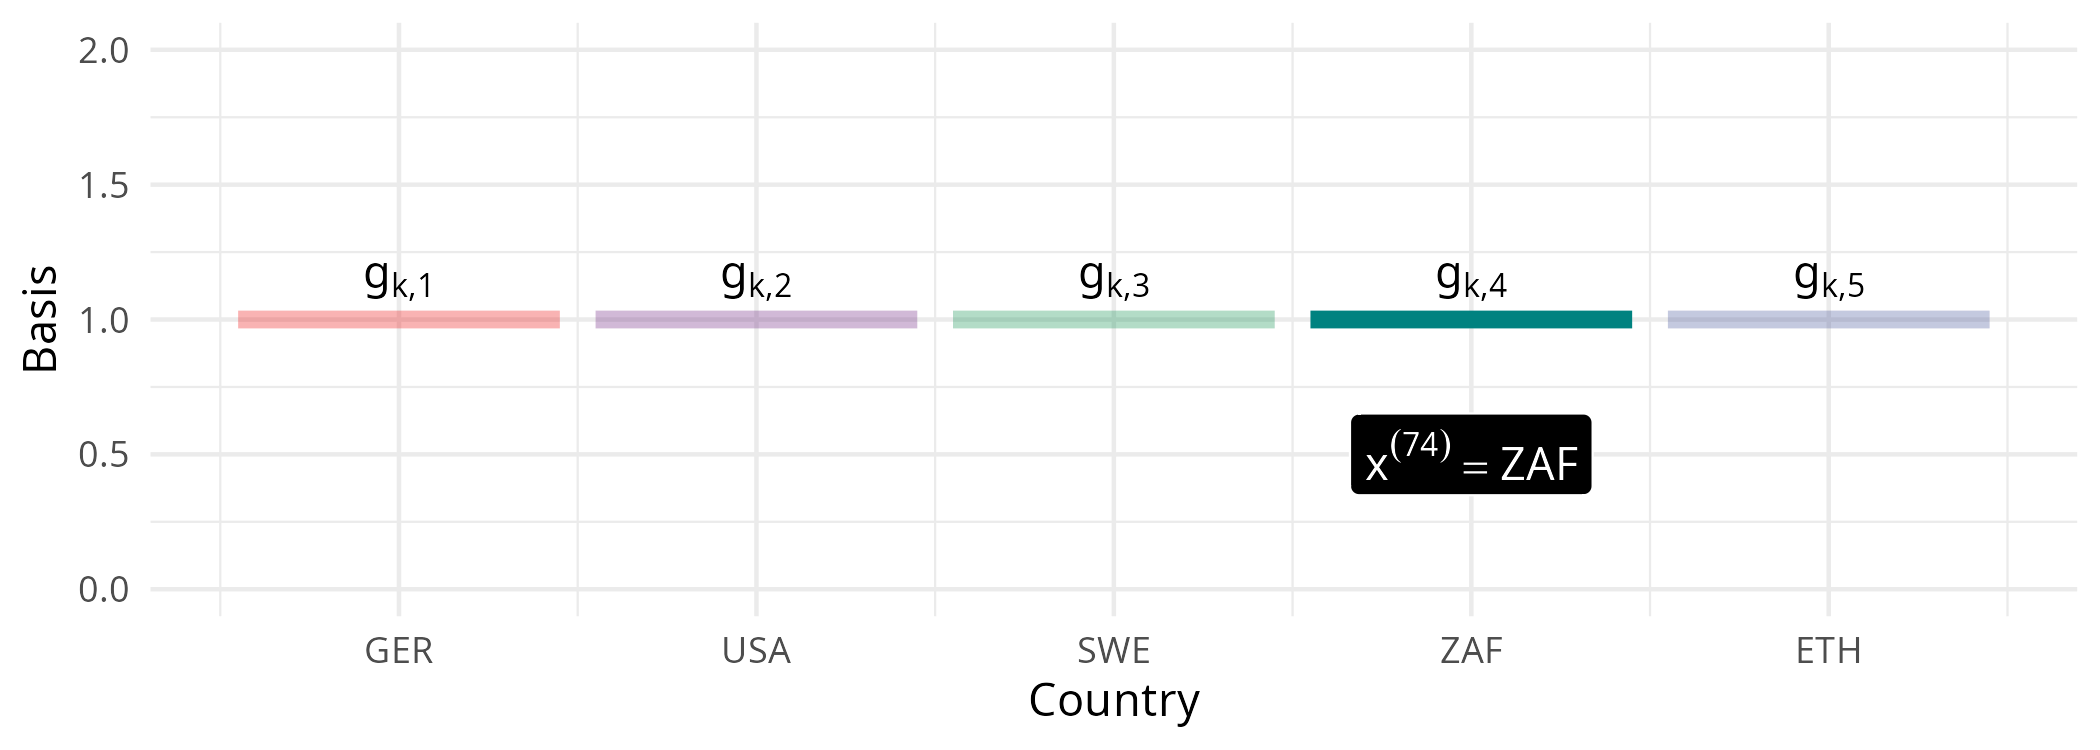
\includegraphics[width=0.7\textwidth]{figures/bs-cat/fig-cat5.png}
    \end{figure}
    \vspace{-0.5cm}
    \scriptsize
    $$
      \design_k = \begin{blockarray}{ccccc}
        \color[HTML]{EE0000}g_{k,GER} & \color[HTML]{631879}g_{k,USA} & \color[HTML]{008B45}g_{k,SWE} & \color[HTML]{008280}g_{k,ZAF} & \color[HTML]{3B4992}g_{k,ETH}\\
      \begin{block}{(ccccc)}
        \color{lightgray}0 & \color{black}\bm{1} & \color{lightgray}0 & \color{lightgray}0 & \color{lightgray}0 \\
      \color{lightgray}0 & \color{lightgray}0 & \color{lightgray}0 & \color{lightgray}0 & \color{black}\bm{1} \\
      \color{black}\bm{1} & \color{lightgray}0 & \color{lightgray}0 & \color{lightgray}0 & \color{lightgray}0 \\
      \color{lightgray}\vdots & \color{lightgray}\vdots & \color{lightgray}\vdots & \color{lightgray}\vdots & \color{lightgray}\vdots \\
      \color{lightgray}0 & \color{lightgray}0 & \color{black}\bm{1} & \color{lightgray}0 & \color{lightgray}0 \\
      \color{lightgray}0 & \color{lightgray}0 & \color{lightgray}0 & \color[HTML]{008280}\bm{1} & \color{lightgray}0 \\
      \color{white}0 & \color{white}0 & \color{white}0 & \color{white}0 & \color{white}0 \color{black}\\
      \end{block}
    \end{blockarray}
    $$
    \normalsize
  \end{center}
\end{frame}

\begin{frame}{Component-wise gradient boosting -- Base learner examples II}
  \textbf{Categorical base learner} $g_k(x) = (g_{k,1}(x), \dots, g_{k,G}(x))^\tran = (\mathds{1}_{\{x = 1\}}, \dots, \mathds{1}_{\{x = G\}})^\tran$ with categorical $x\in\{1, \dots, G\}$.

  \begin{center}
    \begin{figure}
      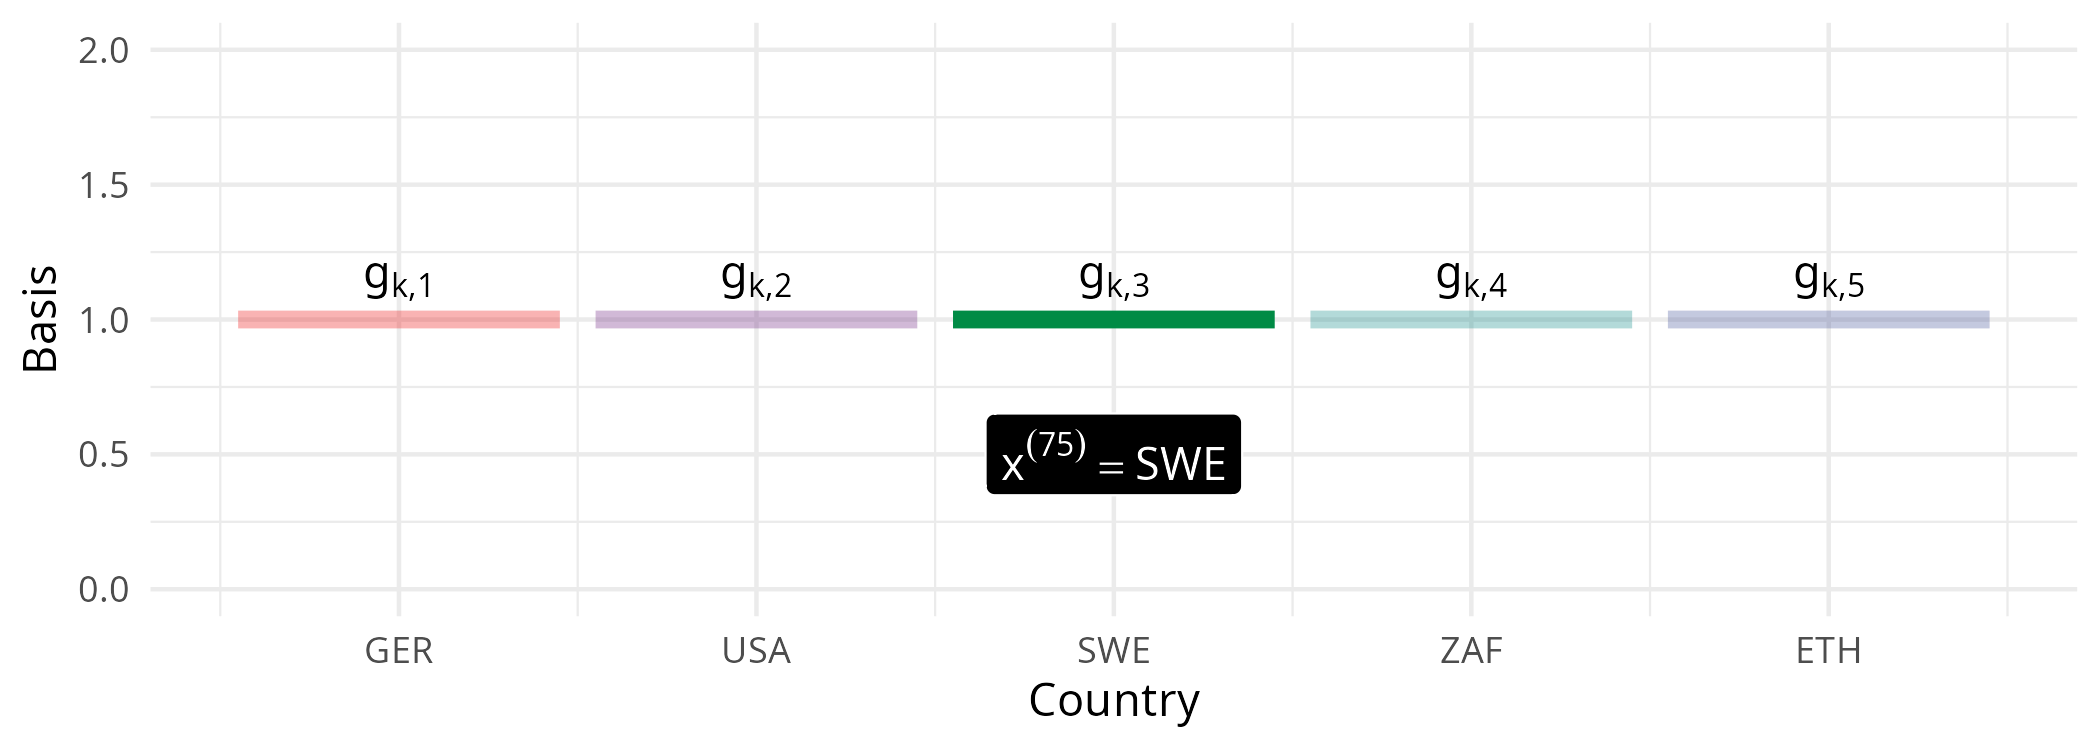
\includegraphics[width=0.7\textwidth]{figures/bs-cat/fig-cat6.png}
    \end{figure}
    \vspace{-0.5cm}
    \scriptsize
    $$
      \design_k = \begin{blockarray}{ccccc}
        \color[HTML]{EE0000}g_{k,GER} & \color[HTML]{631879}g_{k,USA} & \color[HTML]{008B45}g_{k,SWE} & \color[HTML]{008280}g_{k,ZAF} & \color[HTML]{3B4992}g_{k,ETH}\\
      \begin{block}{(ccccc)}
        \color{lightgray}0 & \color{black}\bm{1} & \color{lightgray}0 & \color{lightgray}0 & \color{lightgray}0 \\
      \color{lightgray}0 & \color{lightgray}0 & \color{lightgray}0 & \color{lightgray}0 & \color{black}\bm{1} \\
      \color{black}\bm{1} & \color{lightgray}0 & \color{lightgray}0 & \color{lightgray}0 & \color{lightgray}0 \\
      \color{lightgray}\vdots & \color{lightgray}\vdots & \color{lightgray}\vdots & \color{lightgray}\vdots & \color{lightgray}\vdots \\
      \color{lightgray}0 & \color{lightgray}0 & \color{008B45}\bm{1} & \color{lightgray}0 & \color{lightgray}0 \\
      \color{lightgray}0 & \color{lightgray}0 & \color{lightgray}0 & \color{black}\bm{1} & \color{lightgray}0 \\
      \color{lightgray}0 & \color{lightgray}0 & \color[HTML]{008B45}\bm{1} & \color{lightgray}0 & \color{lightgray}0 \\
      \end{block}
    \end{blockarray}
    $$
    \normalsize
  \end{center}
\end{frame}






\begin{frame}{Component-wise gradient boosting -- Base learner examples III}
  \textbf{Tensor product base learner}
\end{frame}

\begin{frame}{Initialization vs. fitting phase}
\end{frame}

%
\begin{frame}{Example: Life expectancy (nonlinear)}
	\begin{figure}
		\centering
		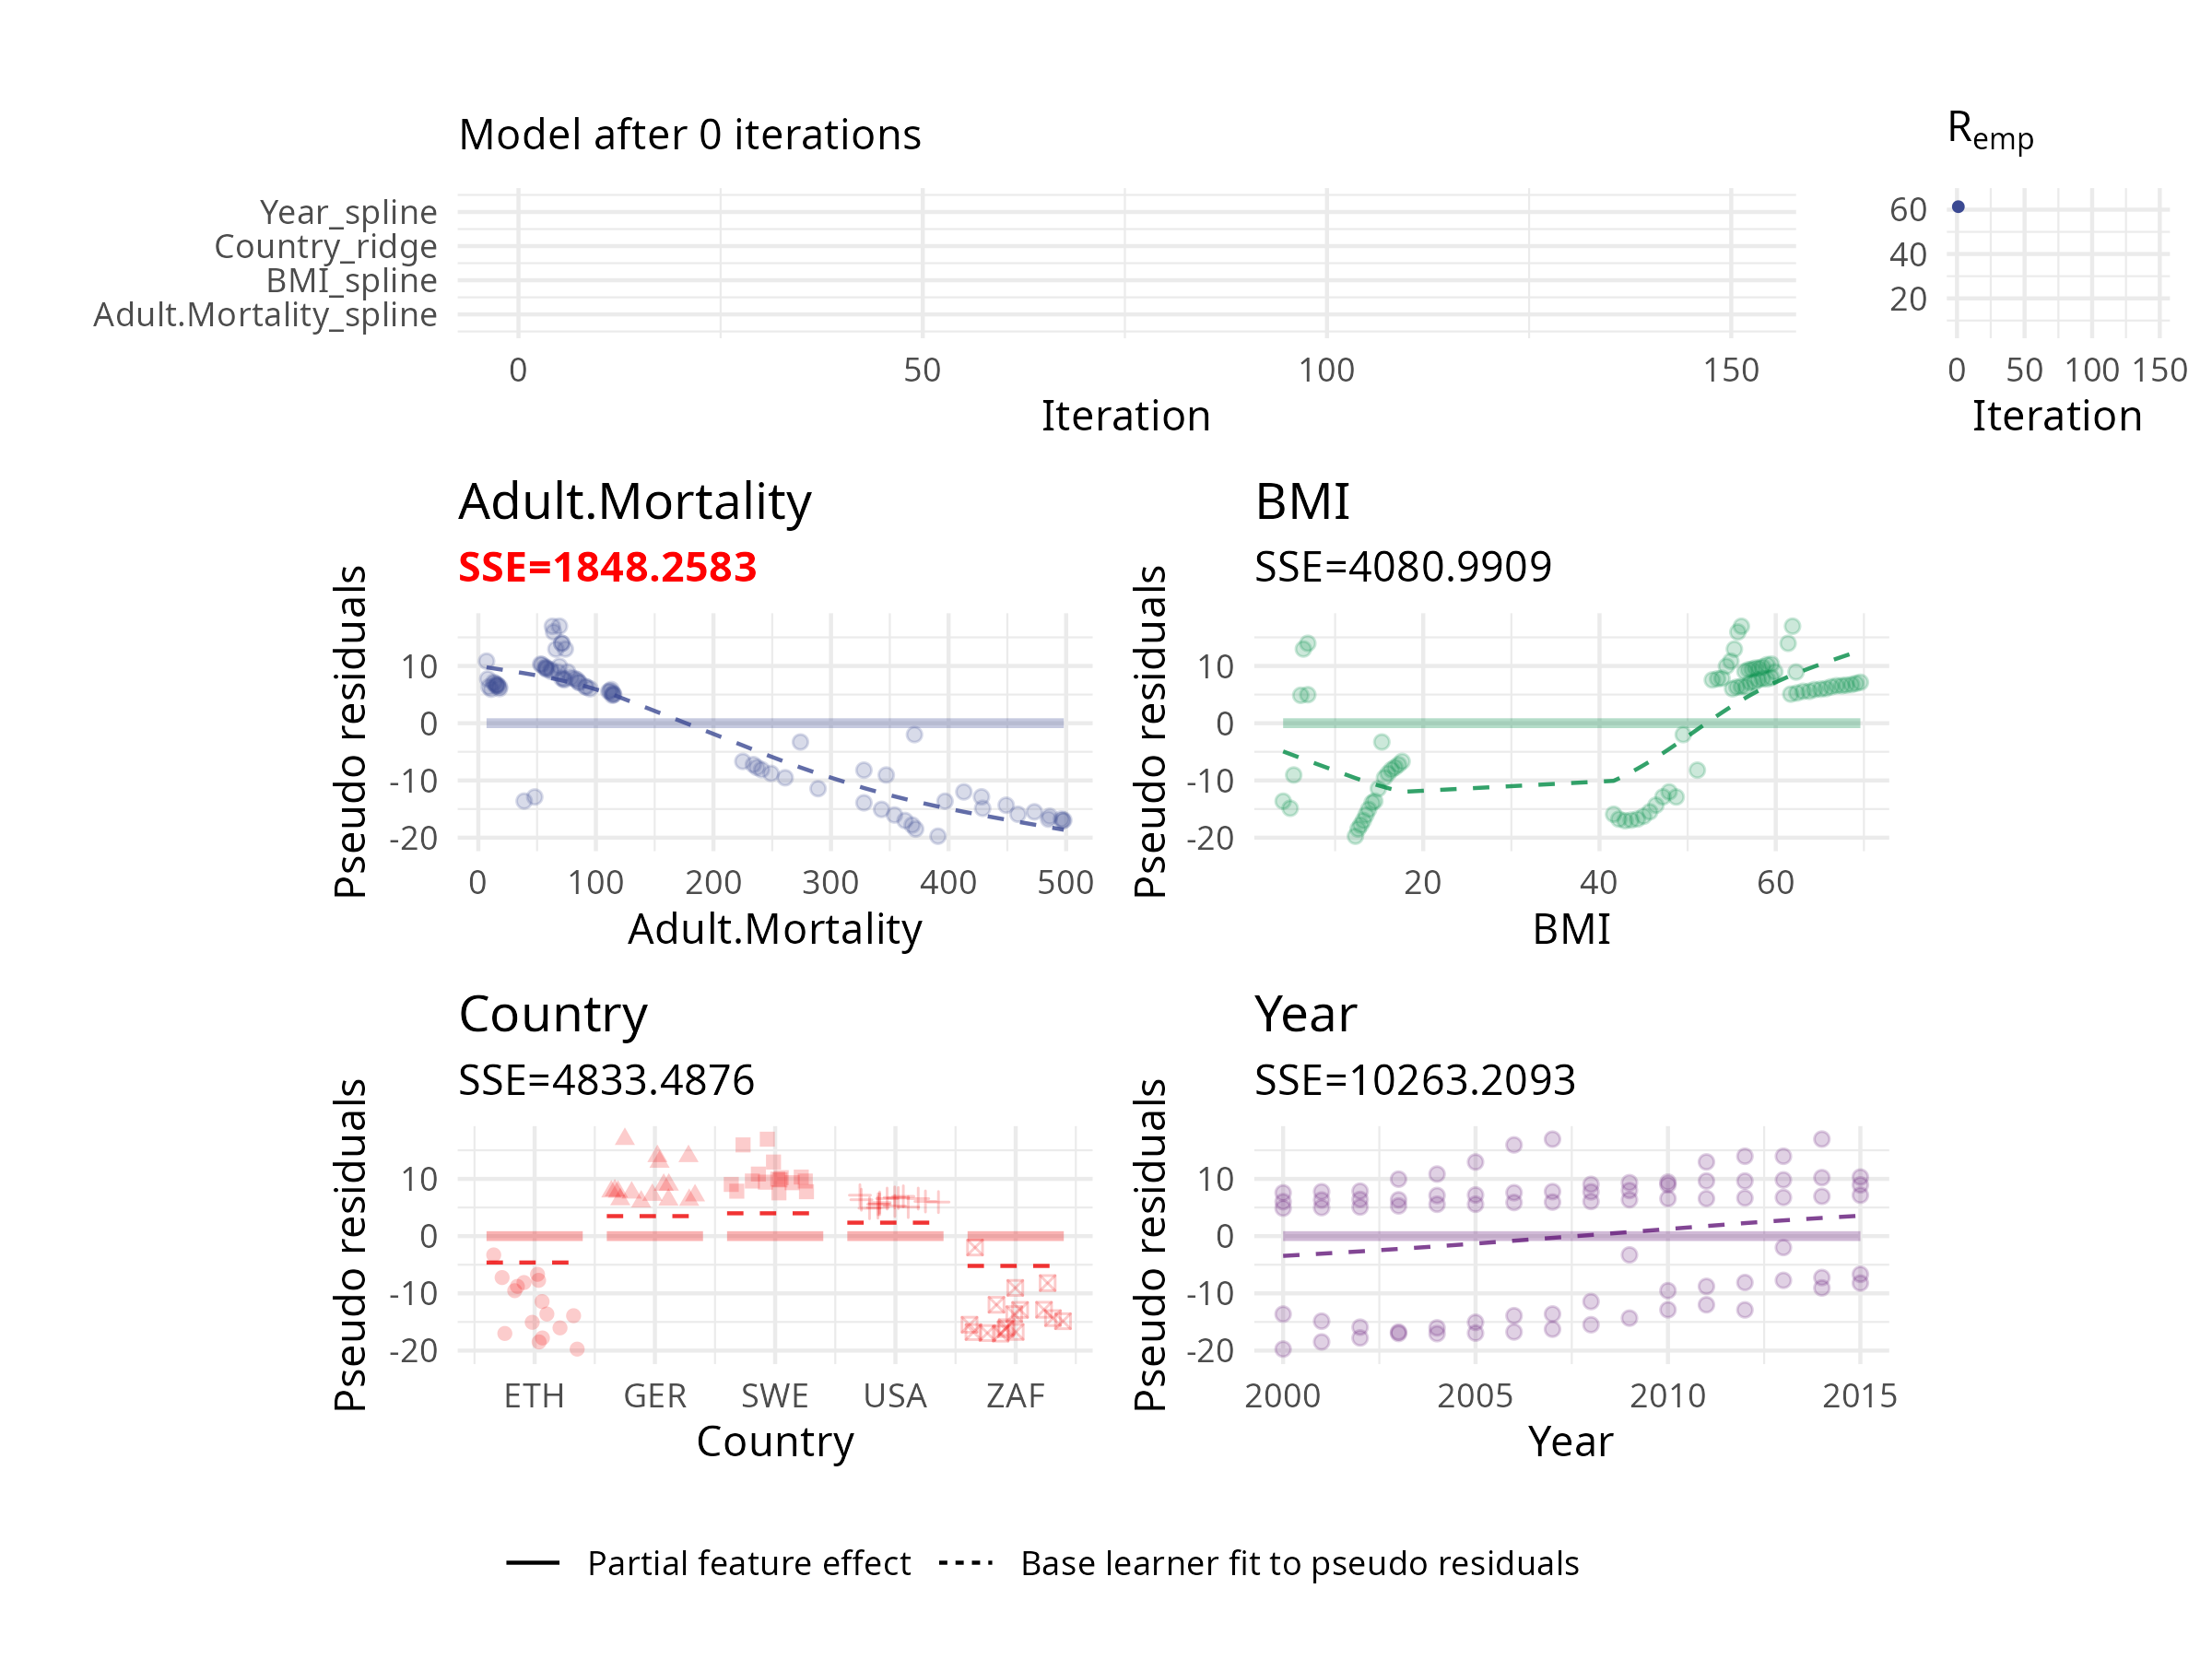
\includegraphics[width=\textwidth]{figures/cwb-anim/fig-iter-0001.png}
	\end{figure}
	\addtocounter{framenumber}{0}
\end{frame}


\begin{frame}{Example: Life expectancy (nonlinear)}
	\begin{figure}
		\centering
		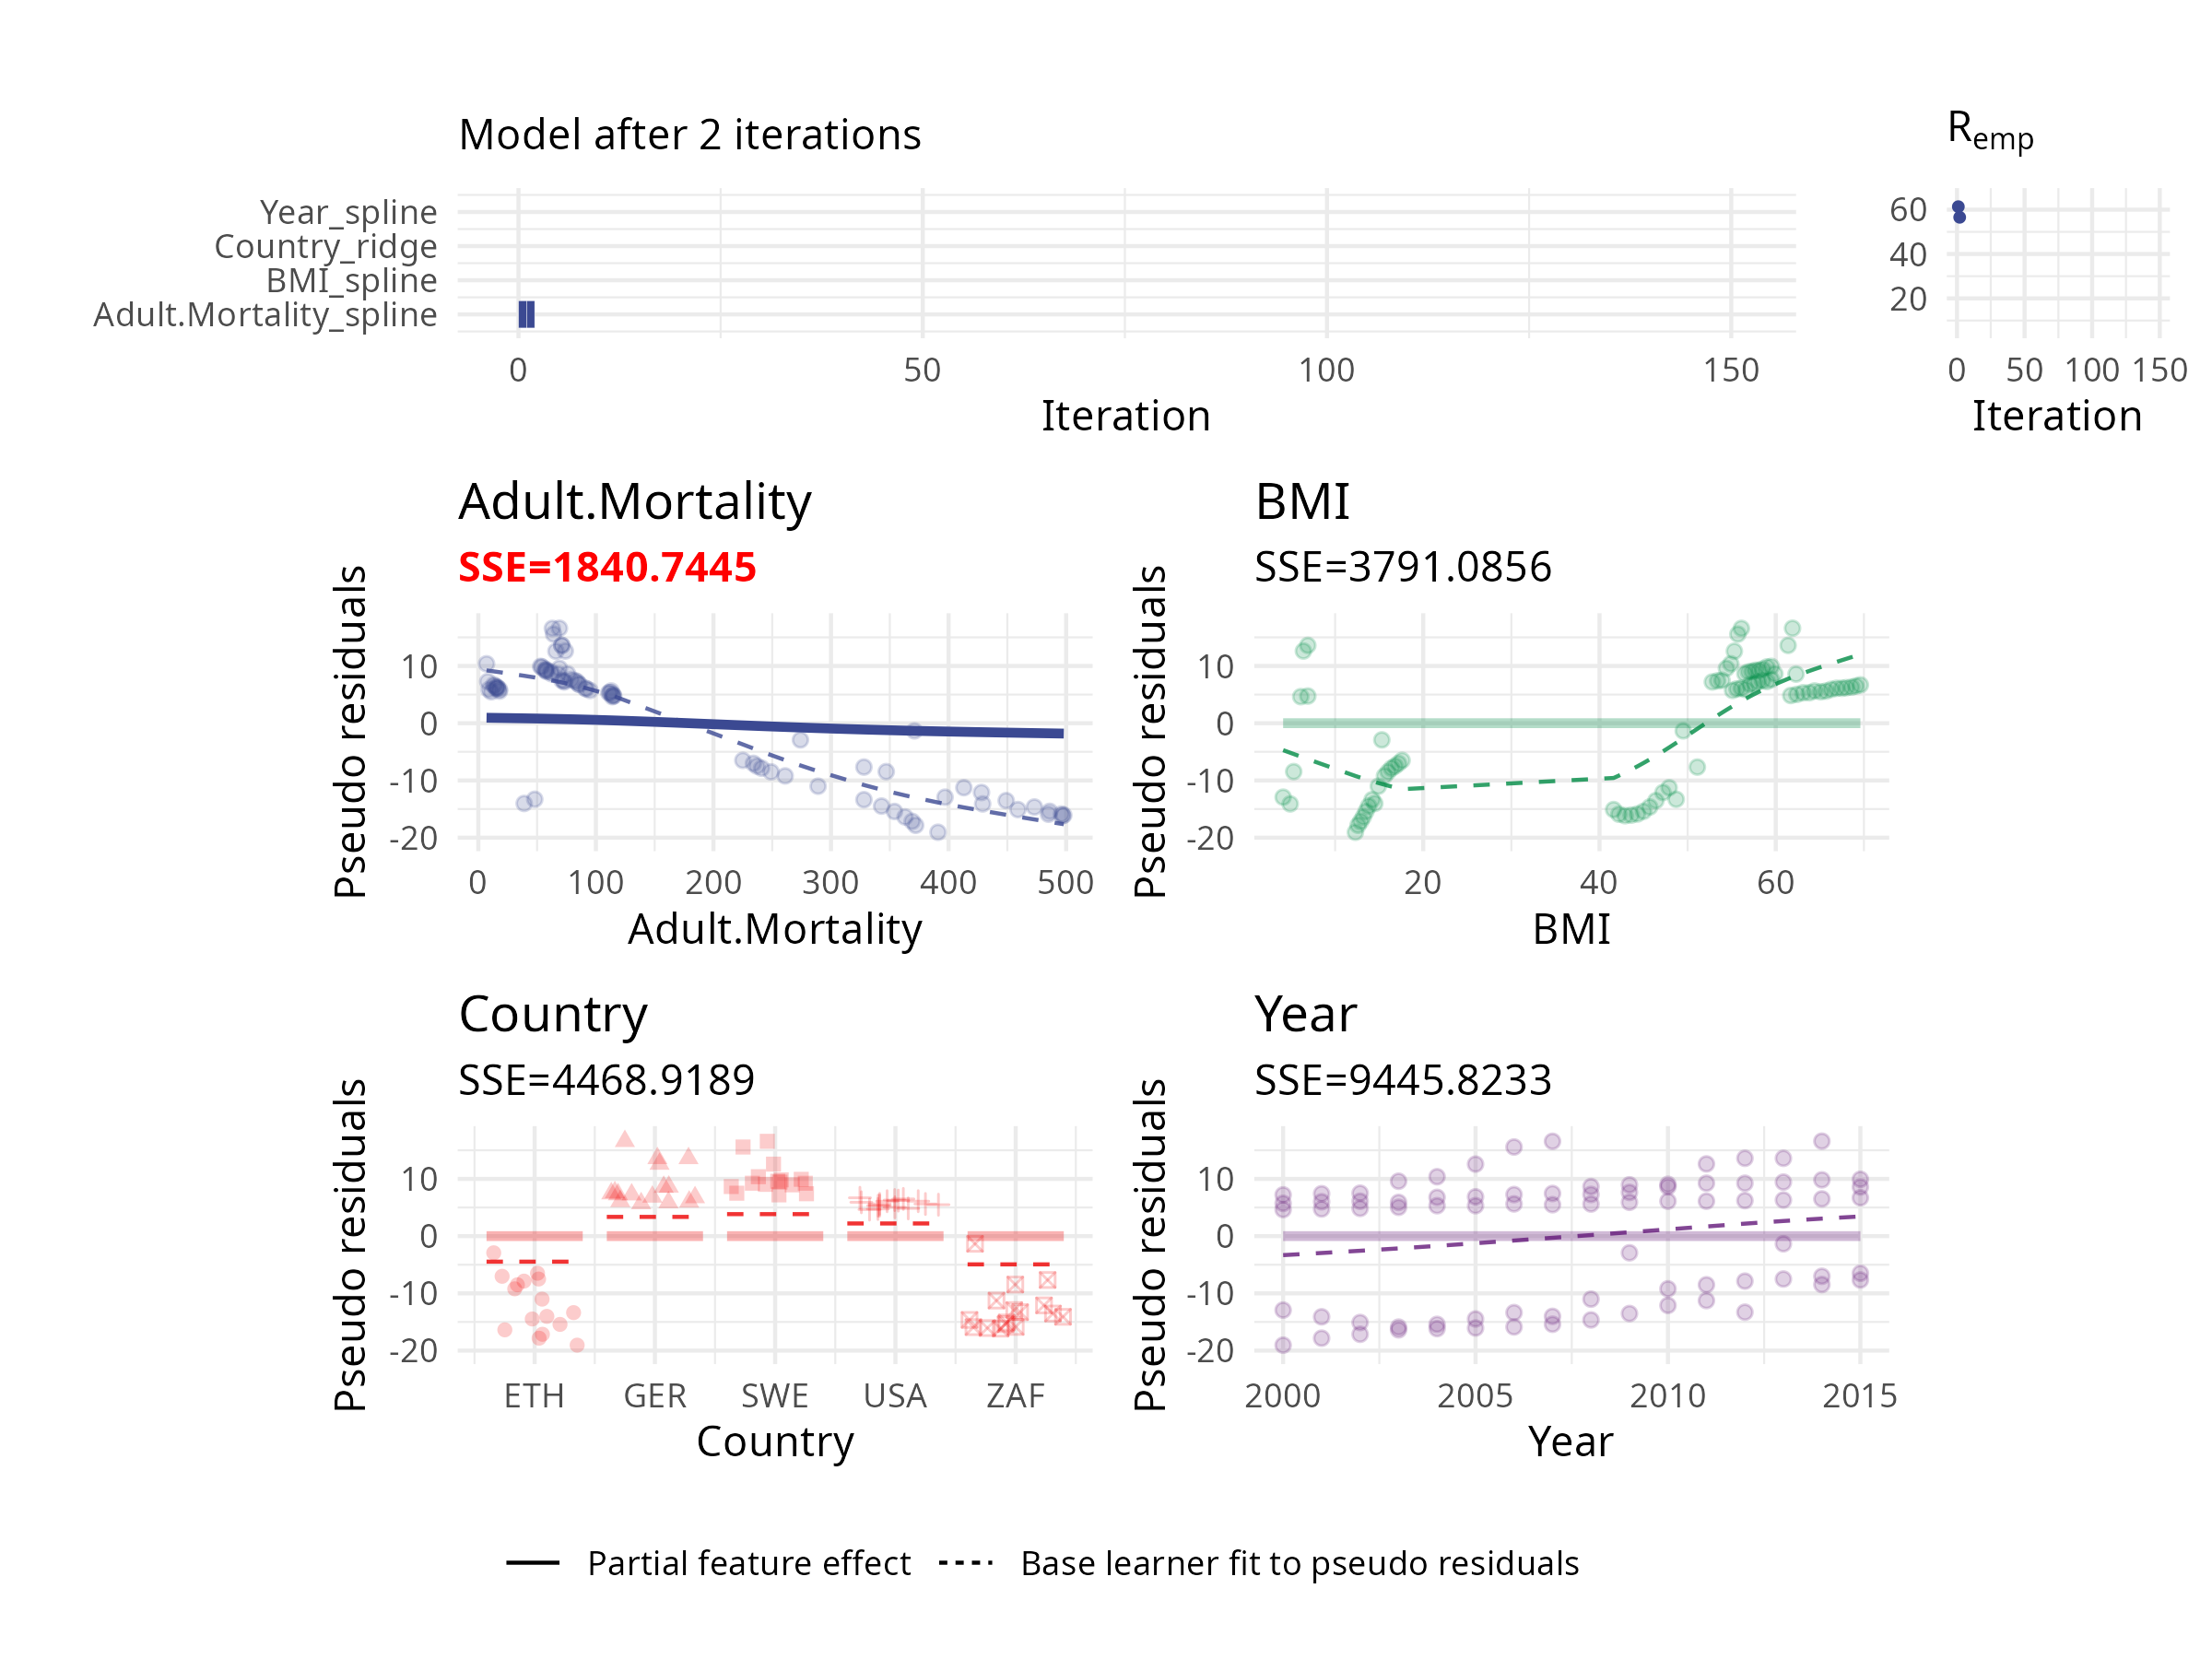
\includegraphics[width=\textwidth]{figures/cwb-anim/fig-iter-0002.png}
	\end{figure}
	\addtocounter{framenumber}{-1}
\end{frame}


\begin{frame}{Example: Life expectancy (nonlinear)}
	\begin{figure}
		\centering
		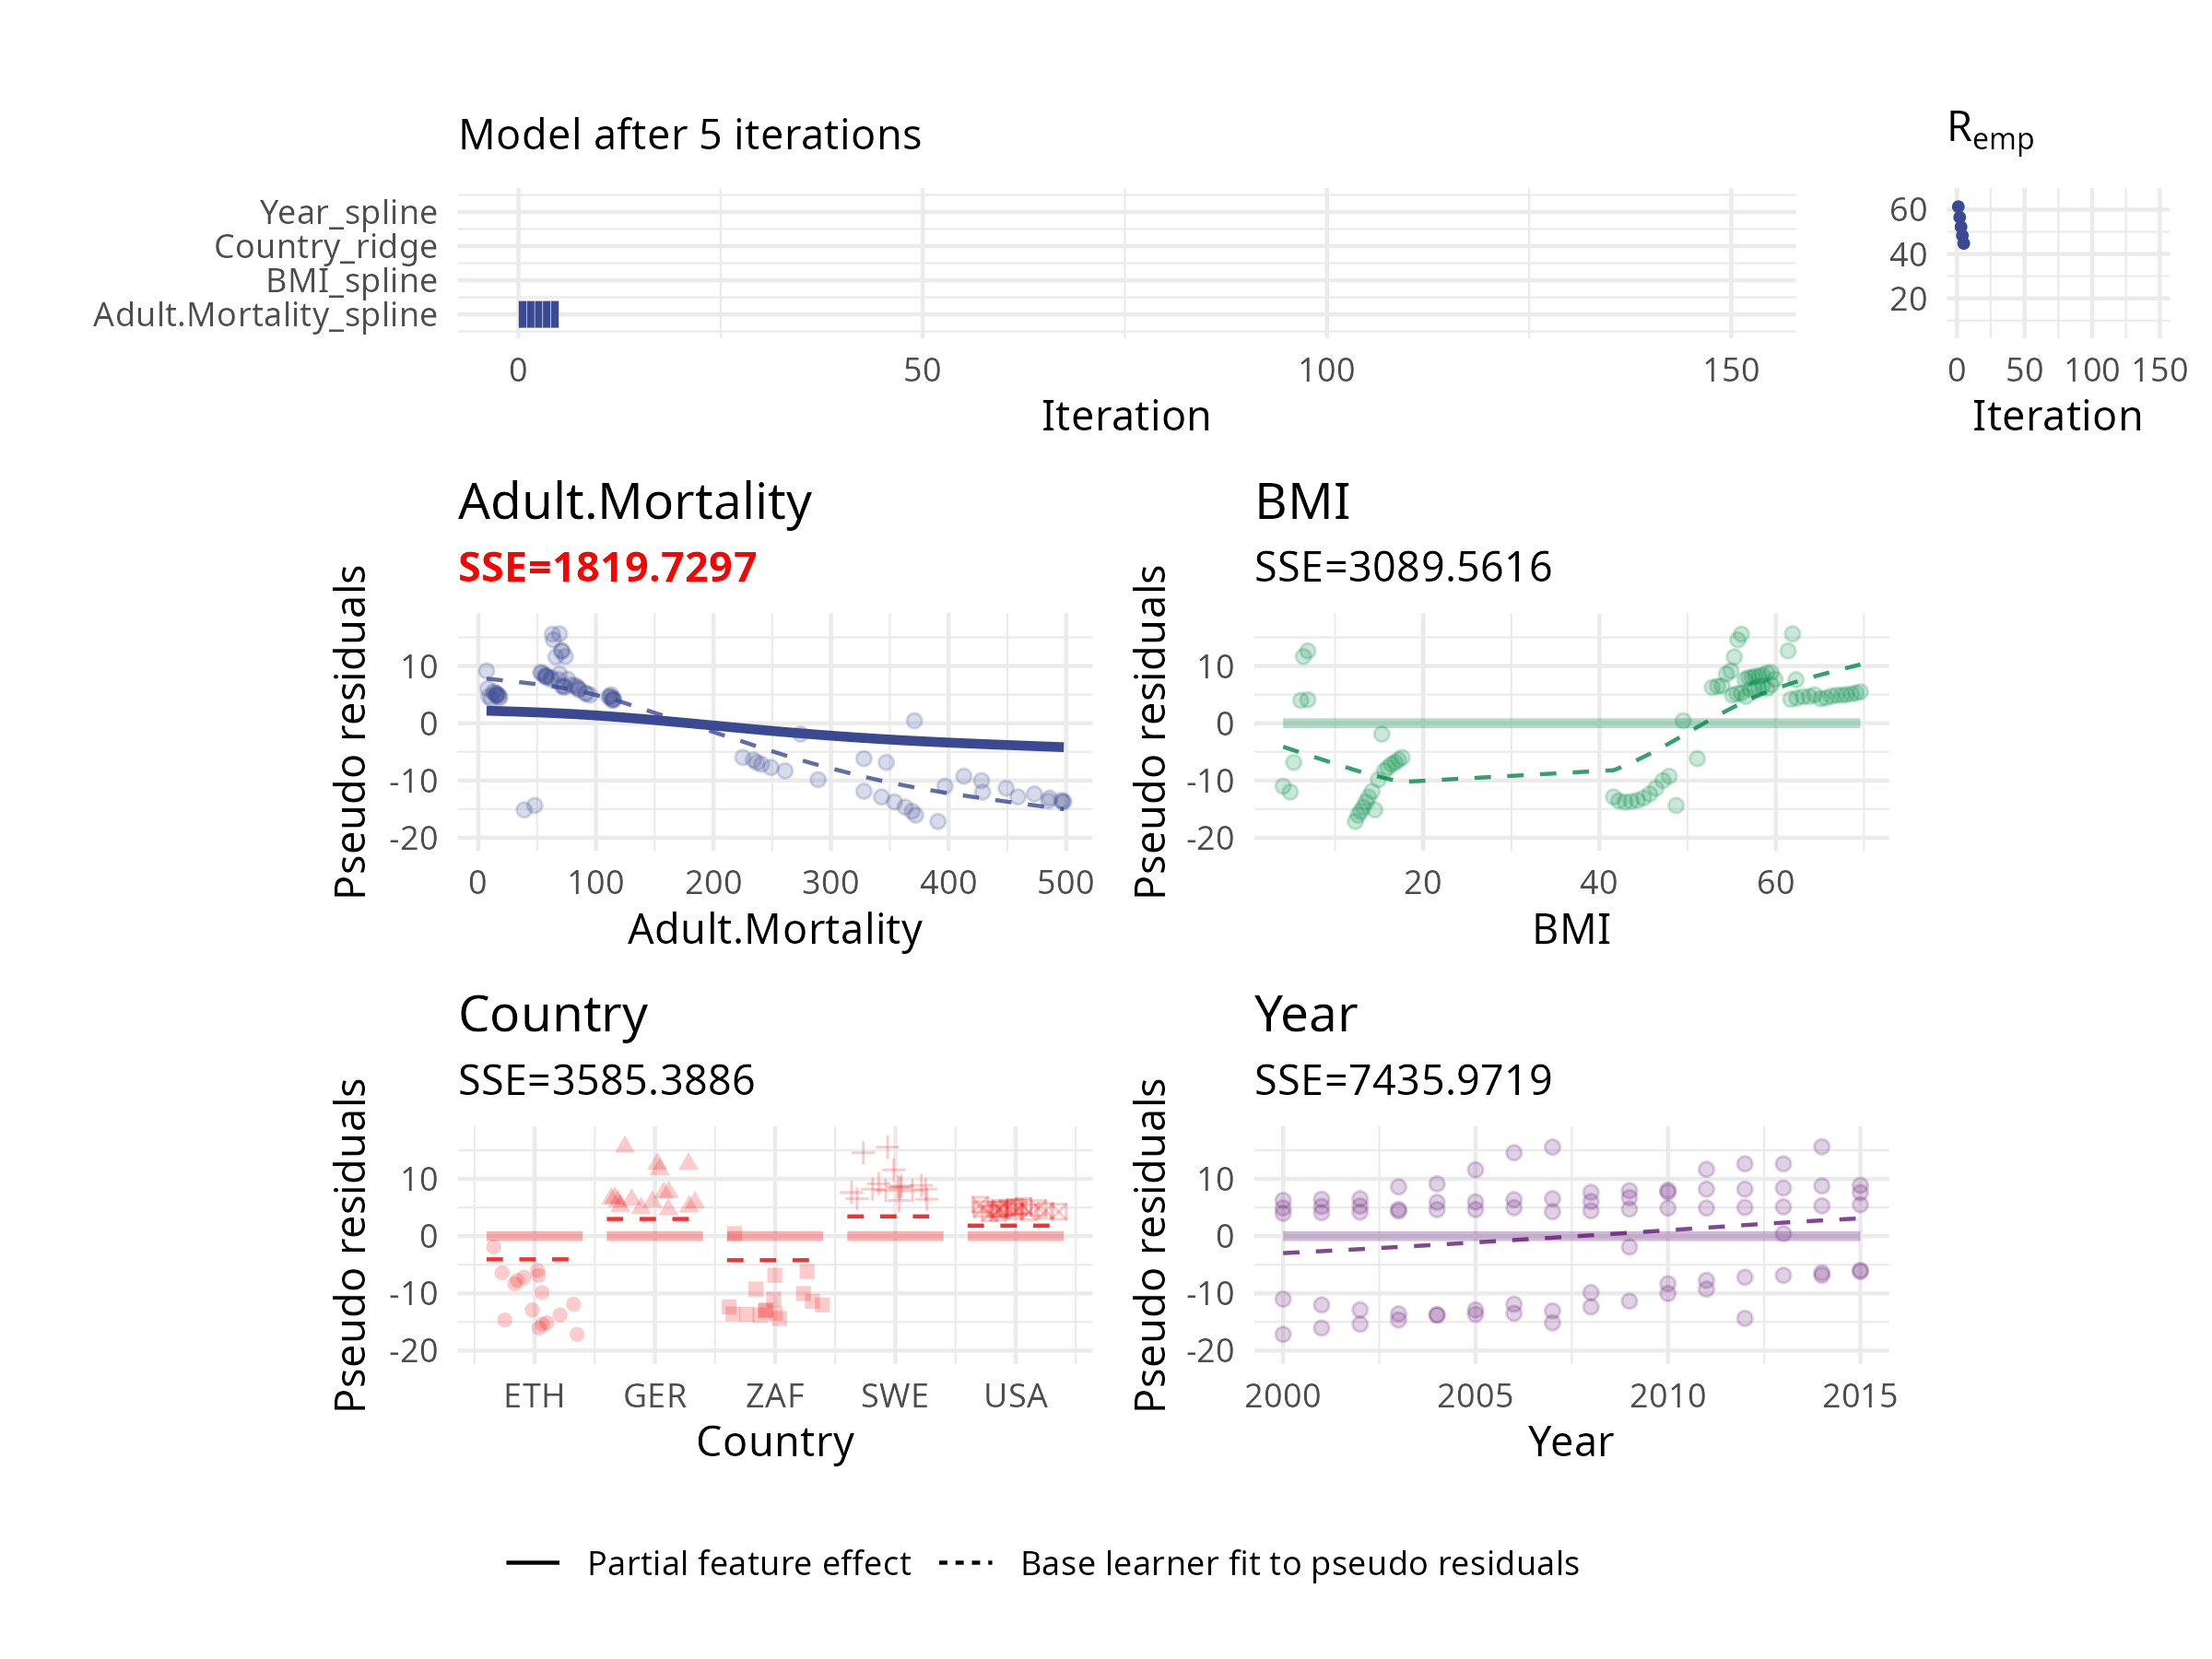
\includegraphics[width=\textwidth]{figures/cwb-anim/fig-iter-0005.png}
	\end{figure}
	\addtocounter{framenumber}{-1}
\end{frame}


\begin{frame}{Example: Life expectancy (nonlinear)}
	\begin{figure}
		\centering
		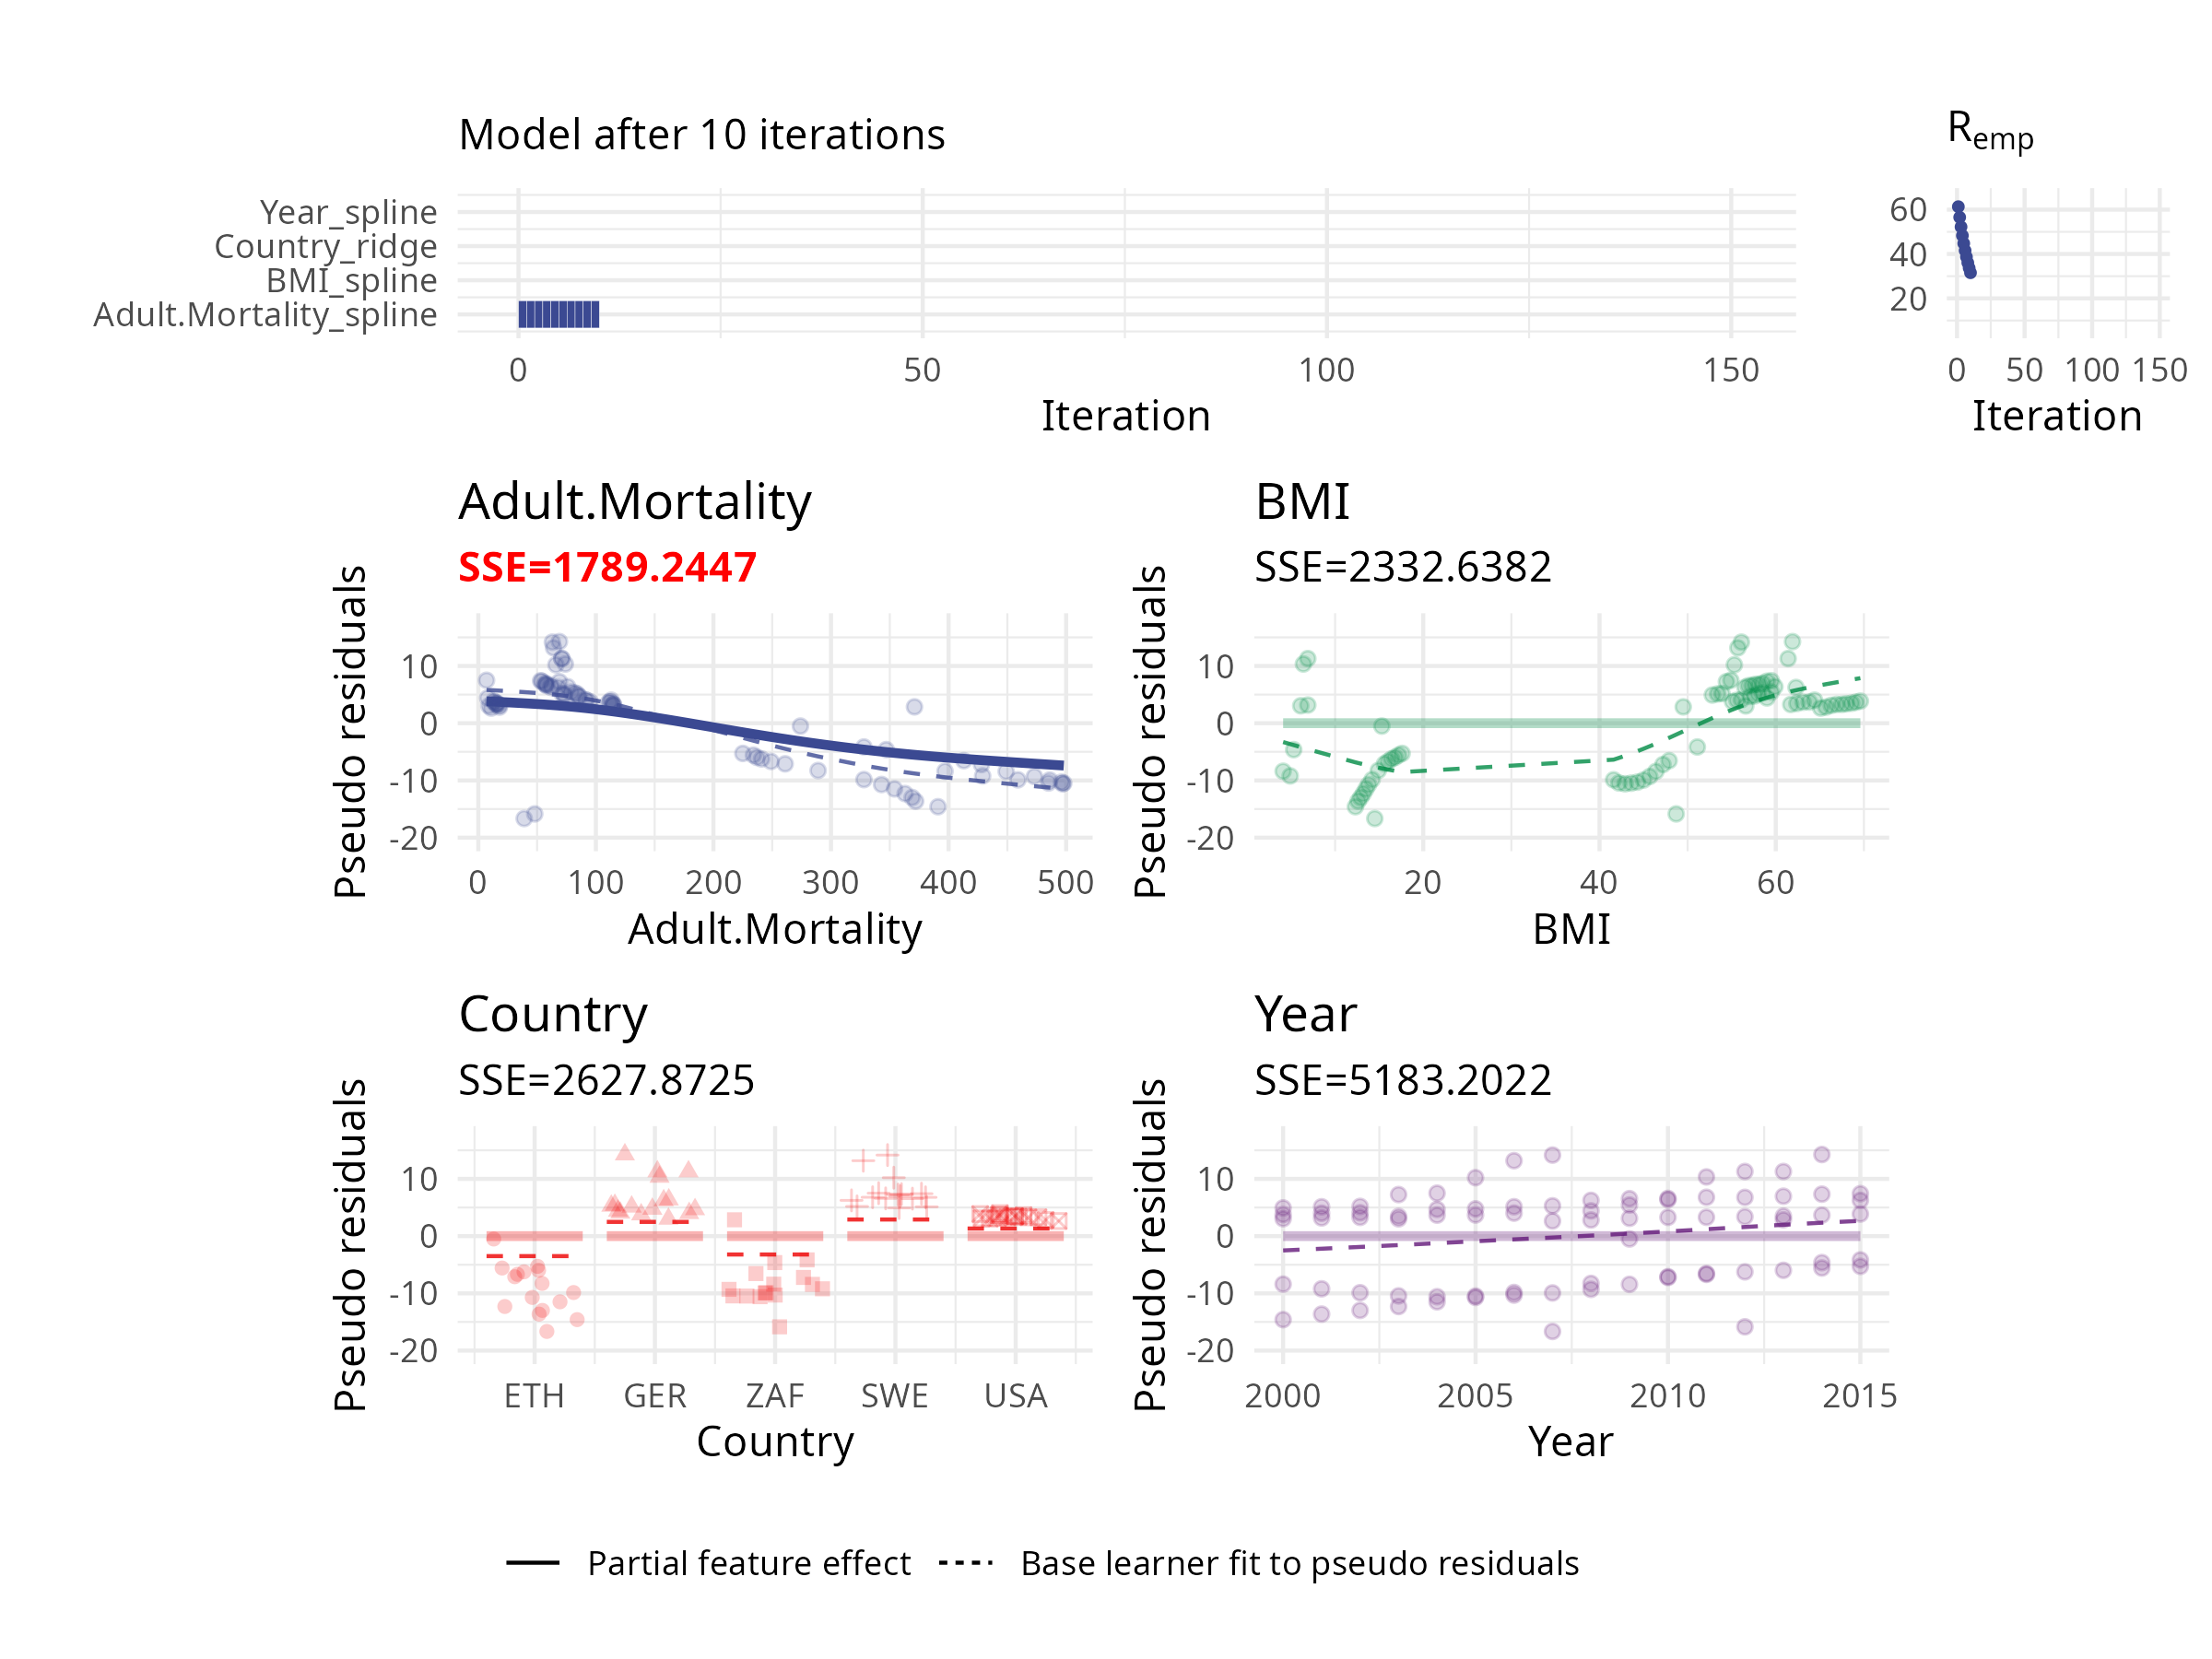
\includegraphics[width=\textwidth]{figures/cwb-anim/fig-iter-0010.png}
	\end{figure}
	\addtocounter{framenumber}{-1}
\end{frame}


\begin{frame}{Example: Life expectancy (nonlinear)}
	\begin{figure}
		\centering
		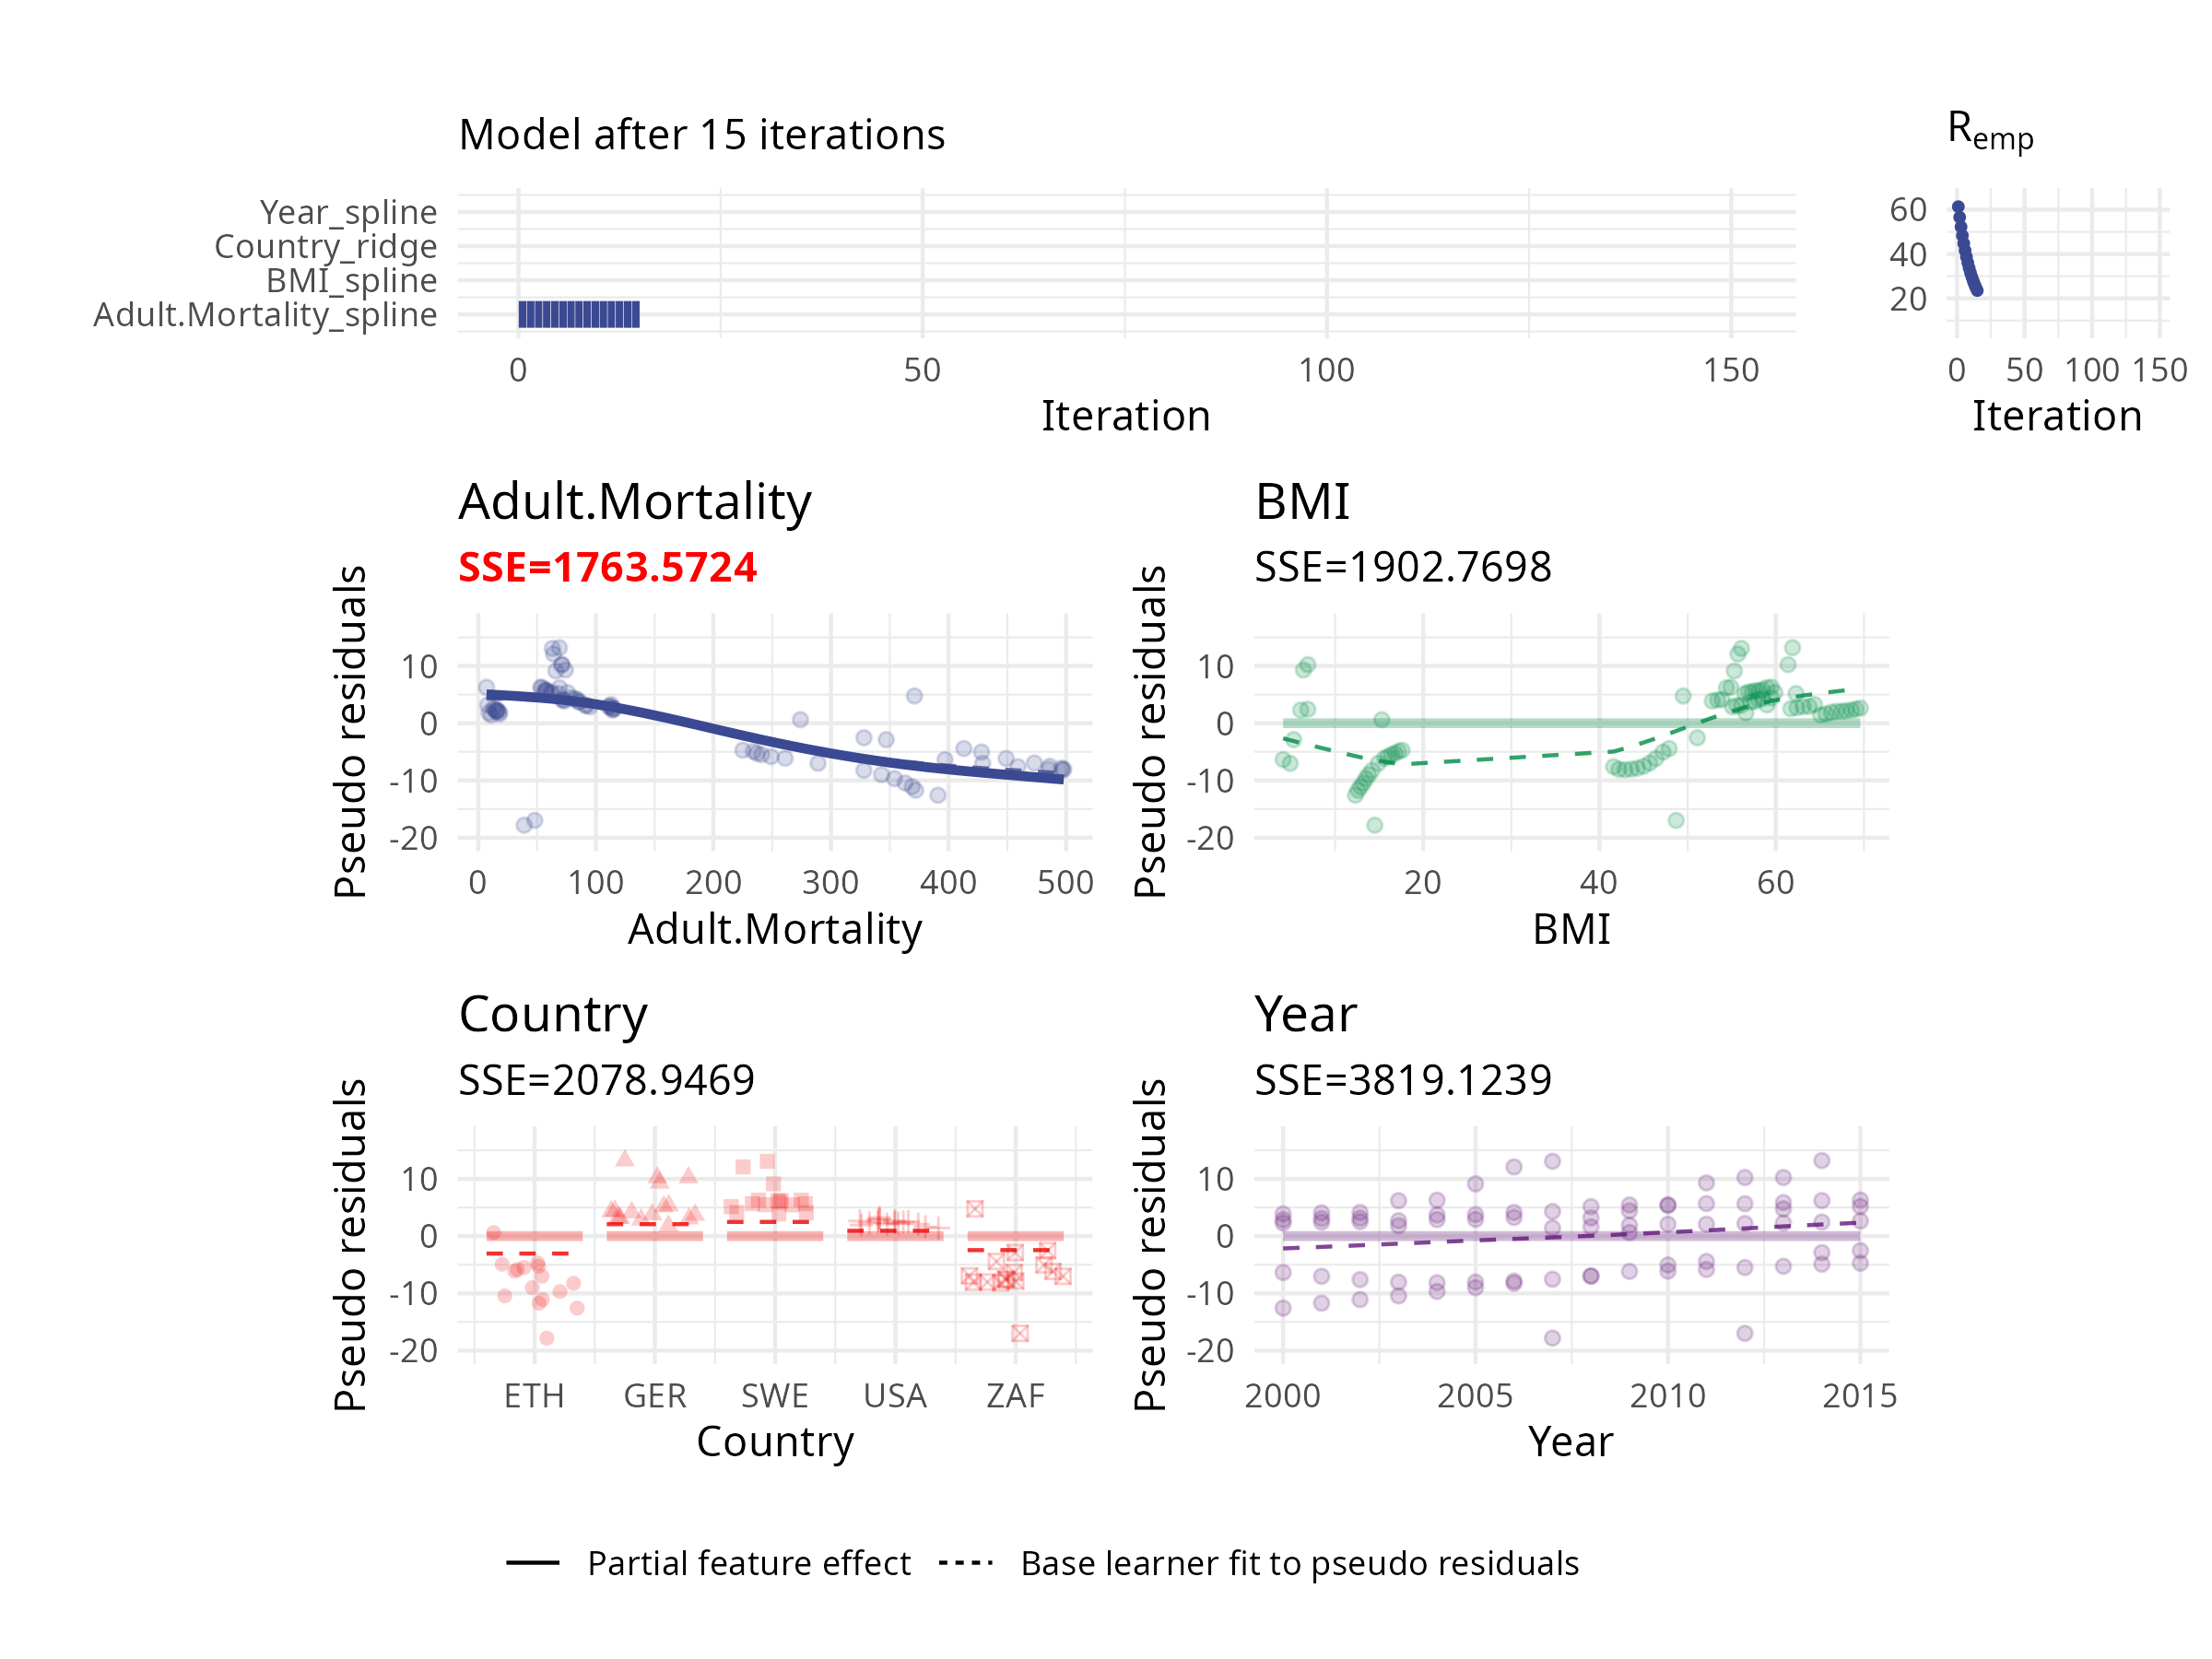
\includegraphics[width=\textwidth]{figures/cwb-anim/fig-iter-0015.png}
	\end{figure}
	\addtocounter{framenumber}{-1}
\end{frame}


\begin{frame}{Example: Life expectancy (nonlinear)}
	\begin{figure}
		\centering
		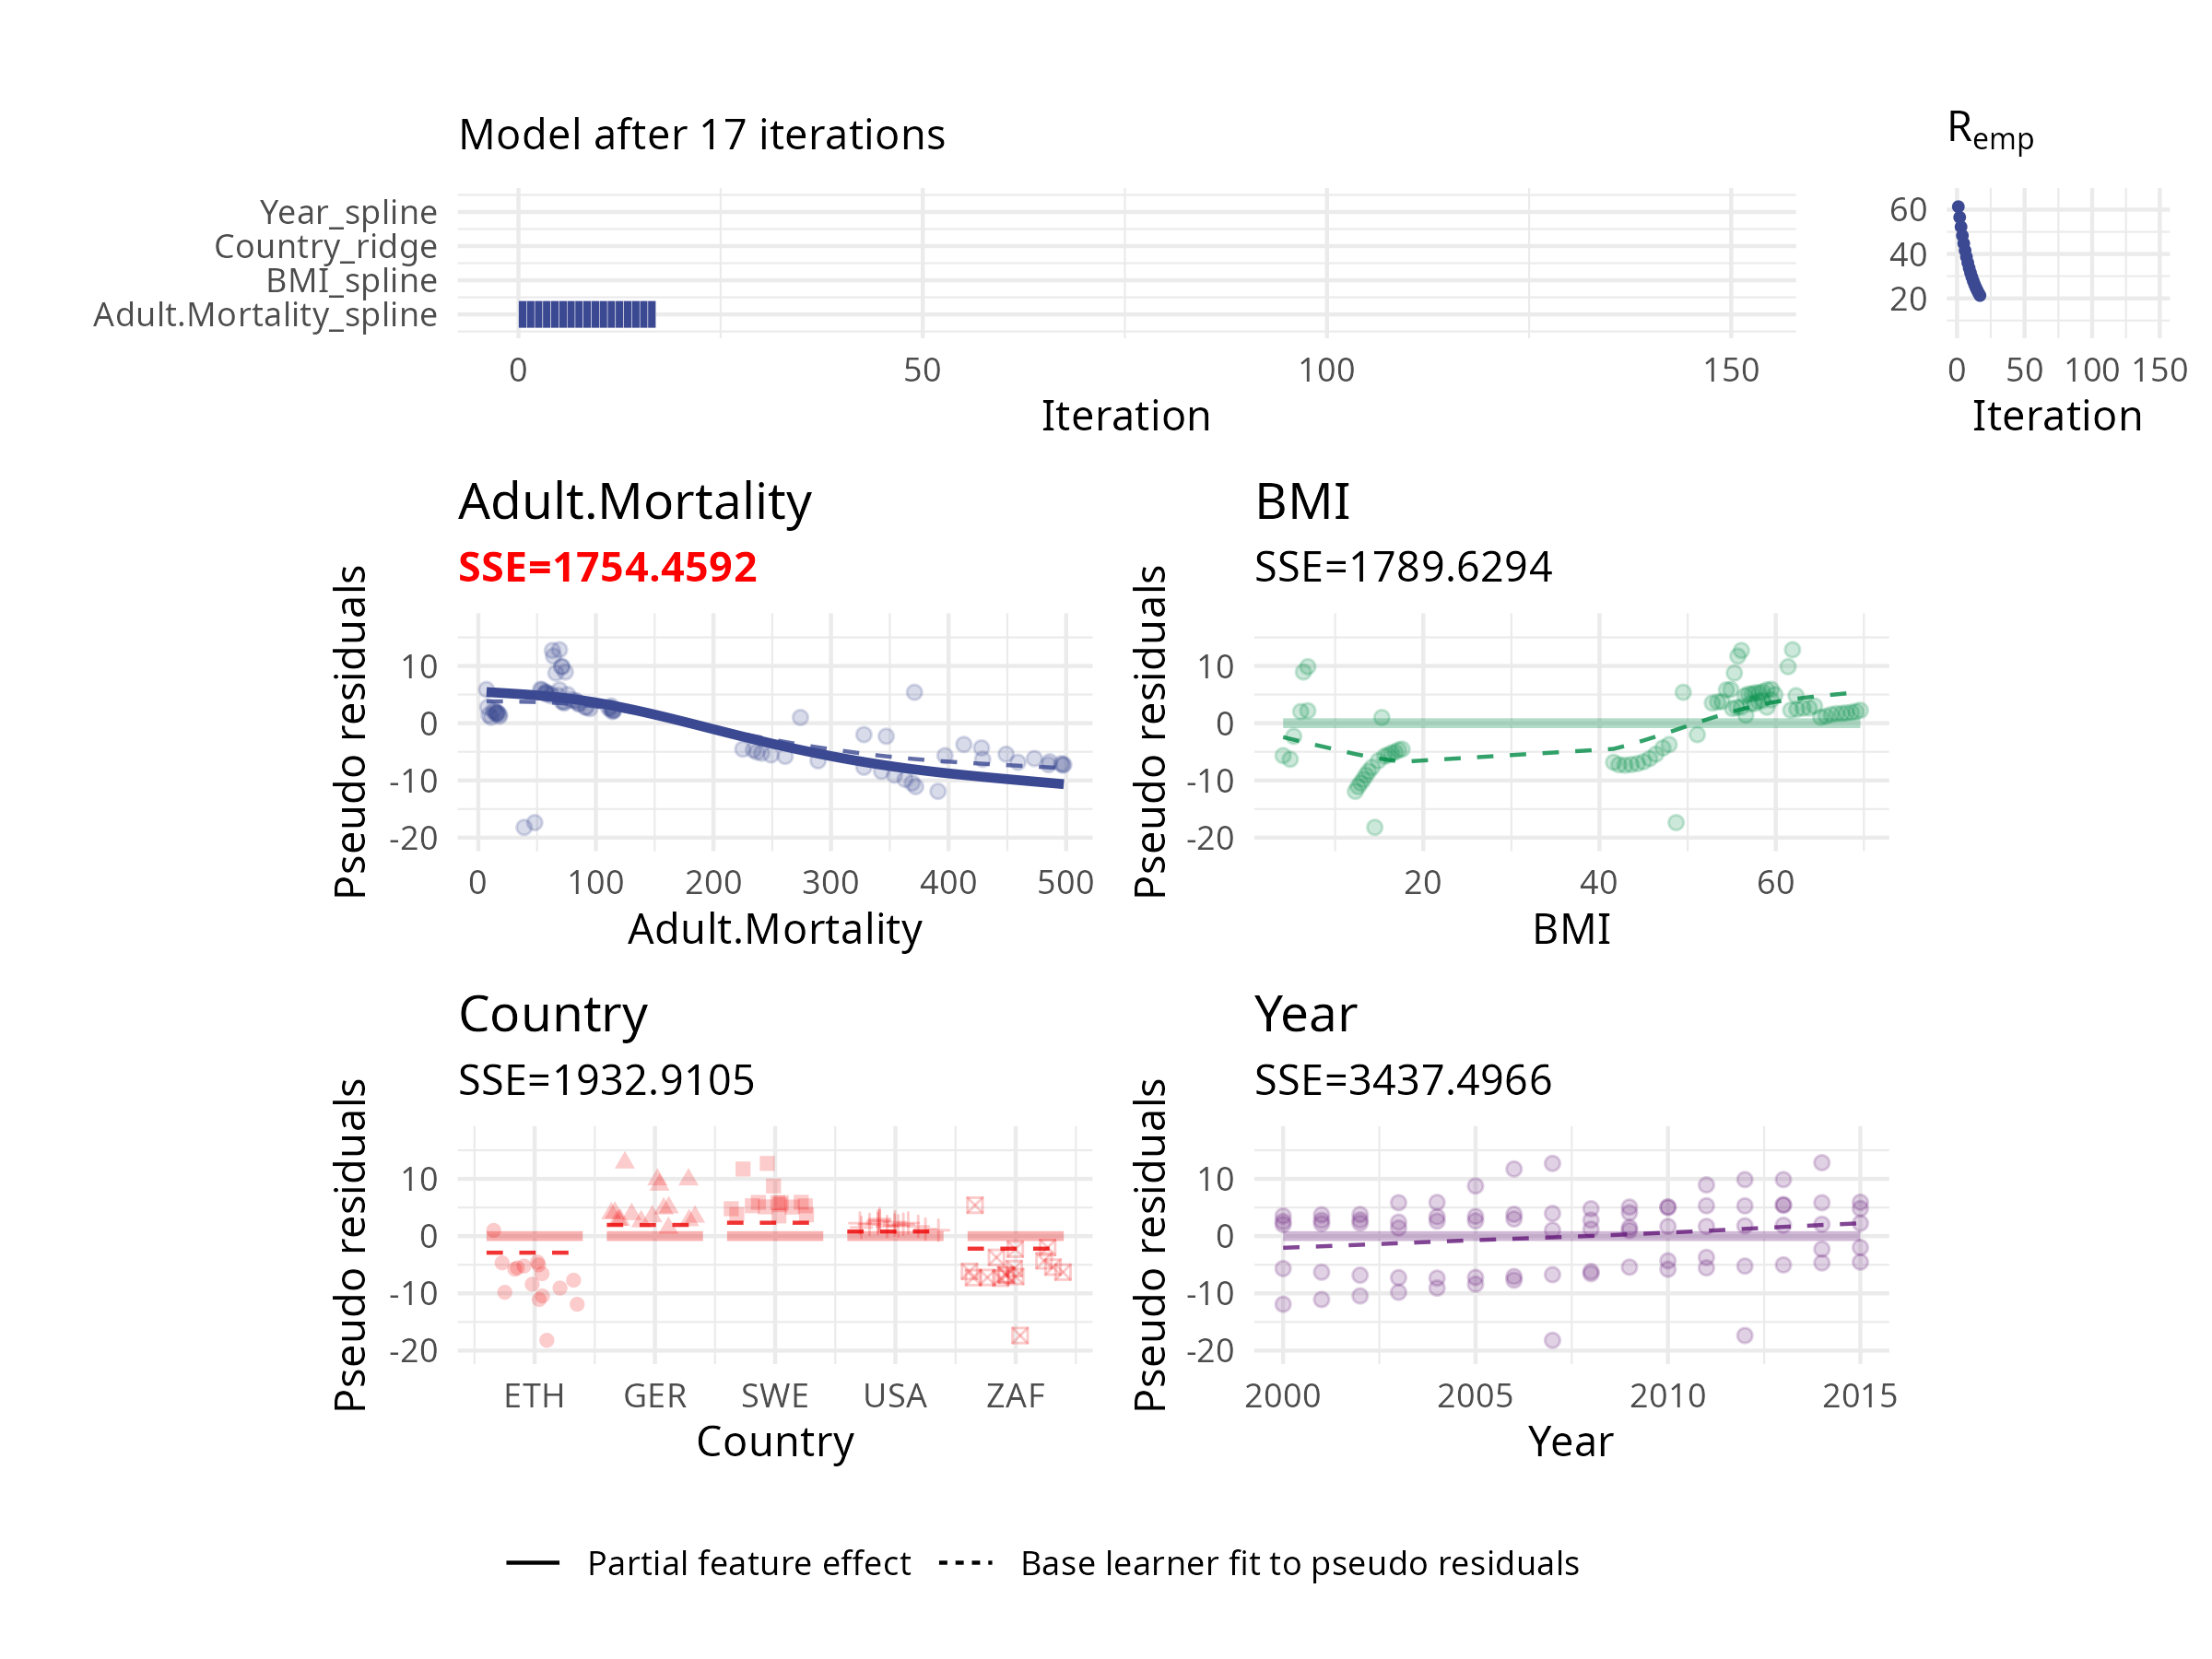
\includegraphics[width=\textwidth]{figures/cwb-anim/fig-iter-0017.png}
	\end{figure}
	\addtocounter{framenumber}{-1}
\end{frame}


\begin{frame}{Example: Life expectancy (nonlinear)}
	\begin{figure}
		\centering
		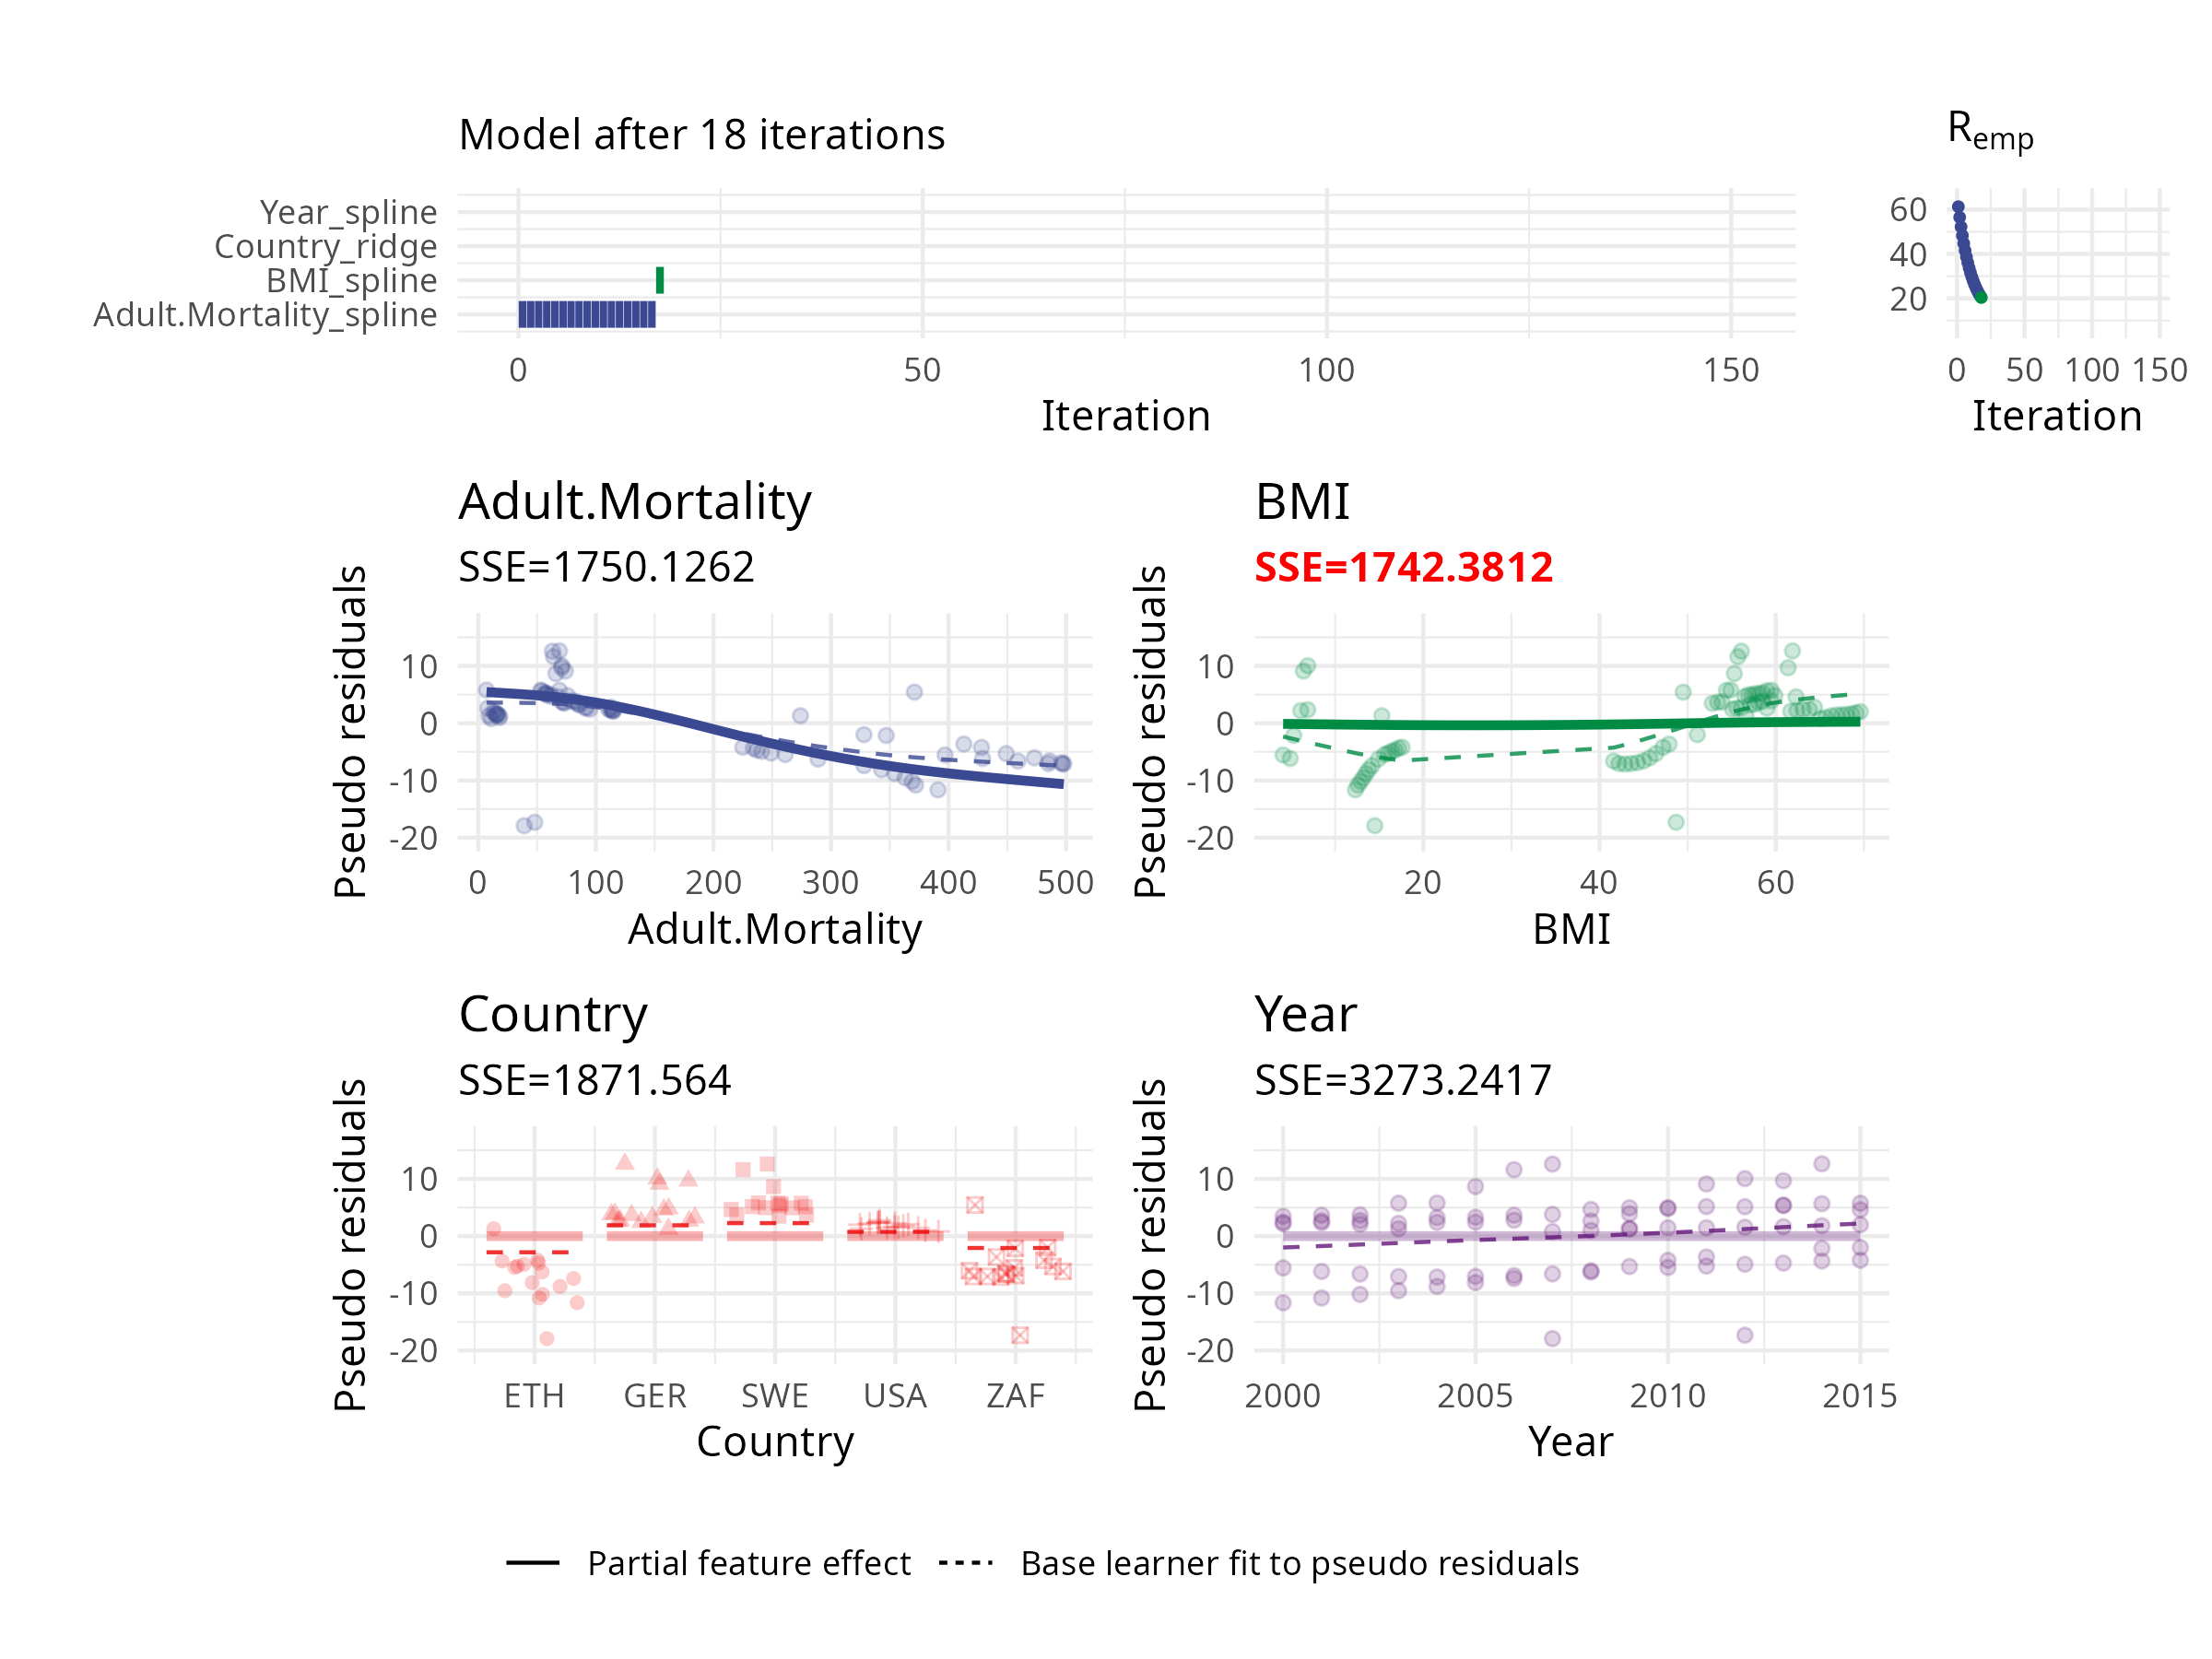
\includegraphics[width=\textwidth]{figures/cwb-anim/fig-iter-0018.png}
	\end{figure}
	\addtocounter{framenumber}{-1}
\end{frame}


\begin{frame}{Example: Life expectancy (nonlinear)}
	\begin{figure}
		\centering
		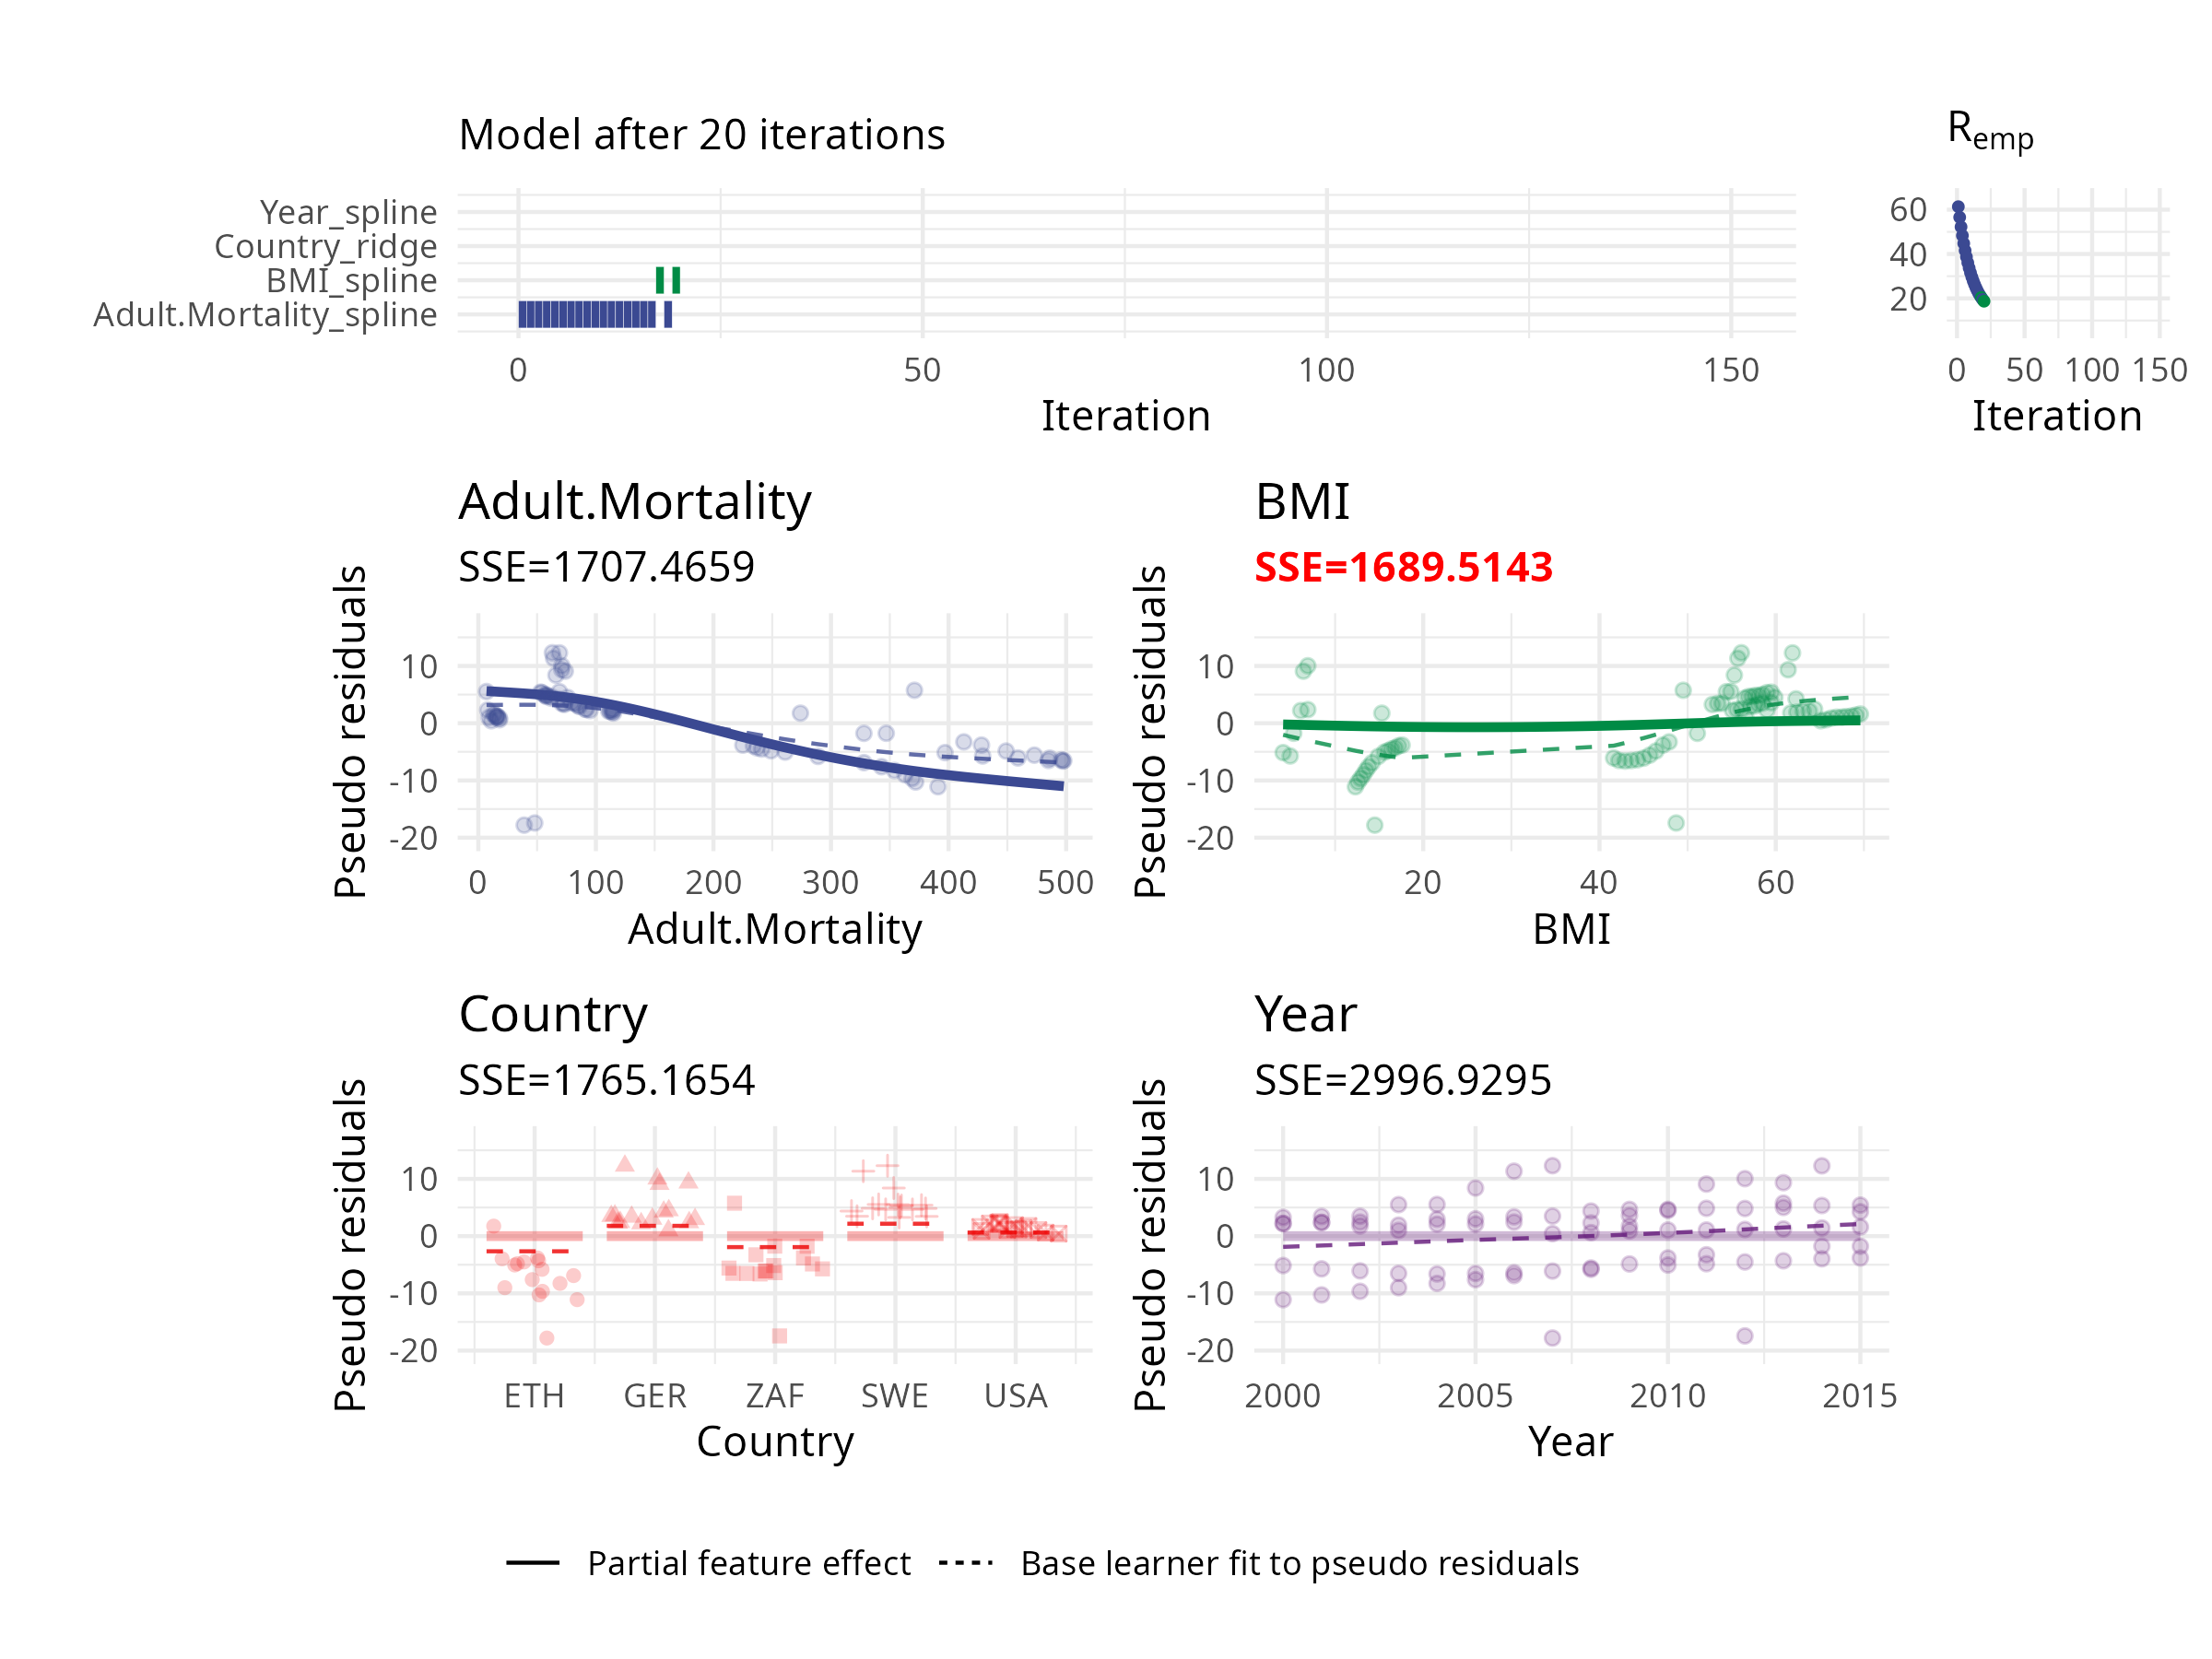
\includegraphics[width=\textwidth]{figures/cwb-anim/fig-iter-0020.png}
	\end{figure}
	\addtocounter{framenumber}{-1}
\end{frame}


\begin{frame}{Example: Life expectancy (nonlinear)}
	\begin{figure}
		\centering
		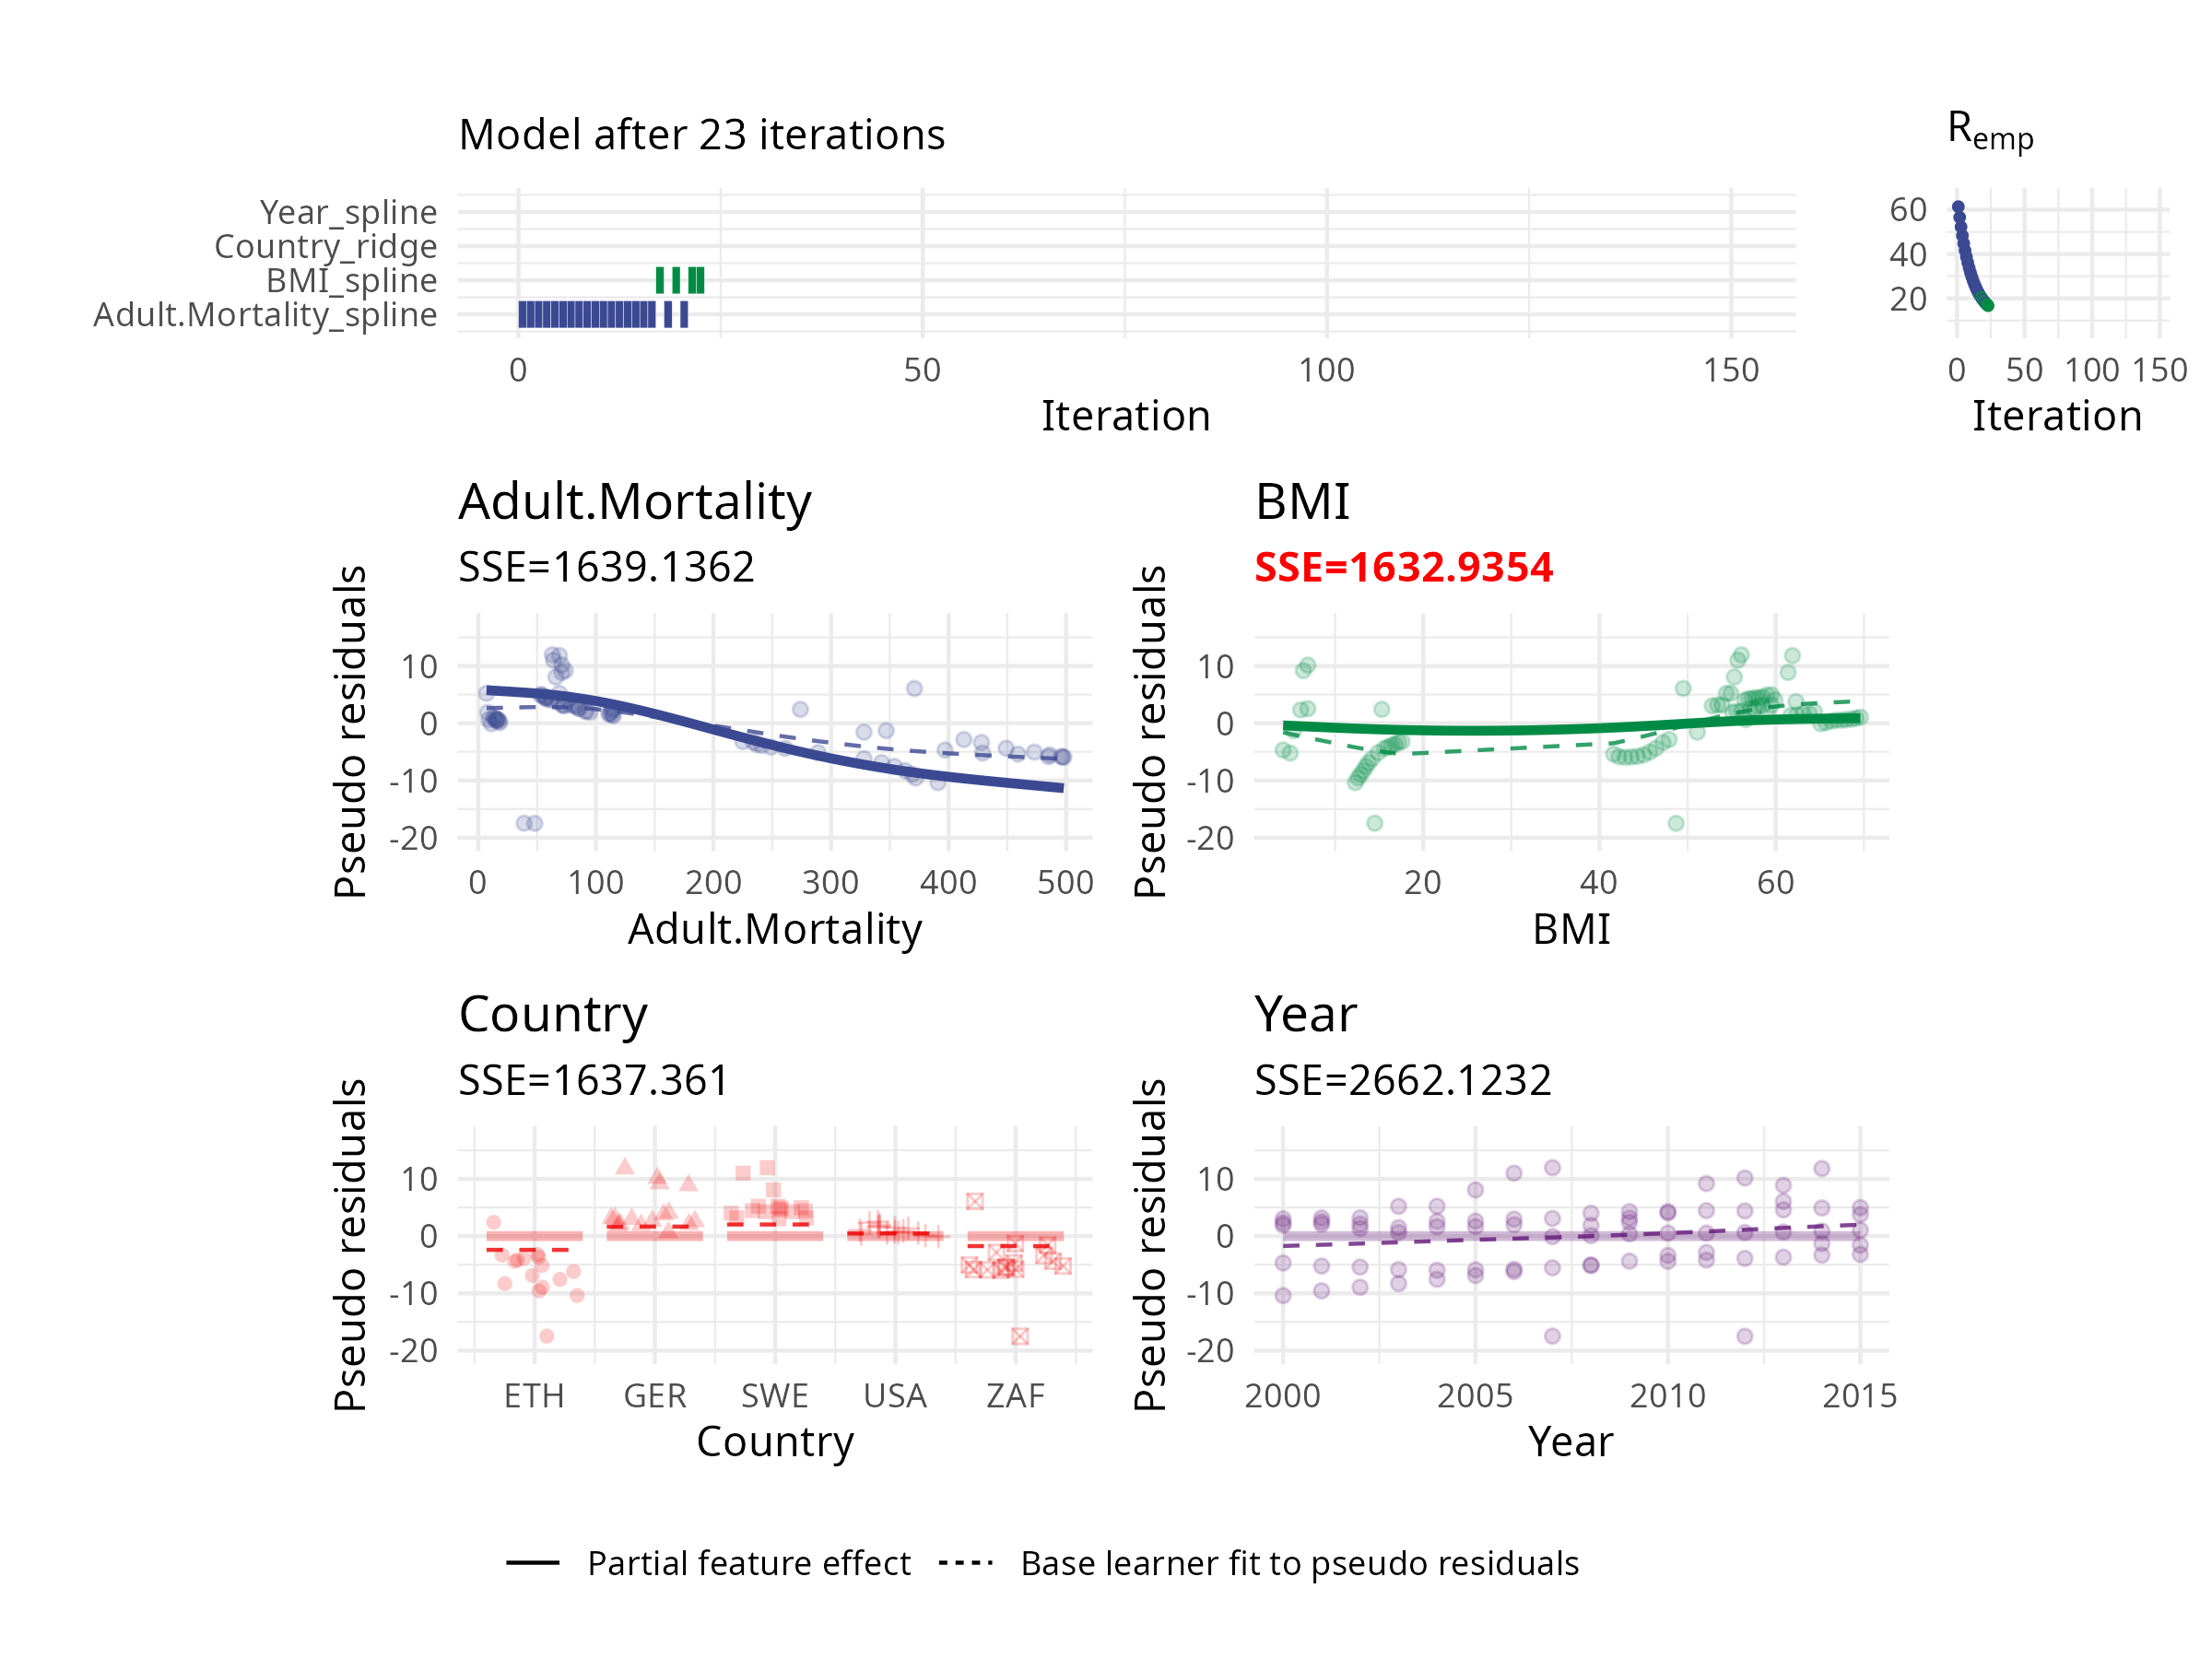
\includegraphics[width=\textwidth]{figures/cwb-anim/fig-iter-0023.png}
	\end{figure}
	\addtocounter{framenumber}{-1}
\end{frame}


\begin{frame}{Example: Life expectancy (nonlinear)}
	\begin{figure}
		\centering
		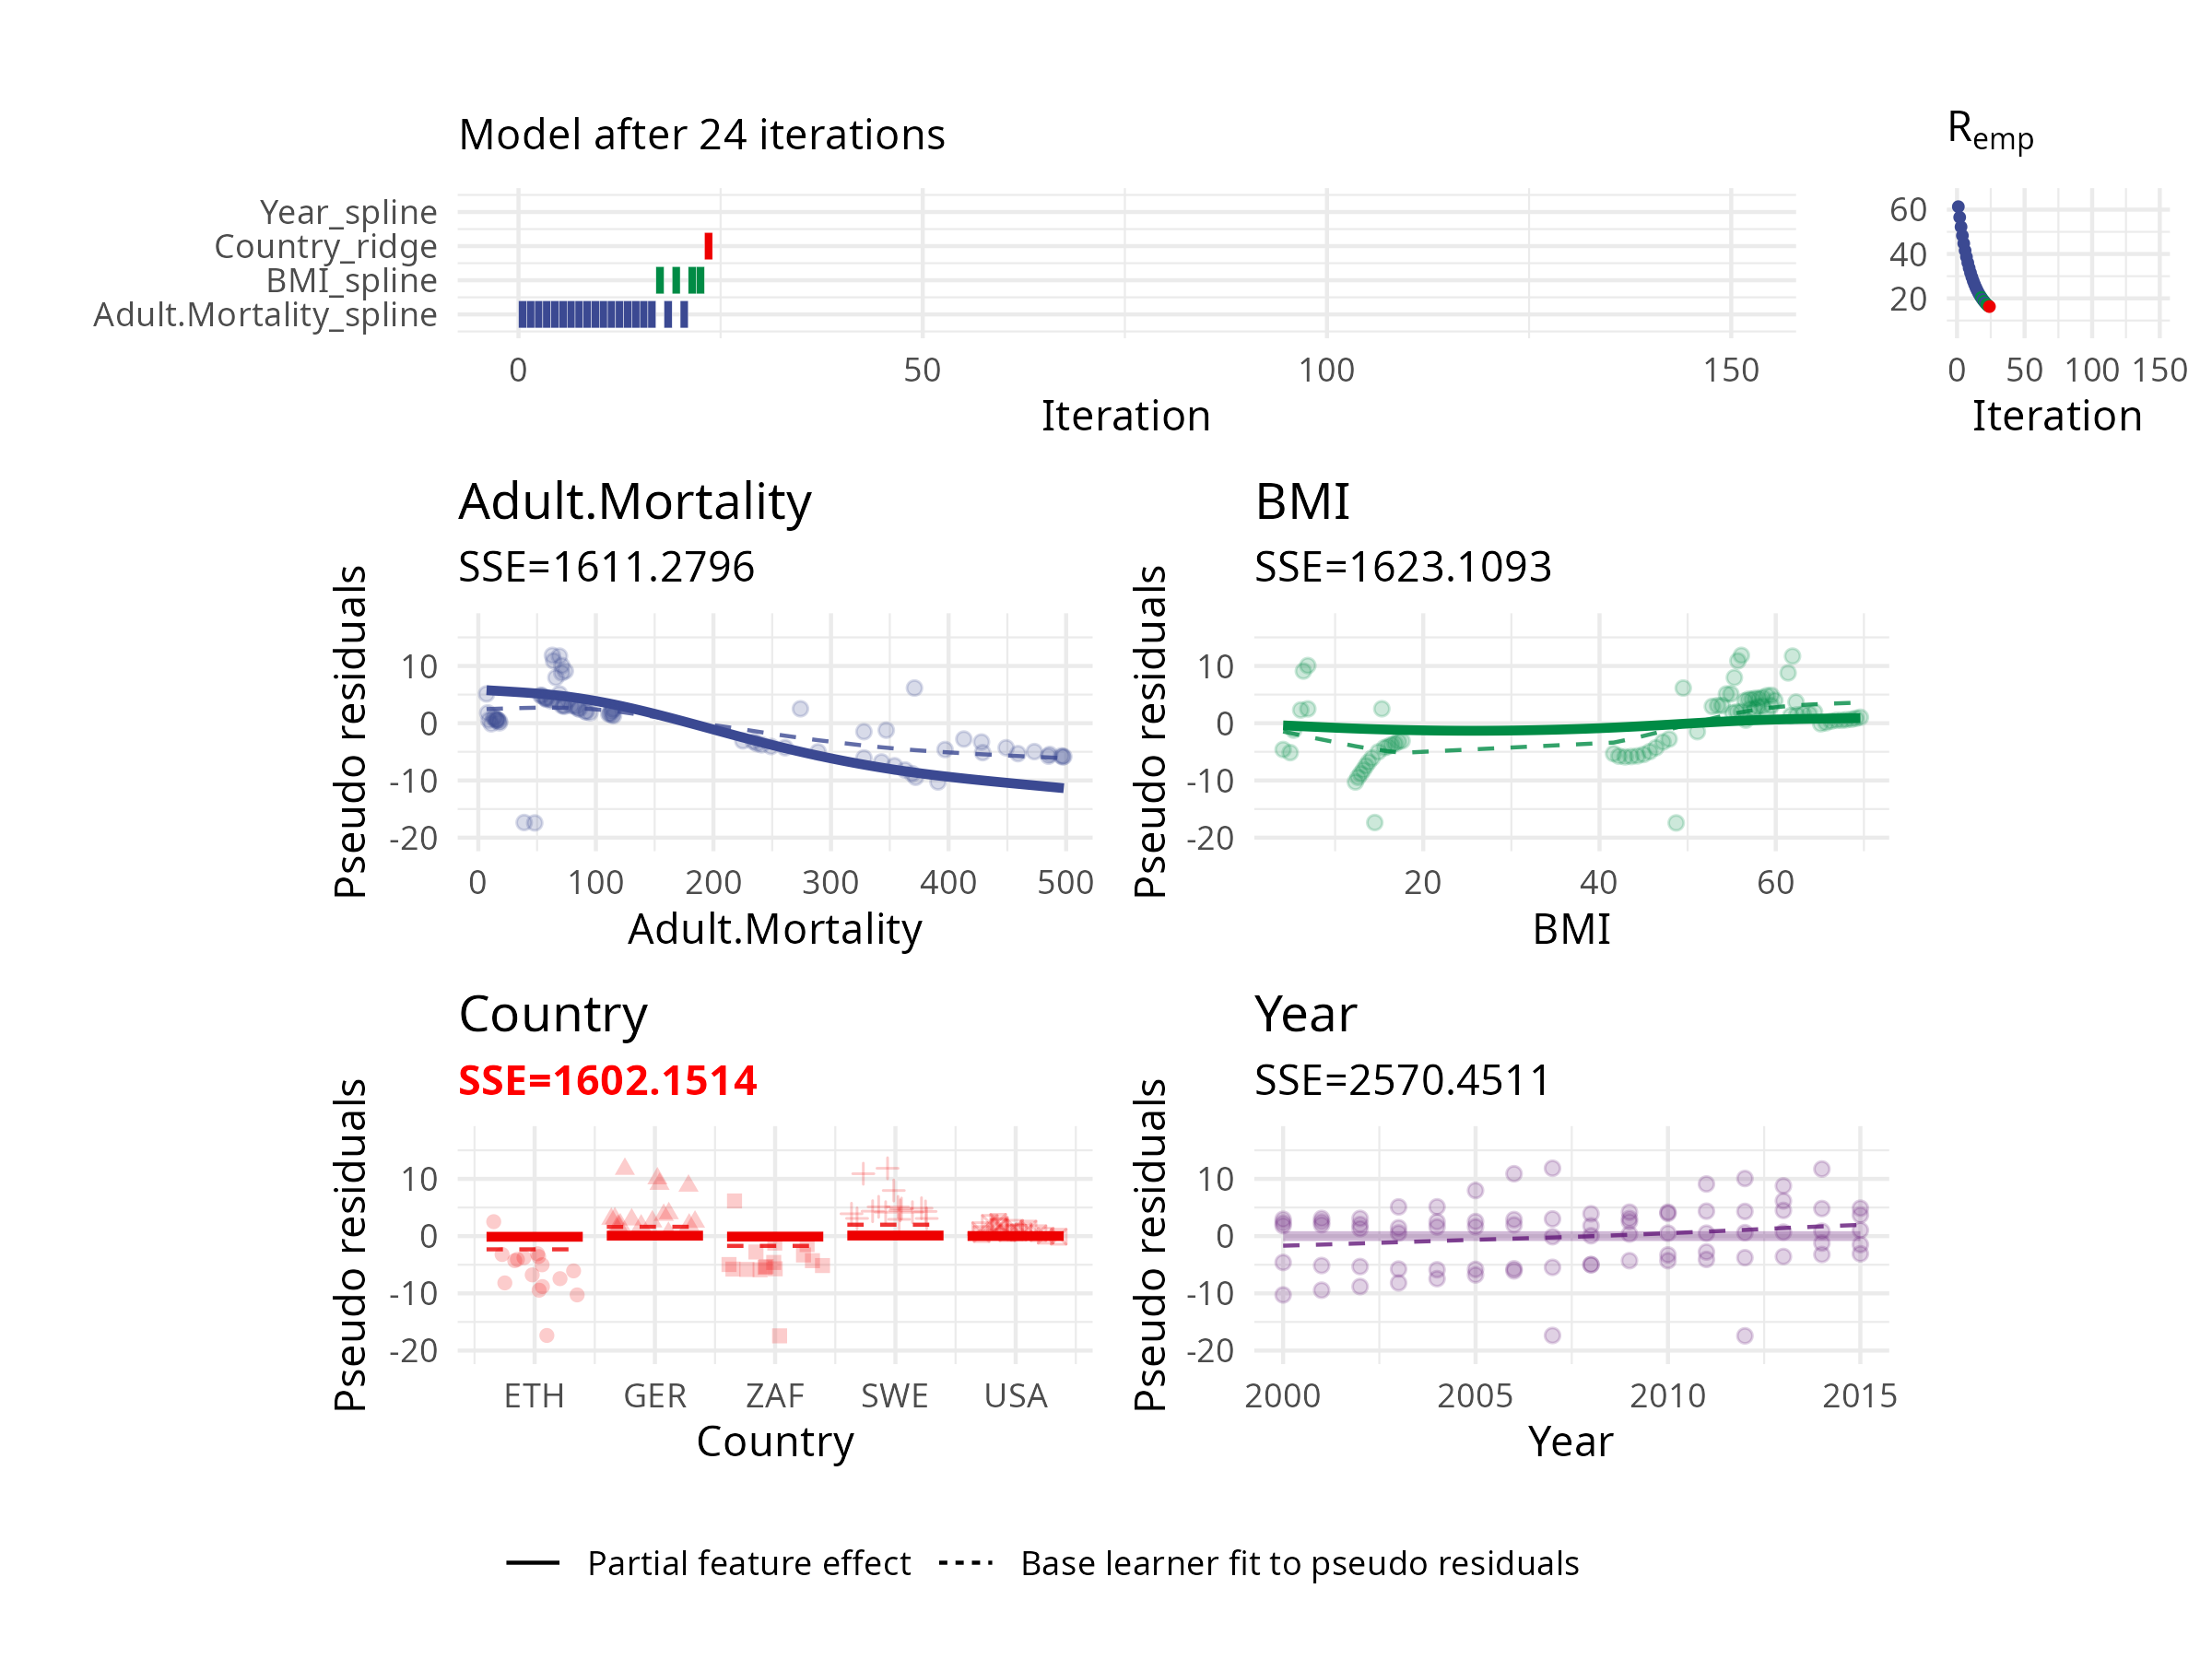
\includegraphics[width=\textwidth]{figures/cwb-anim/fig-iter-0024.png}
	\end{figure}
	\addtocounter{framenumber}{-1}
\end{frame}


\begin{frame}{Example: Life expectancy (nonlinear)}
	\begin{figure}
		\centering
		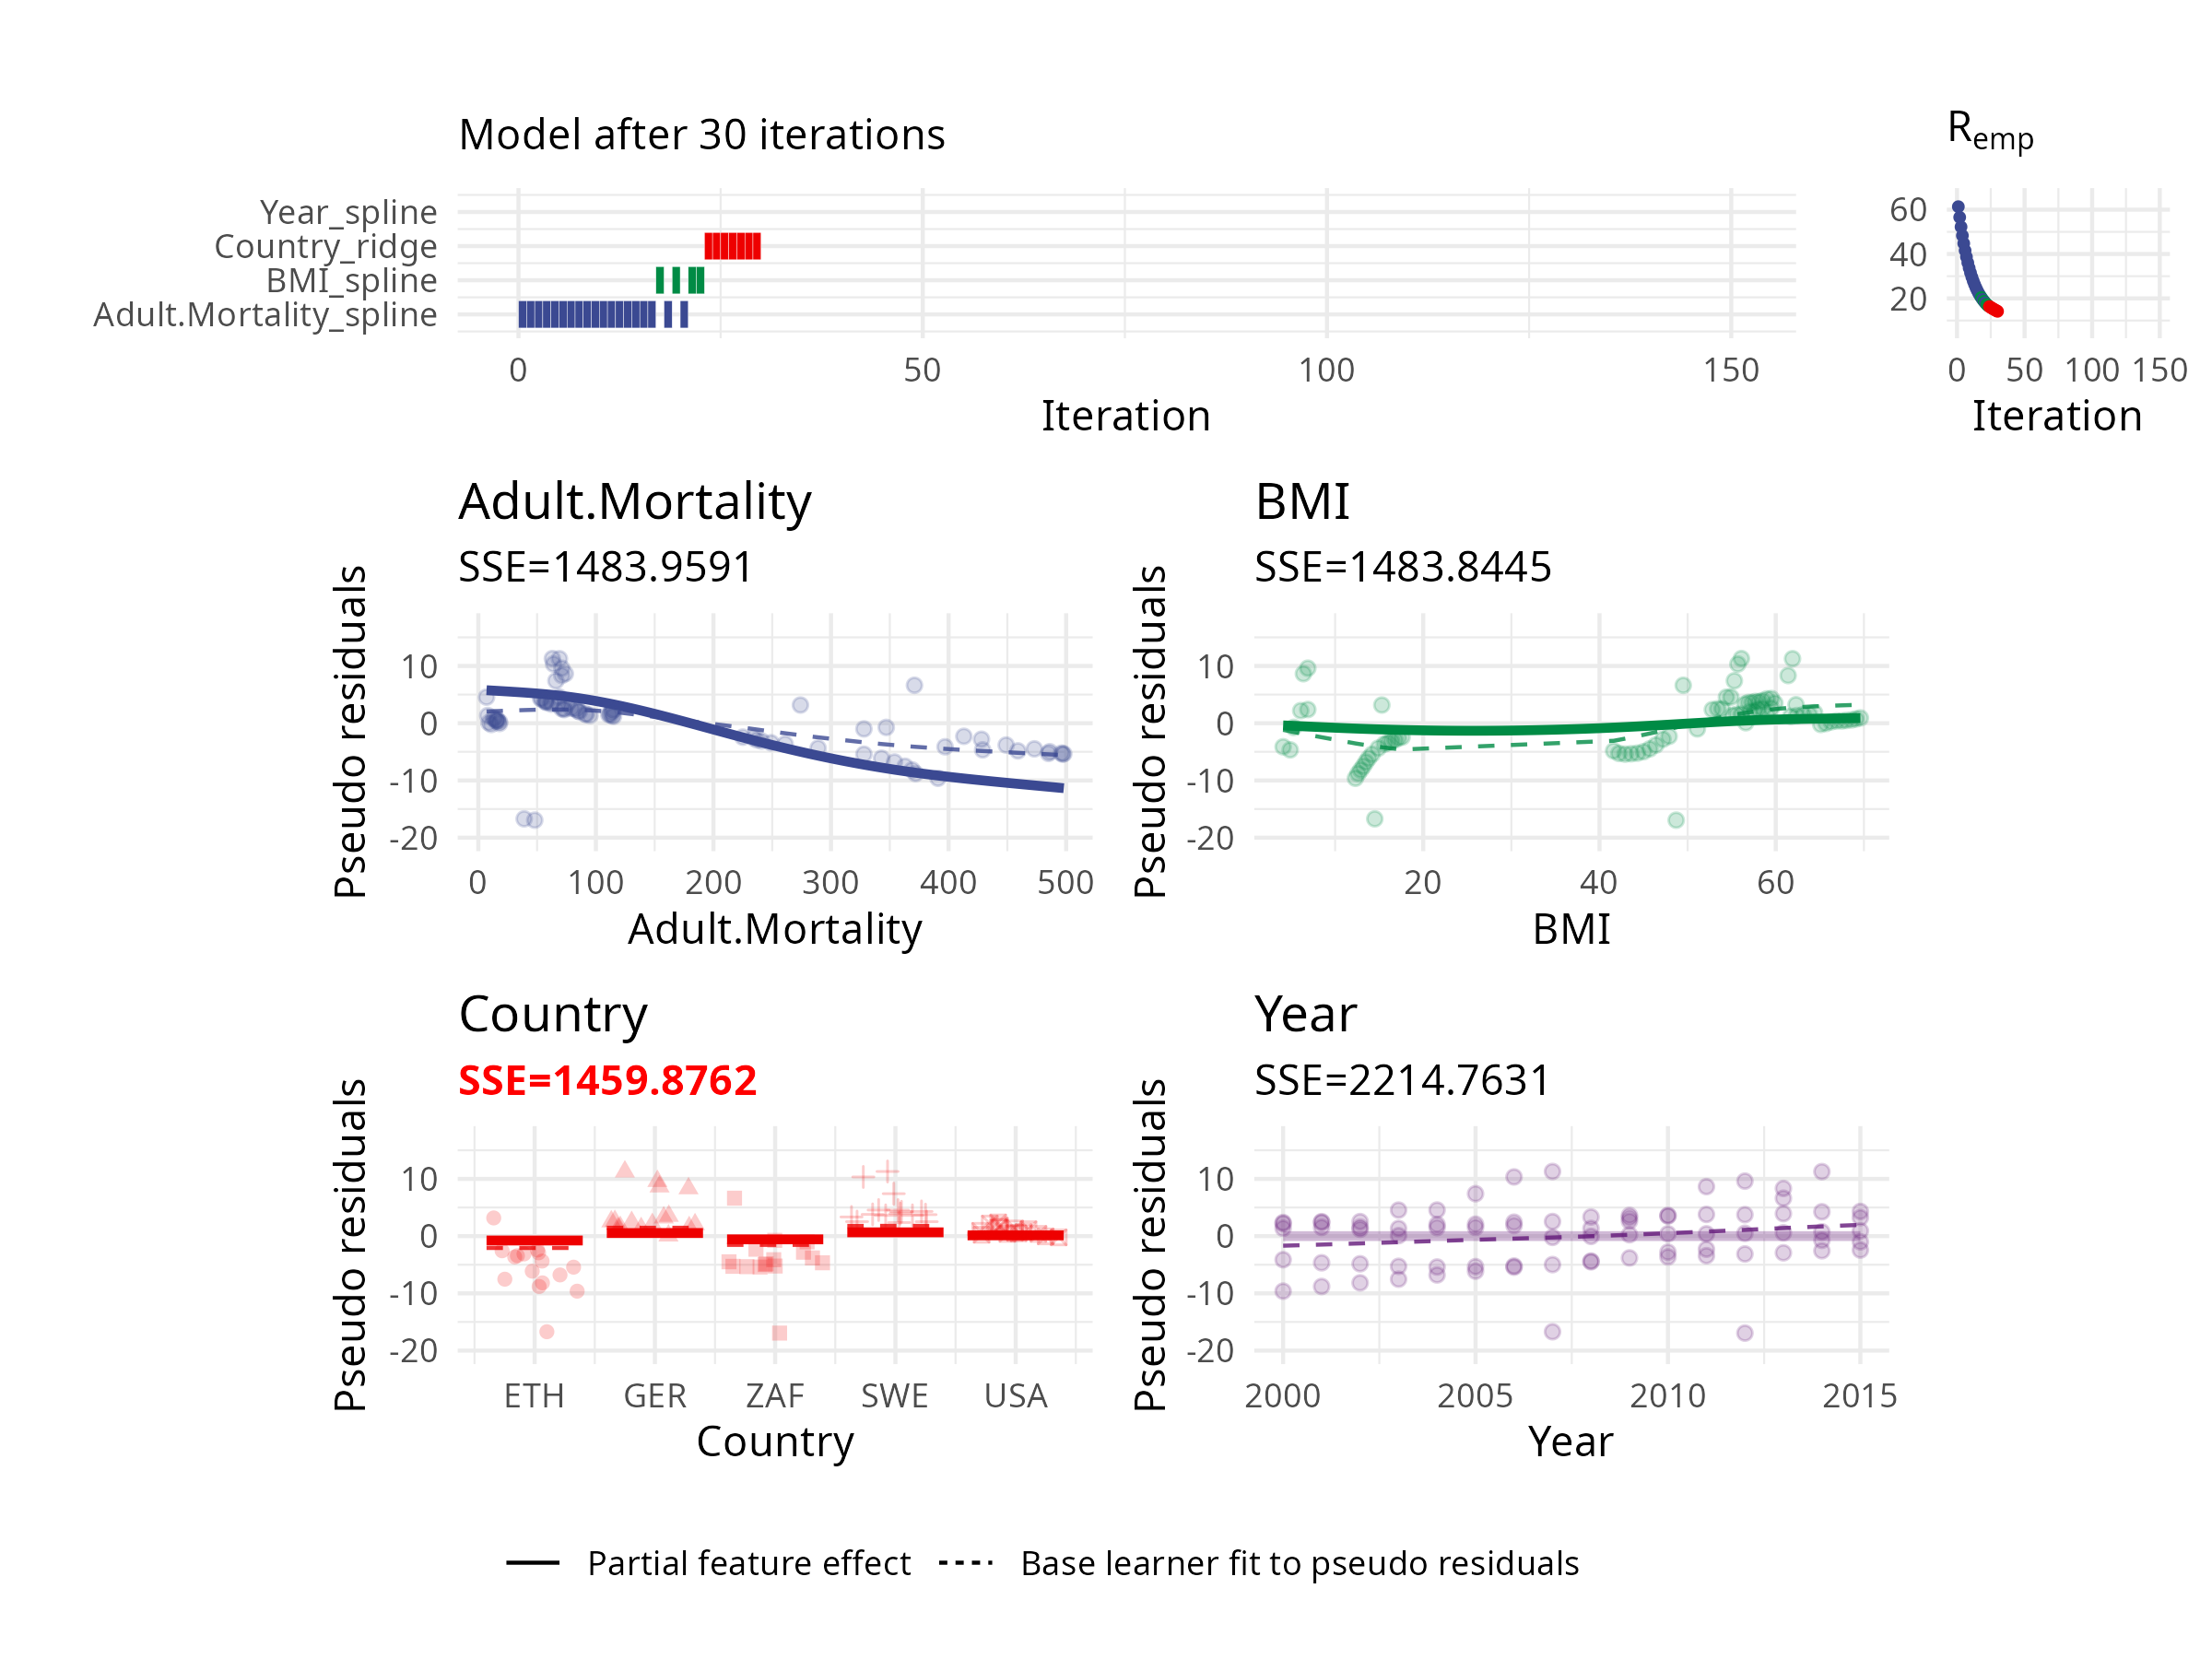
\includegraphics[width=\textwidth]{figures/cwb-anim/fig-iter-0030.png}
	\end{figure}
	\addtocounter{framenumber}{-1}
\end{frame}


\begin{frame}{Example: Life expectancy (nonlinear)}
	\begin{figure}
		\centering
		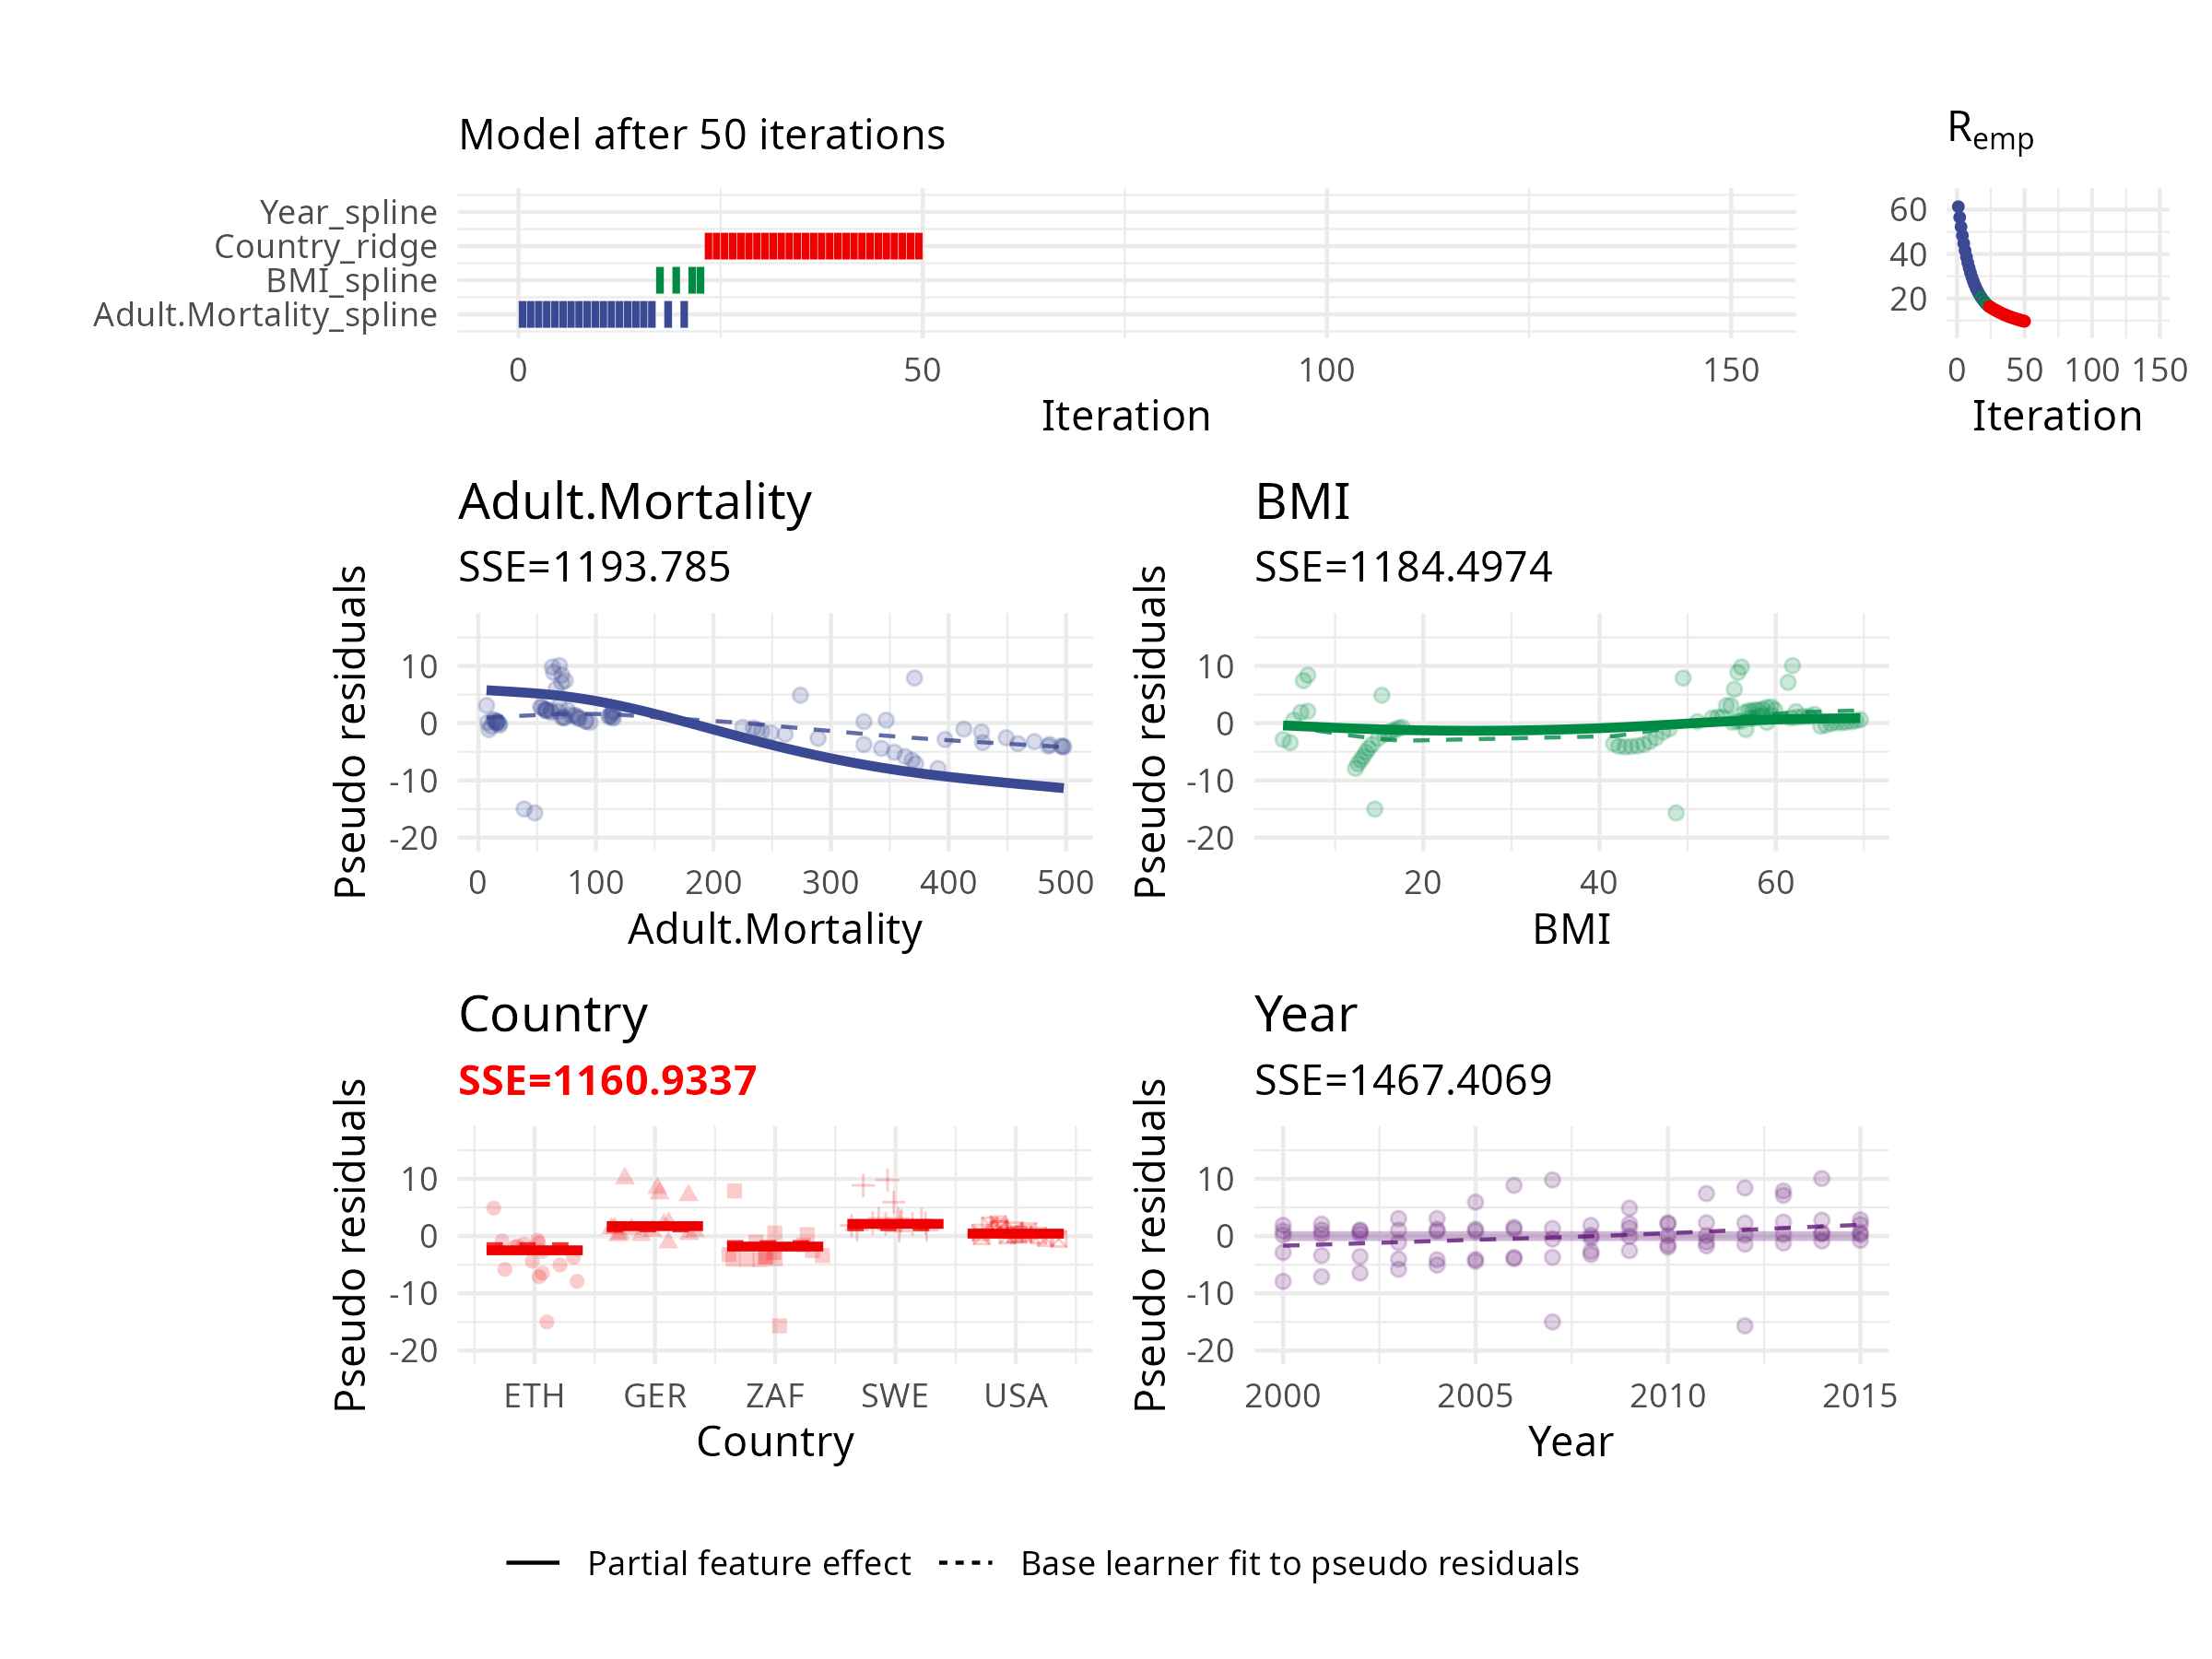
\includegraphics[width=\textwidth]{figures/cwb-anim/fig-iter-0050.png}
	\end{figure}
	\addtocounter{framenumber}{-1}
\end{frame}


\begin{frame}{Example: Life expectancy (nonlinear)}
	\begin{figure}
		\centering
		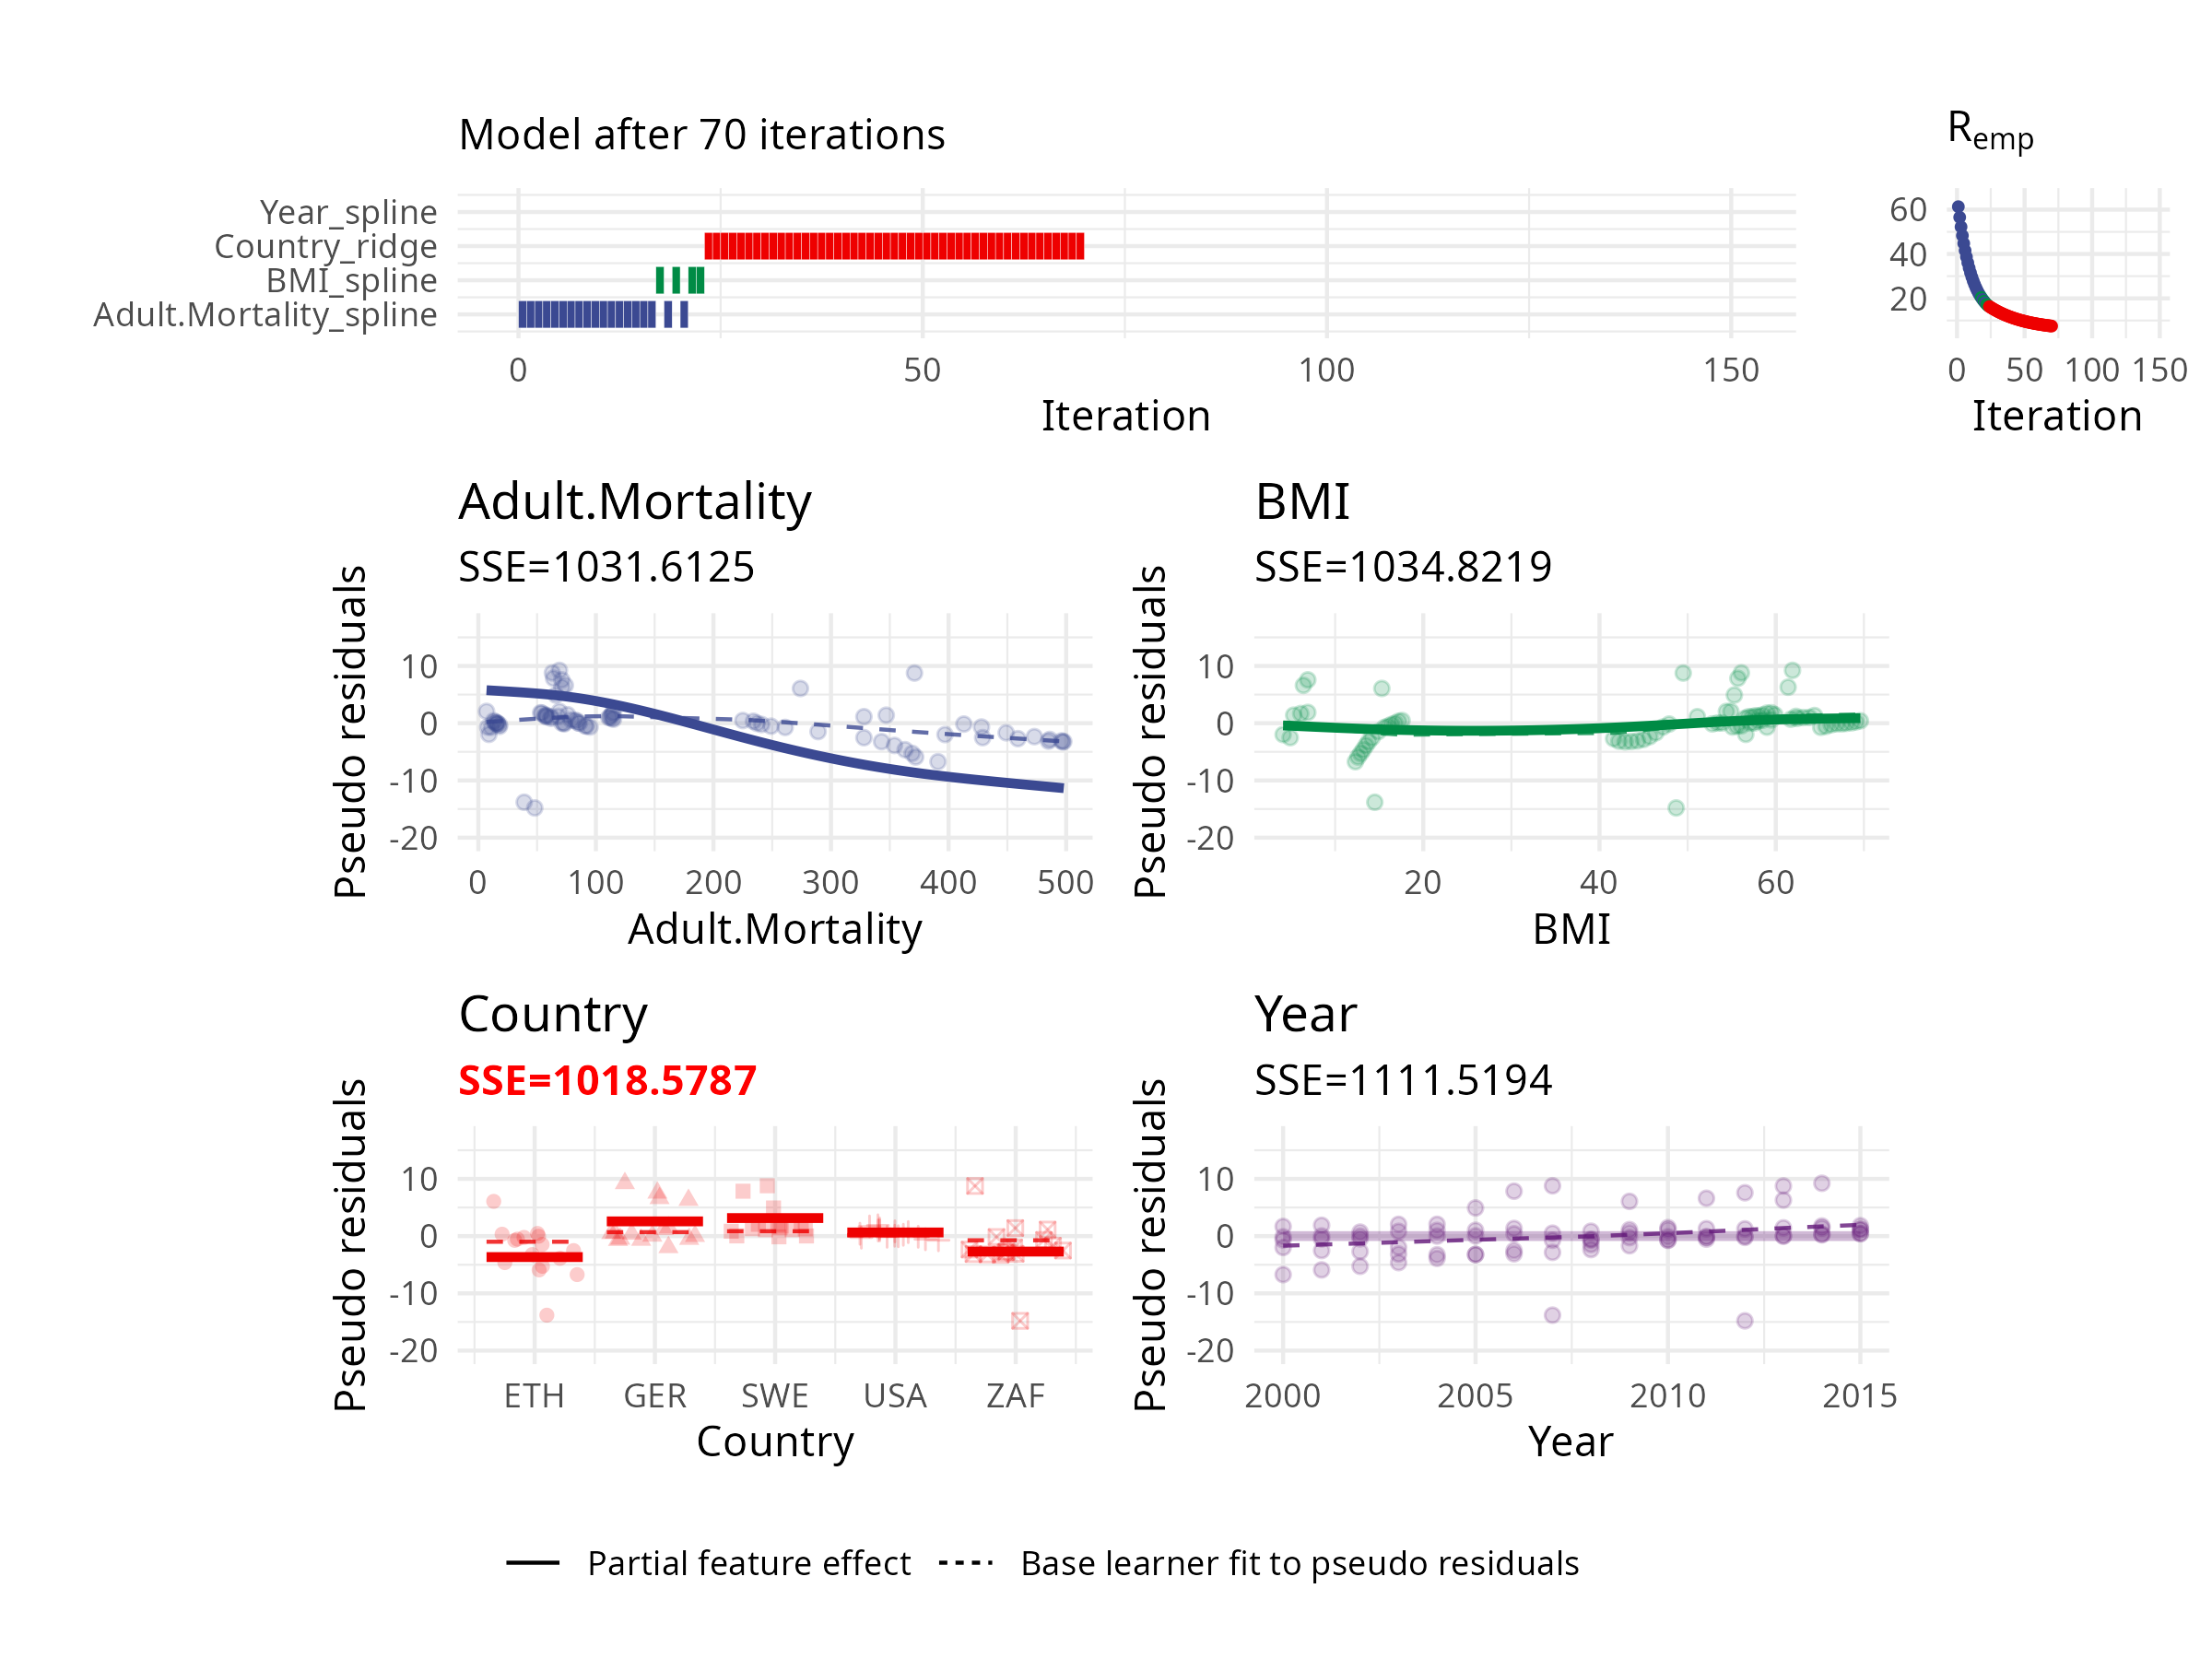
\includegraphics[width=\textwidth]{figures/cwb-anim/fig-iter-0070.png}
	\end{figure}
	\addtocounter{framenumber}{-1}
\end{frame}


\begin{frame}{Example: Life expectancy (nonlinear)}
	\begin{figure}
		\centering
		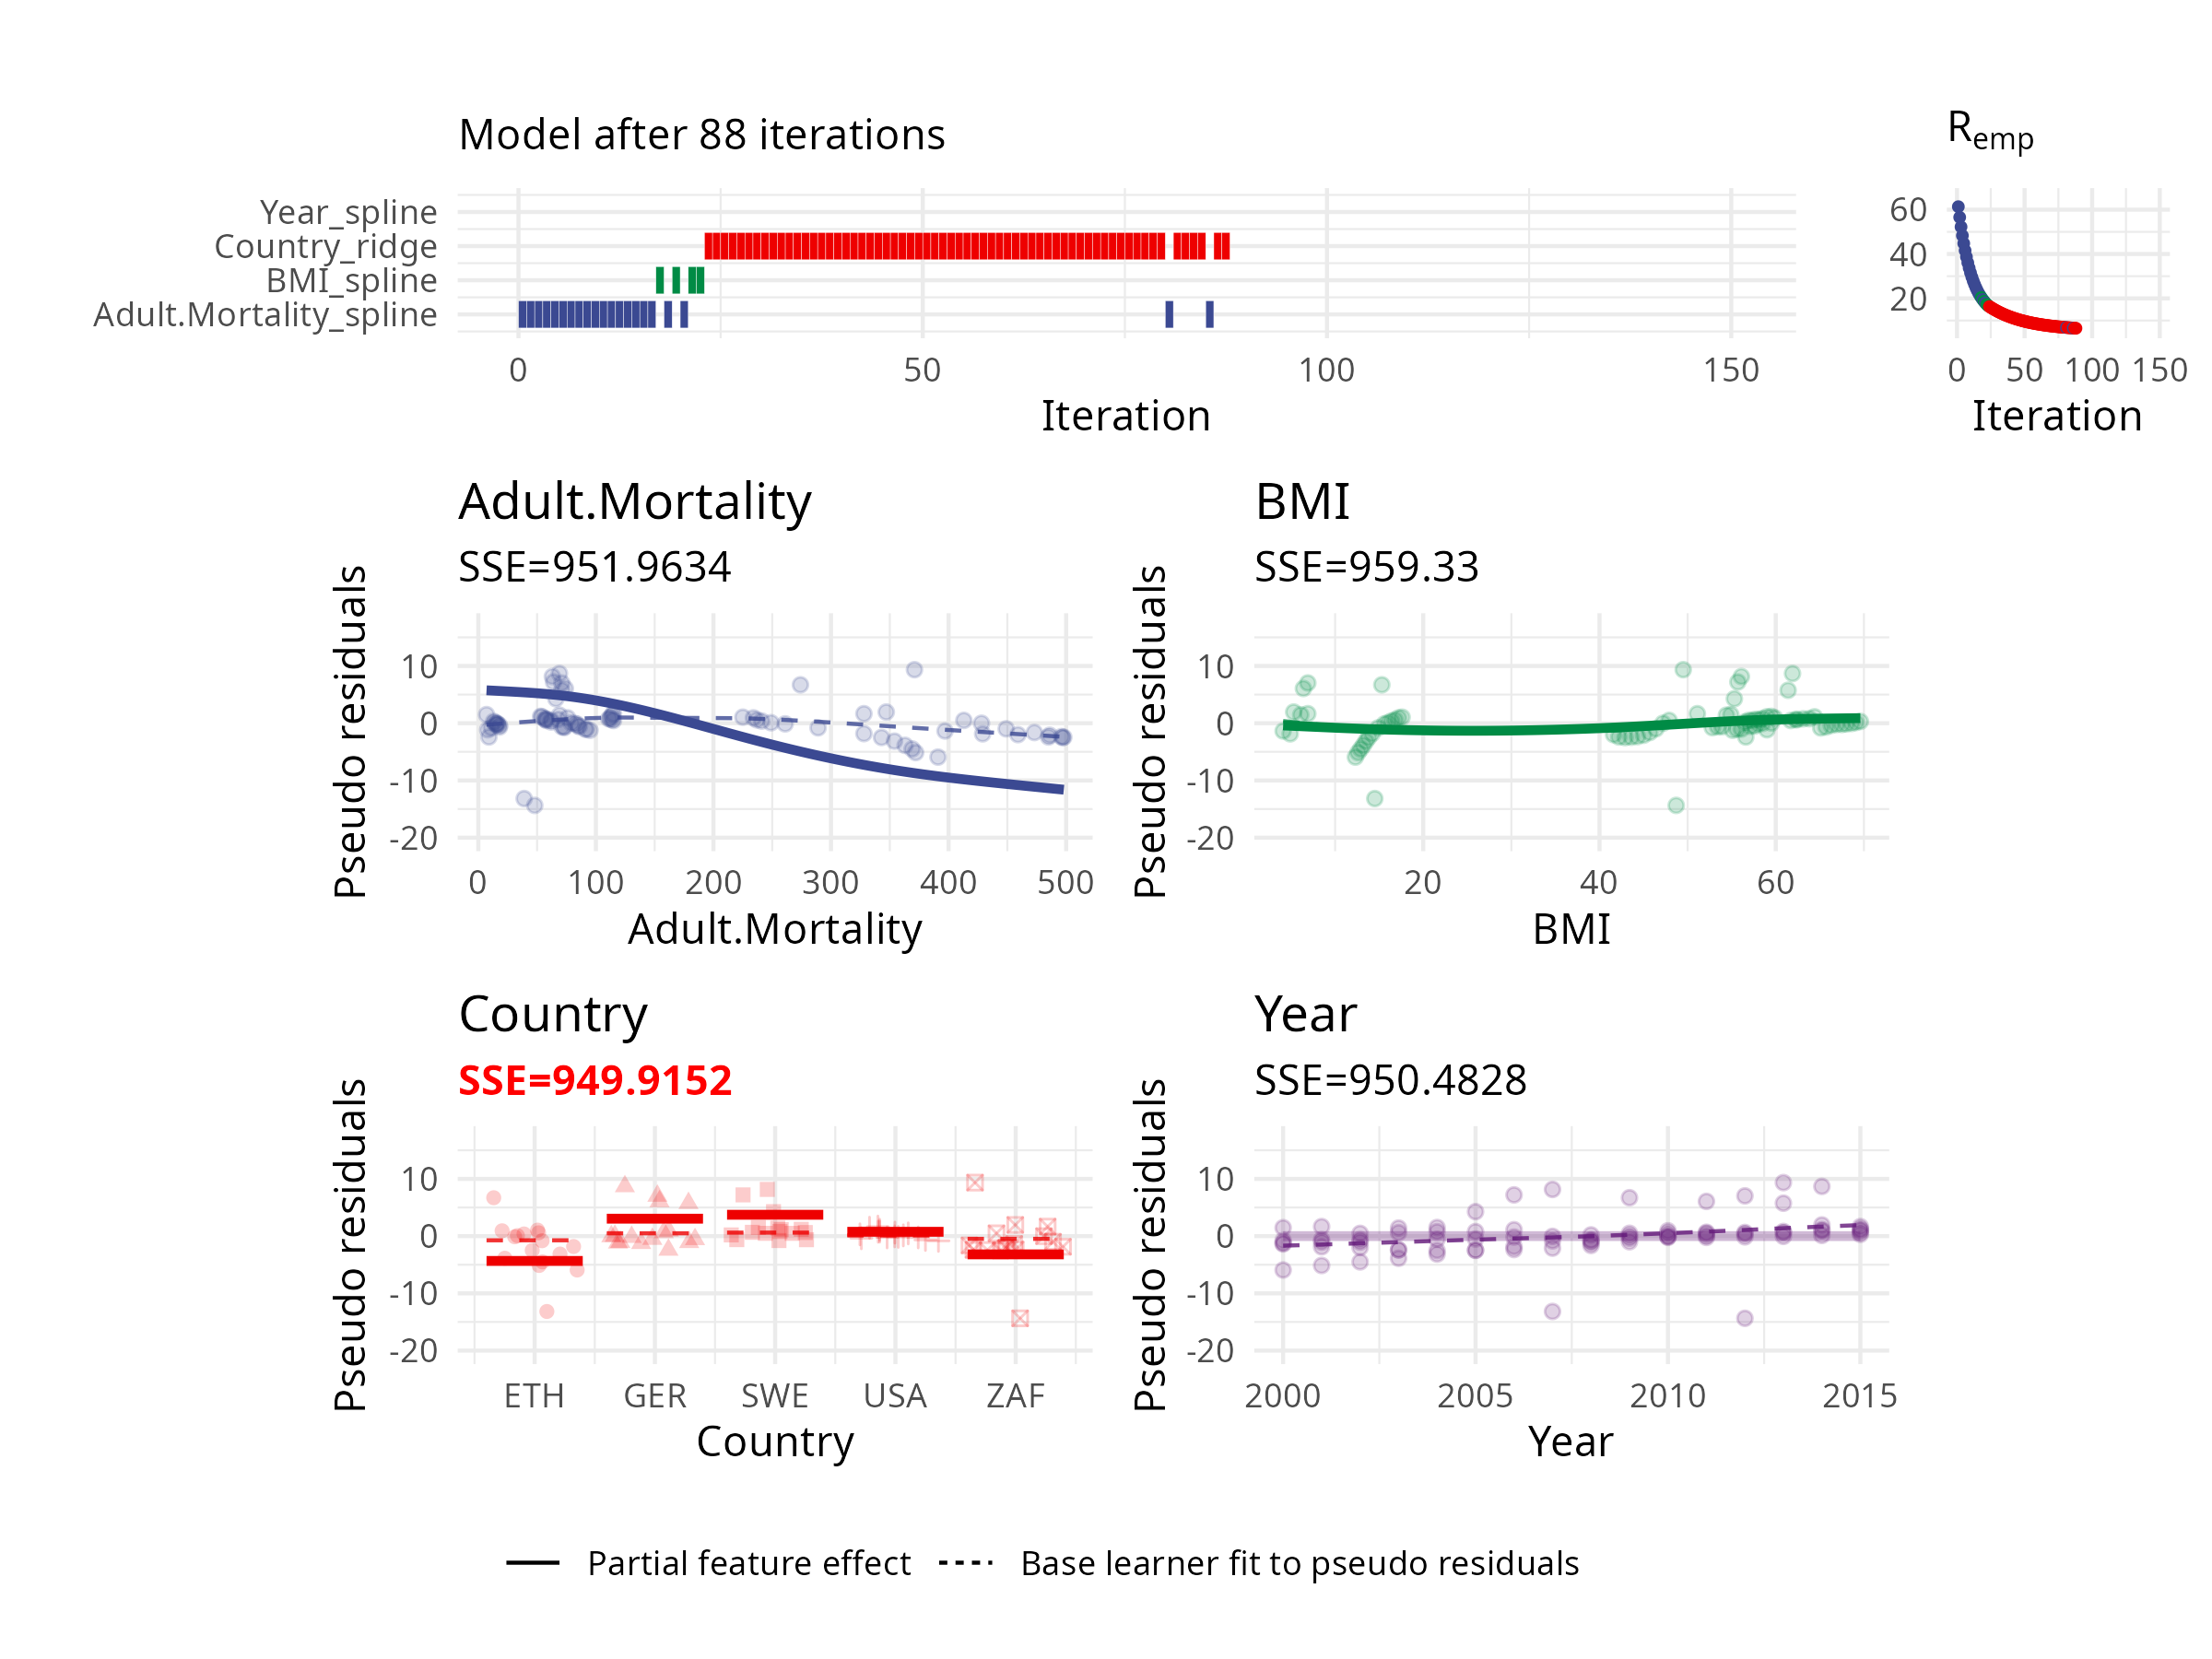
\includegraphics[width=\textwidth]{figures/cwb-anim/fig-iter-0088.png}
	\end{figure}
	\addtocounter{framenumber}{-1}
\end{frame}


\begin{frame}{Example: Life expectancy (nonlinear)}
	\begin{figure}
		\centering
		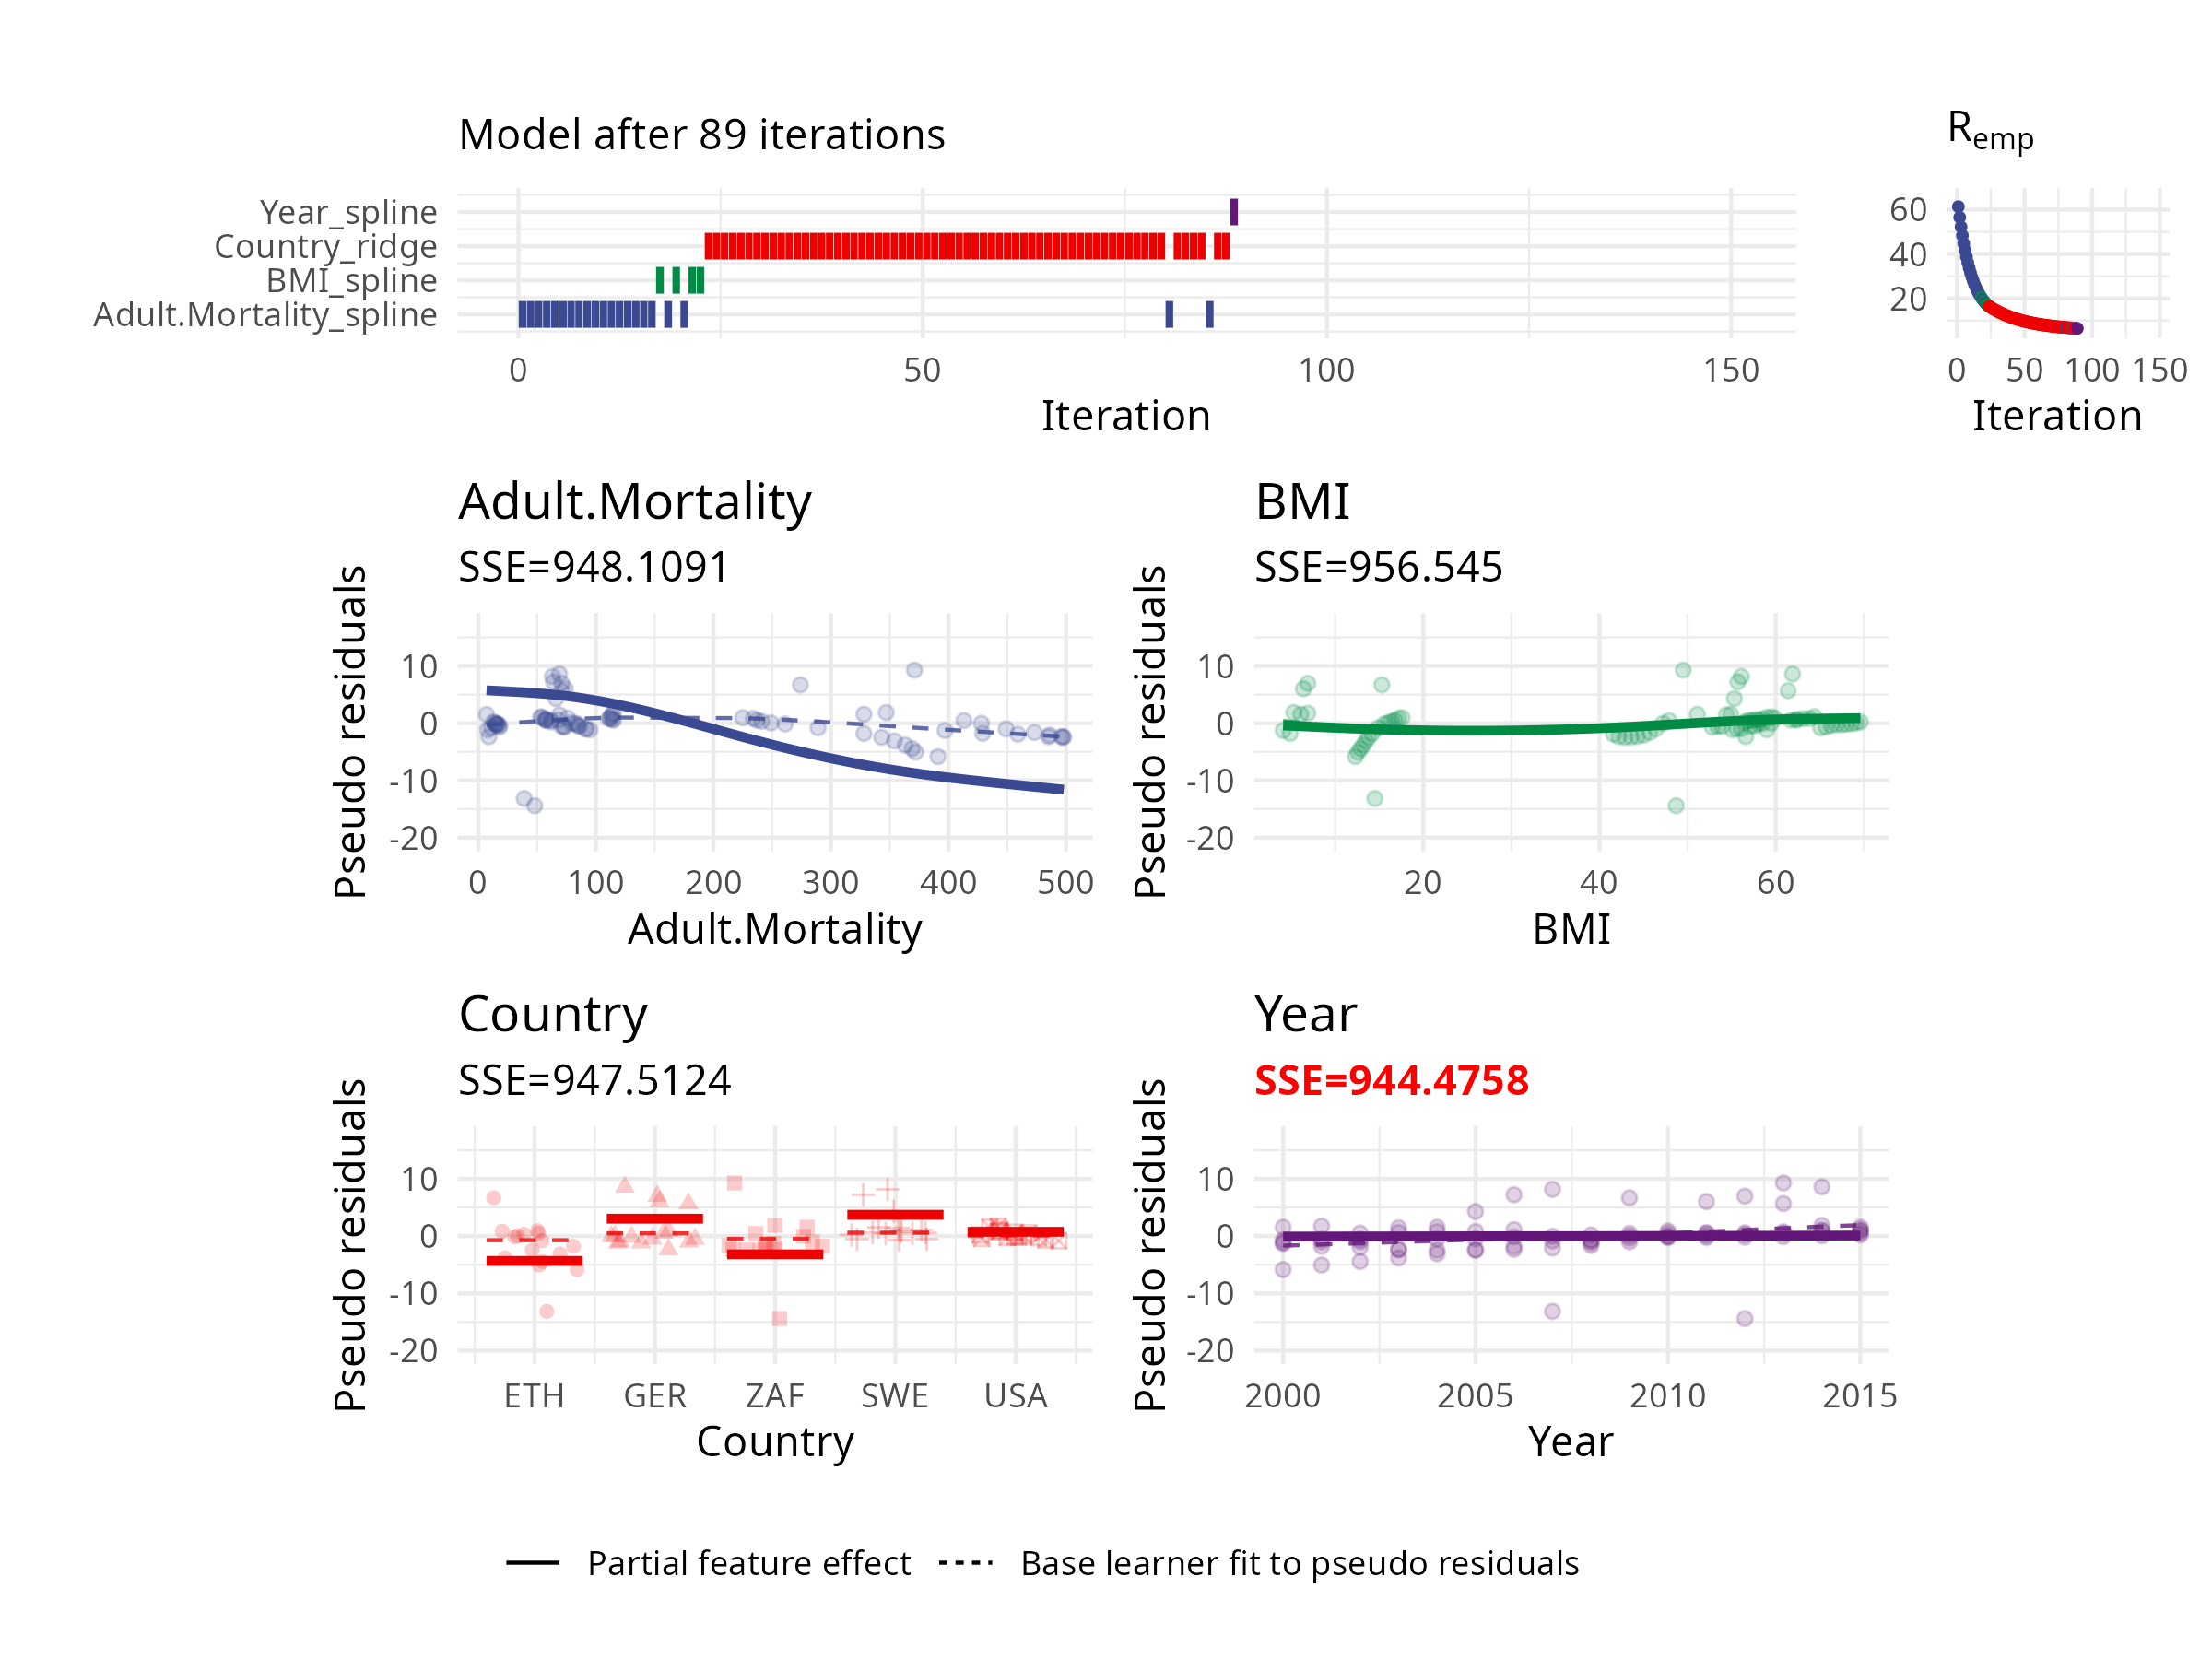
\includegraphics[width=\textwidth]{figures/cwb-anim/fig-iter-0089.png}
	\end{figure}
	\addtocounter{framenumber}{-1}
\end{frame}


\begin{frame}{Example: Life expectancy (nonlinear)}
	\begin{figure}
		\centering
		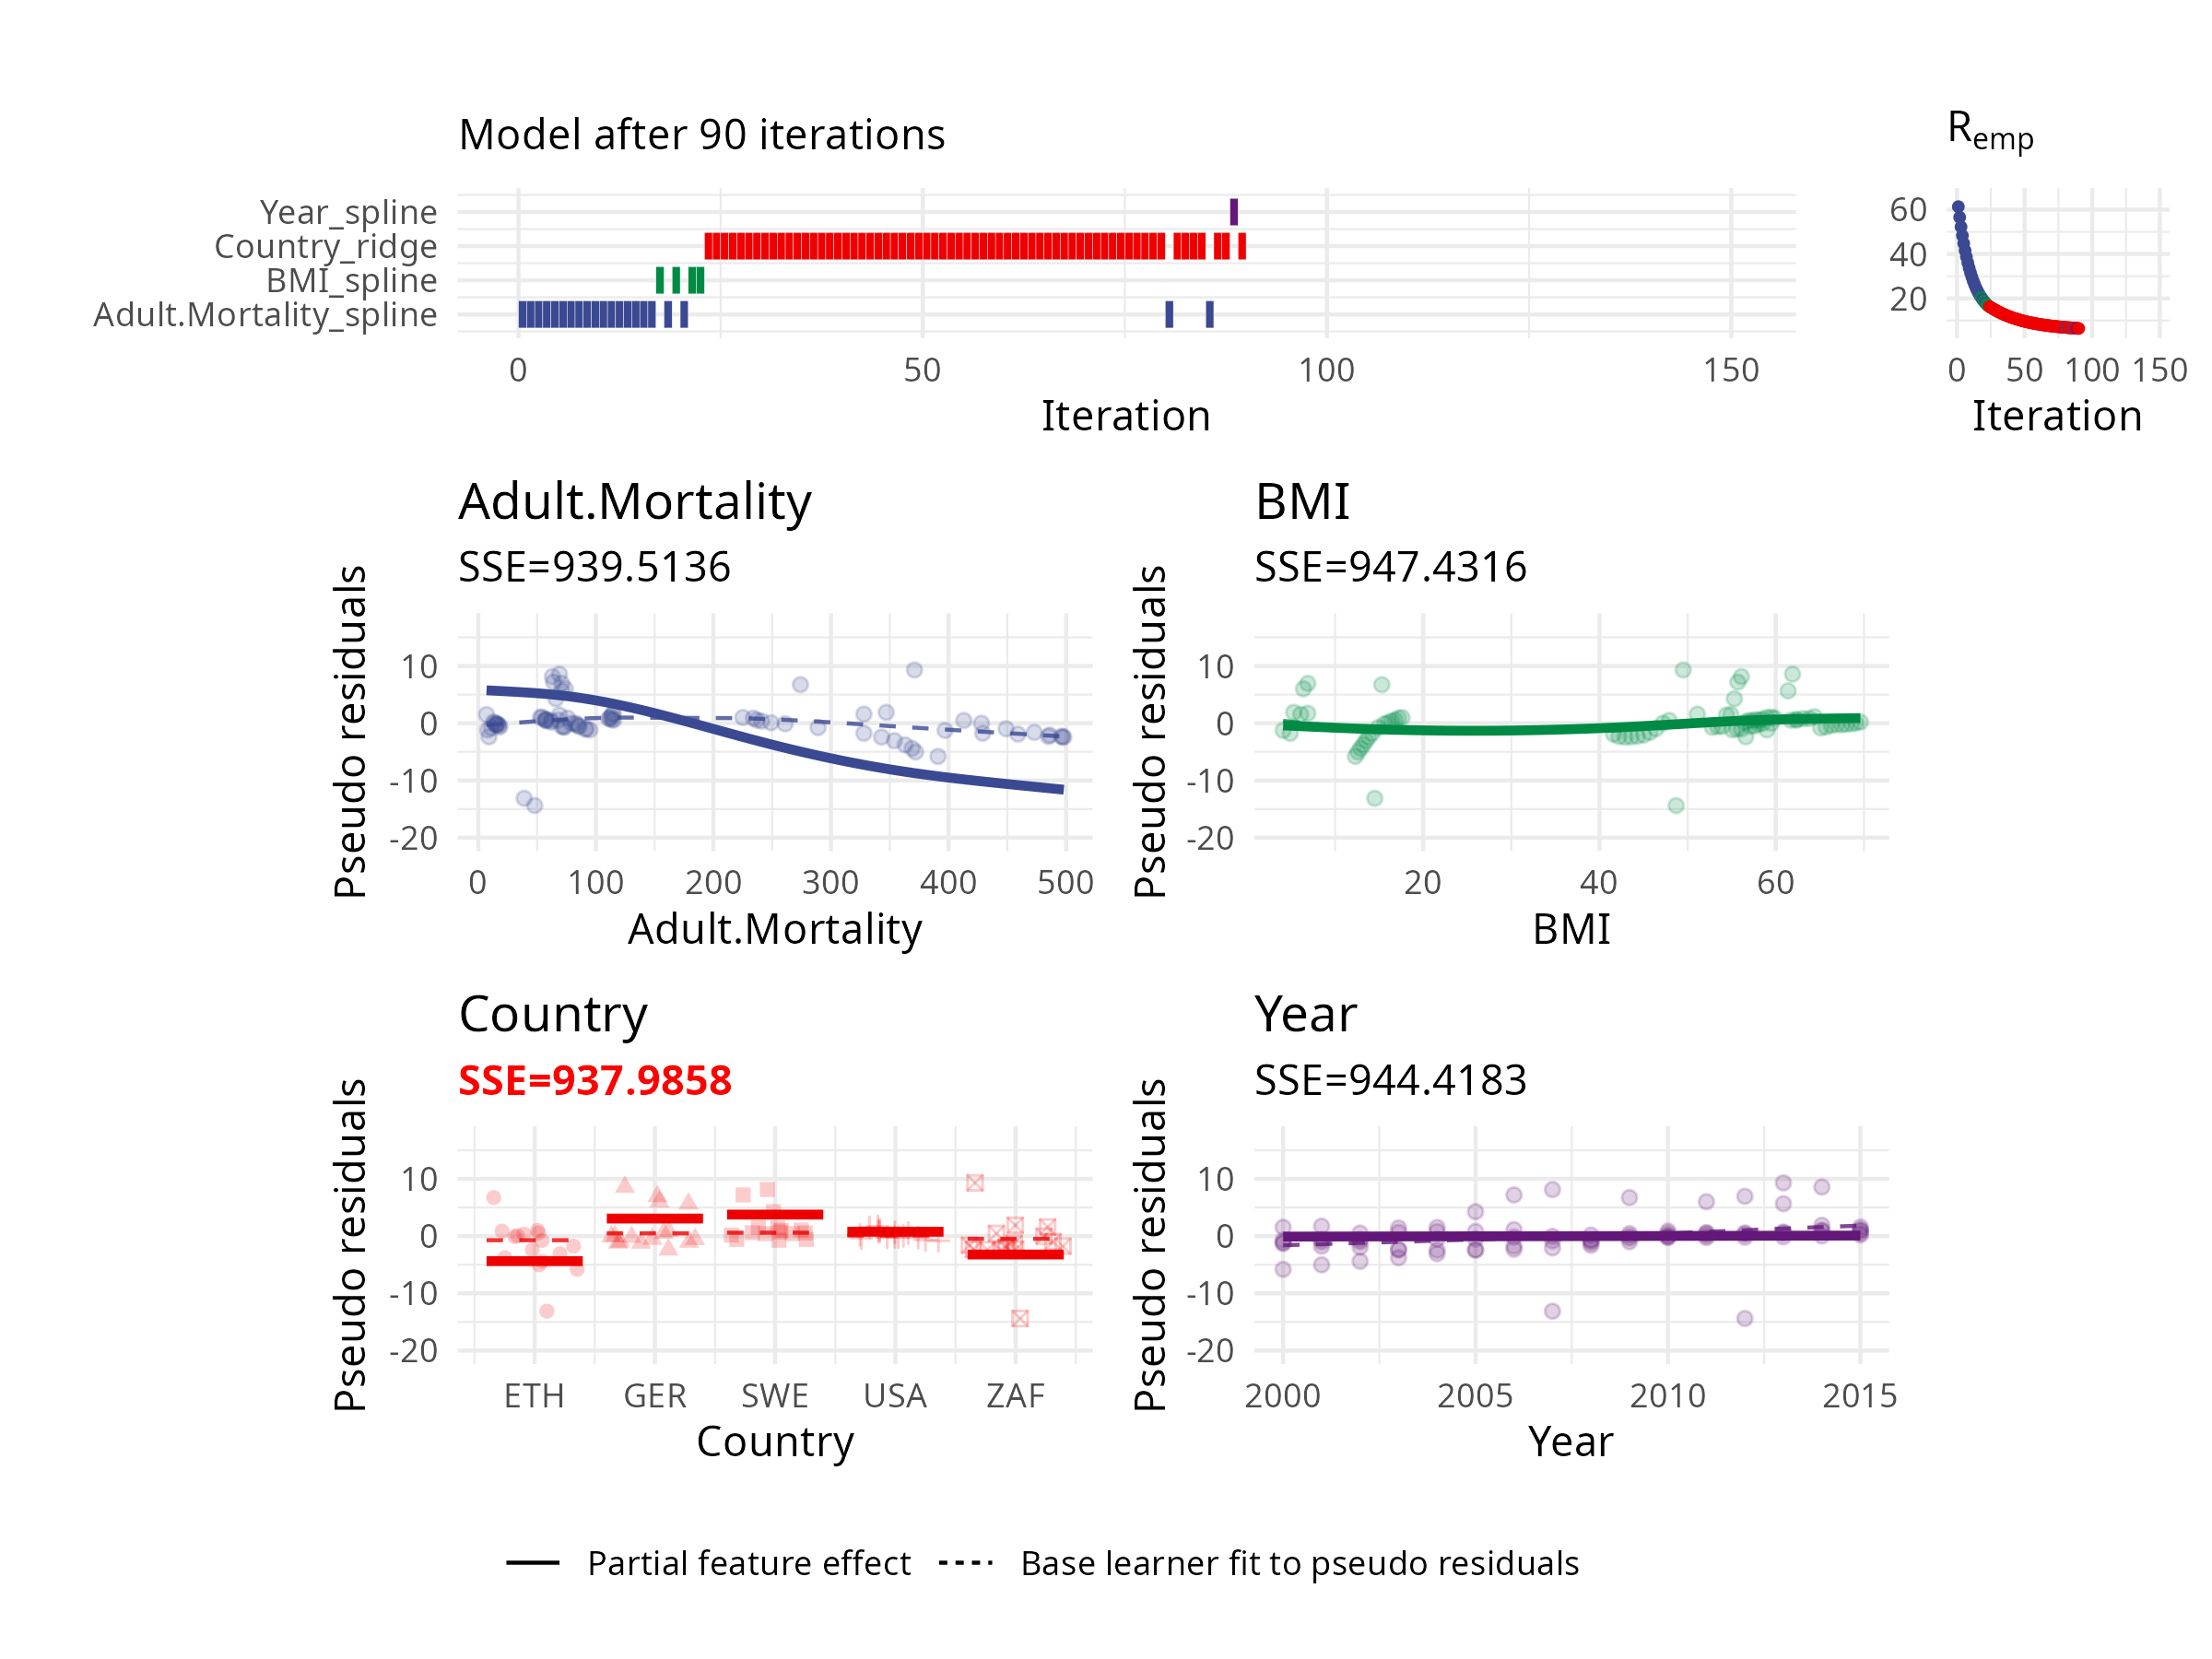
\includegraphics[width=\textwidth]{figures/cwb-anim/fig-iter-0090.png}
	\end{figure}
	\addtocounter{framenumber}{-1}
\end{frame}


\begin{frame}{Example: Life expectancy (nonlinear)}
	\begin{figure}
		\centering
		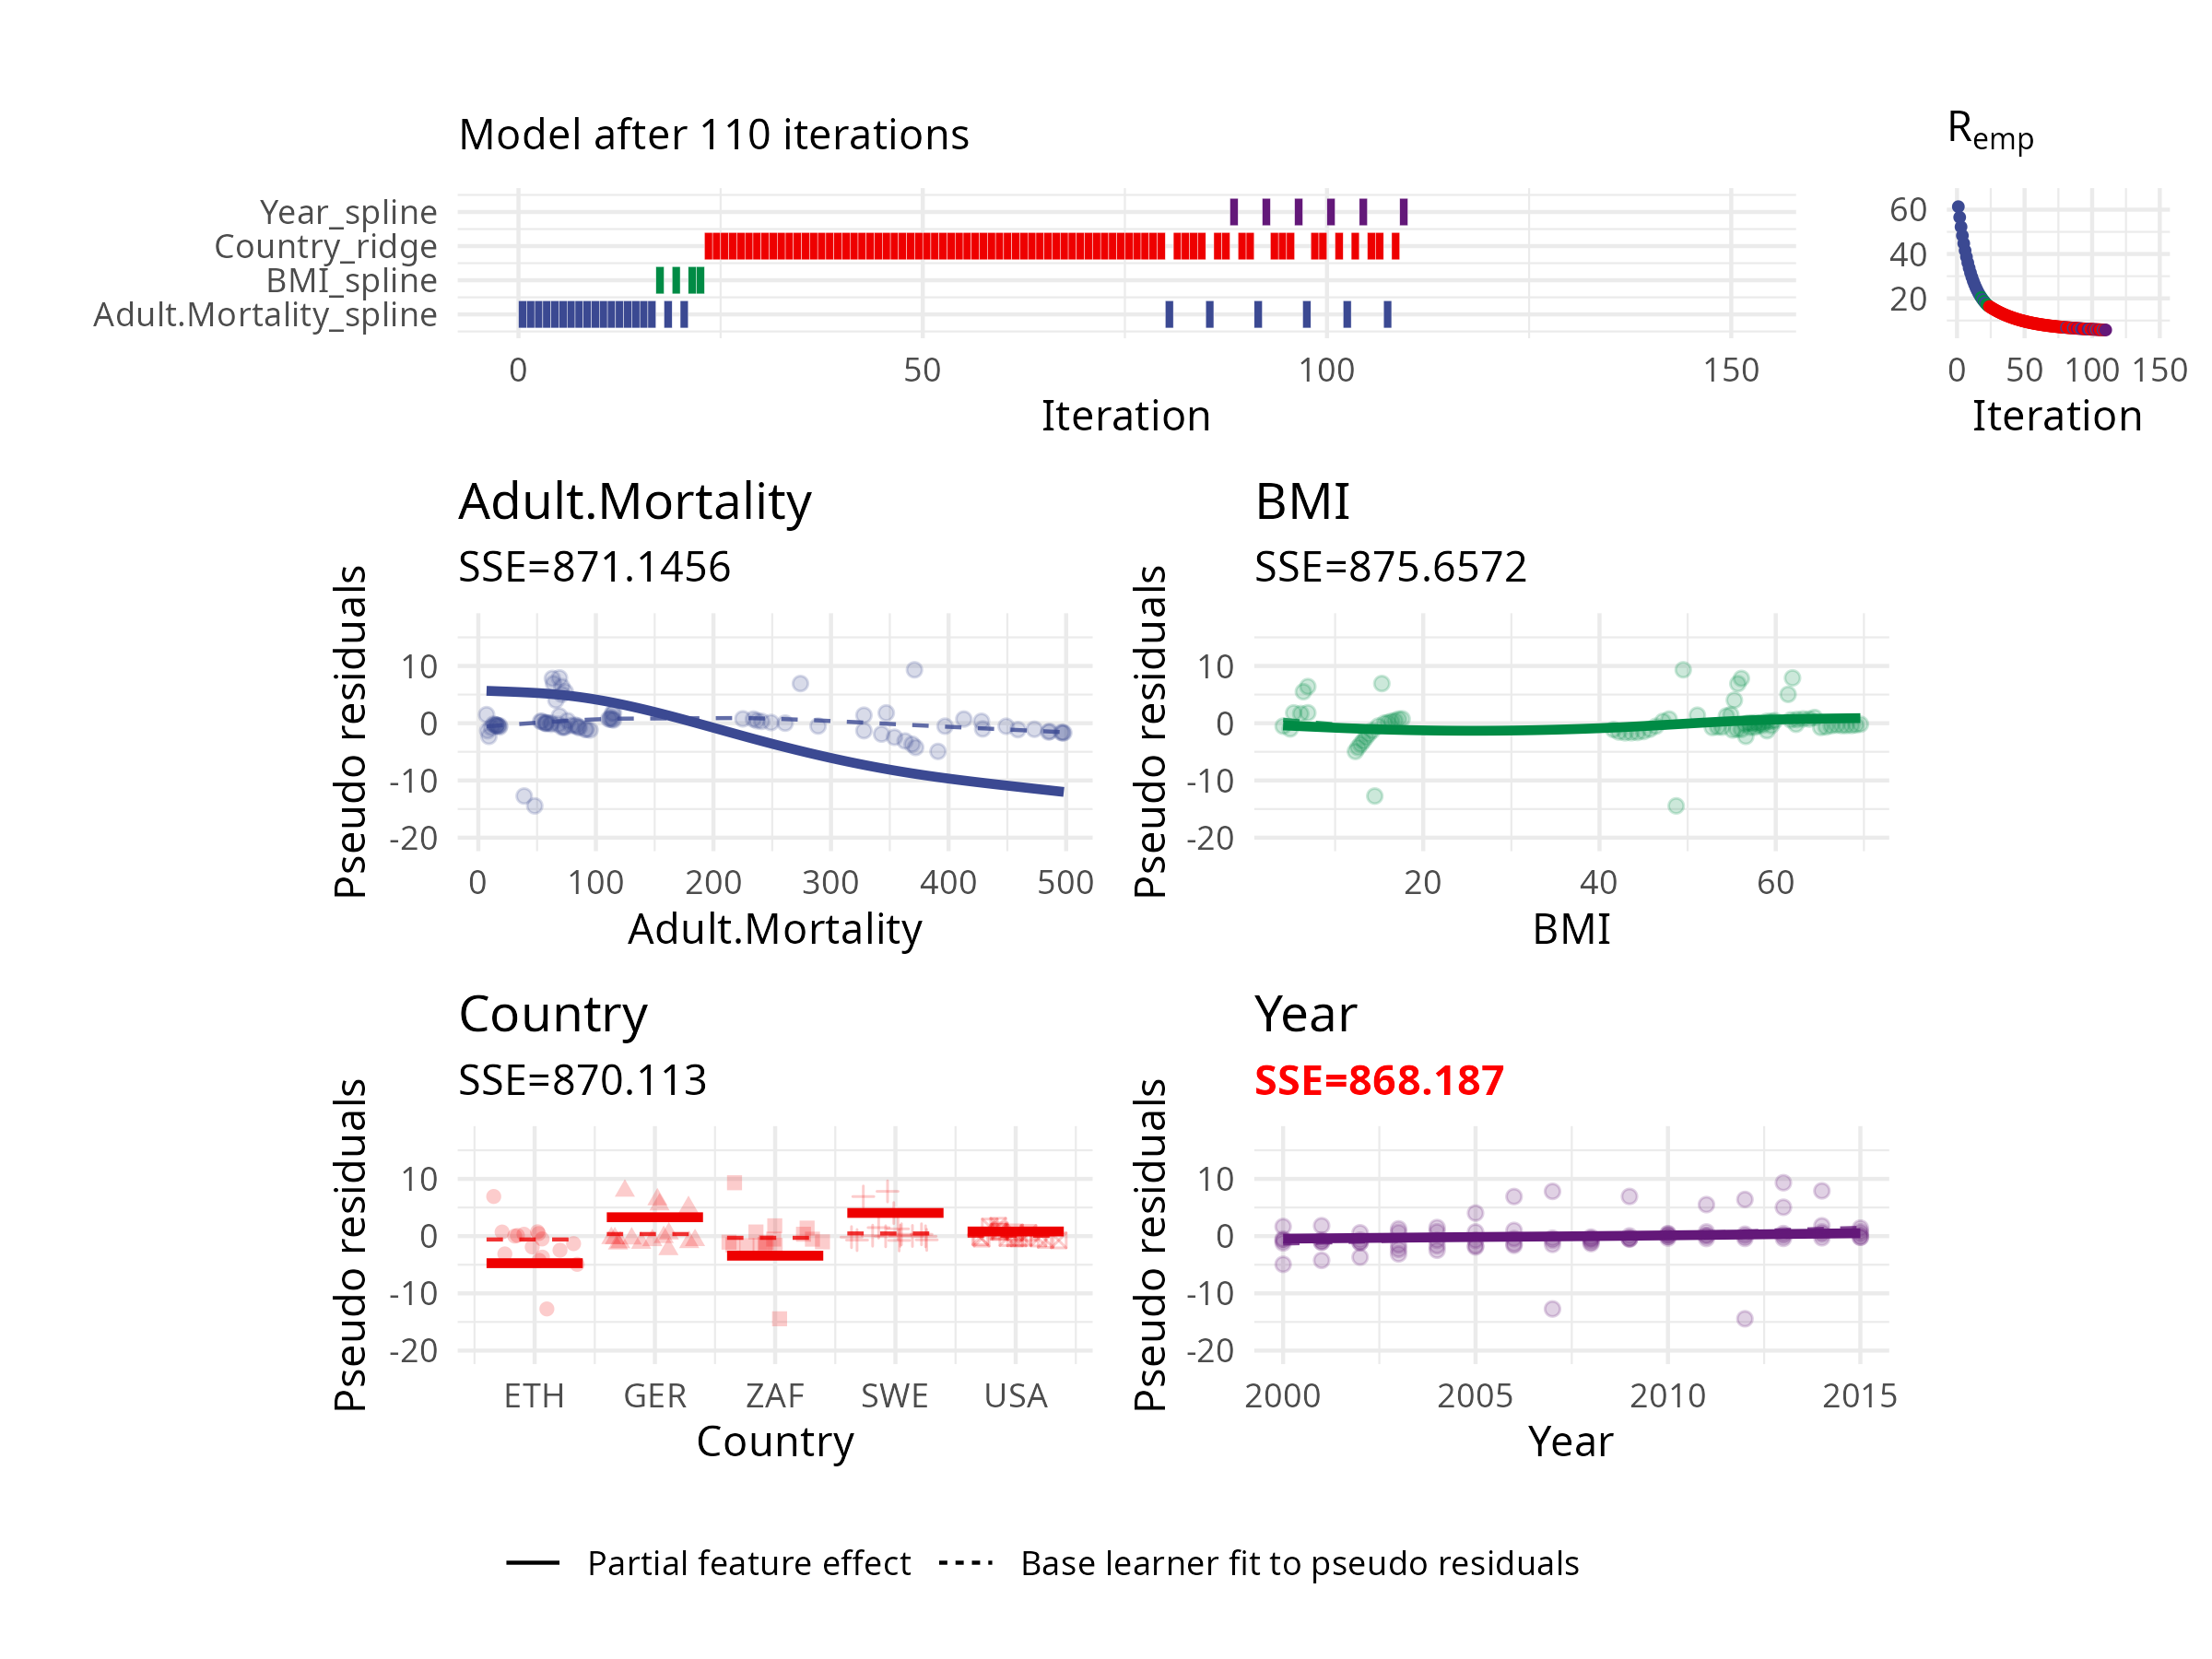
\includegraphics[width=\textwidth]{figures/cwb-anim/fig-iter-0110.png}
	\end{figure}
	\addtocounter{framenumber}{-1}
\end{frame}


\begin{frame}{Example: Life expectancy (nonlinear)}
	\begin{figure}
		\centering
		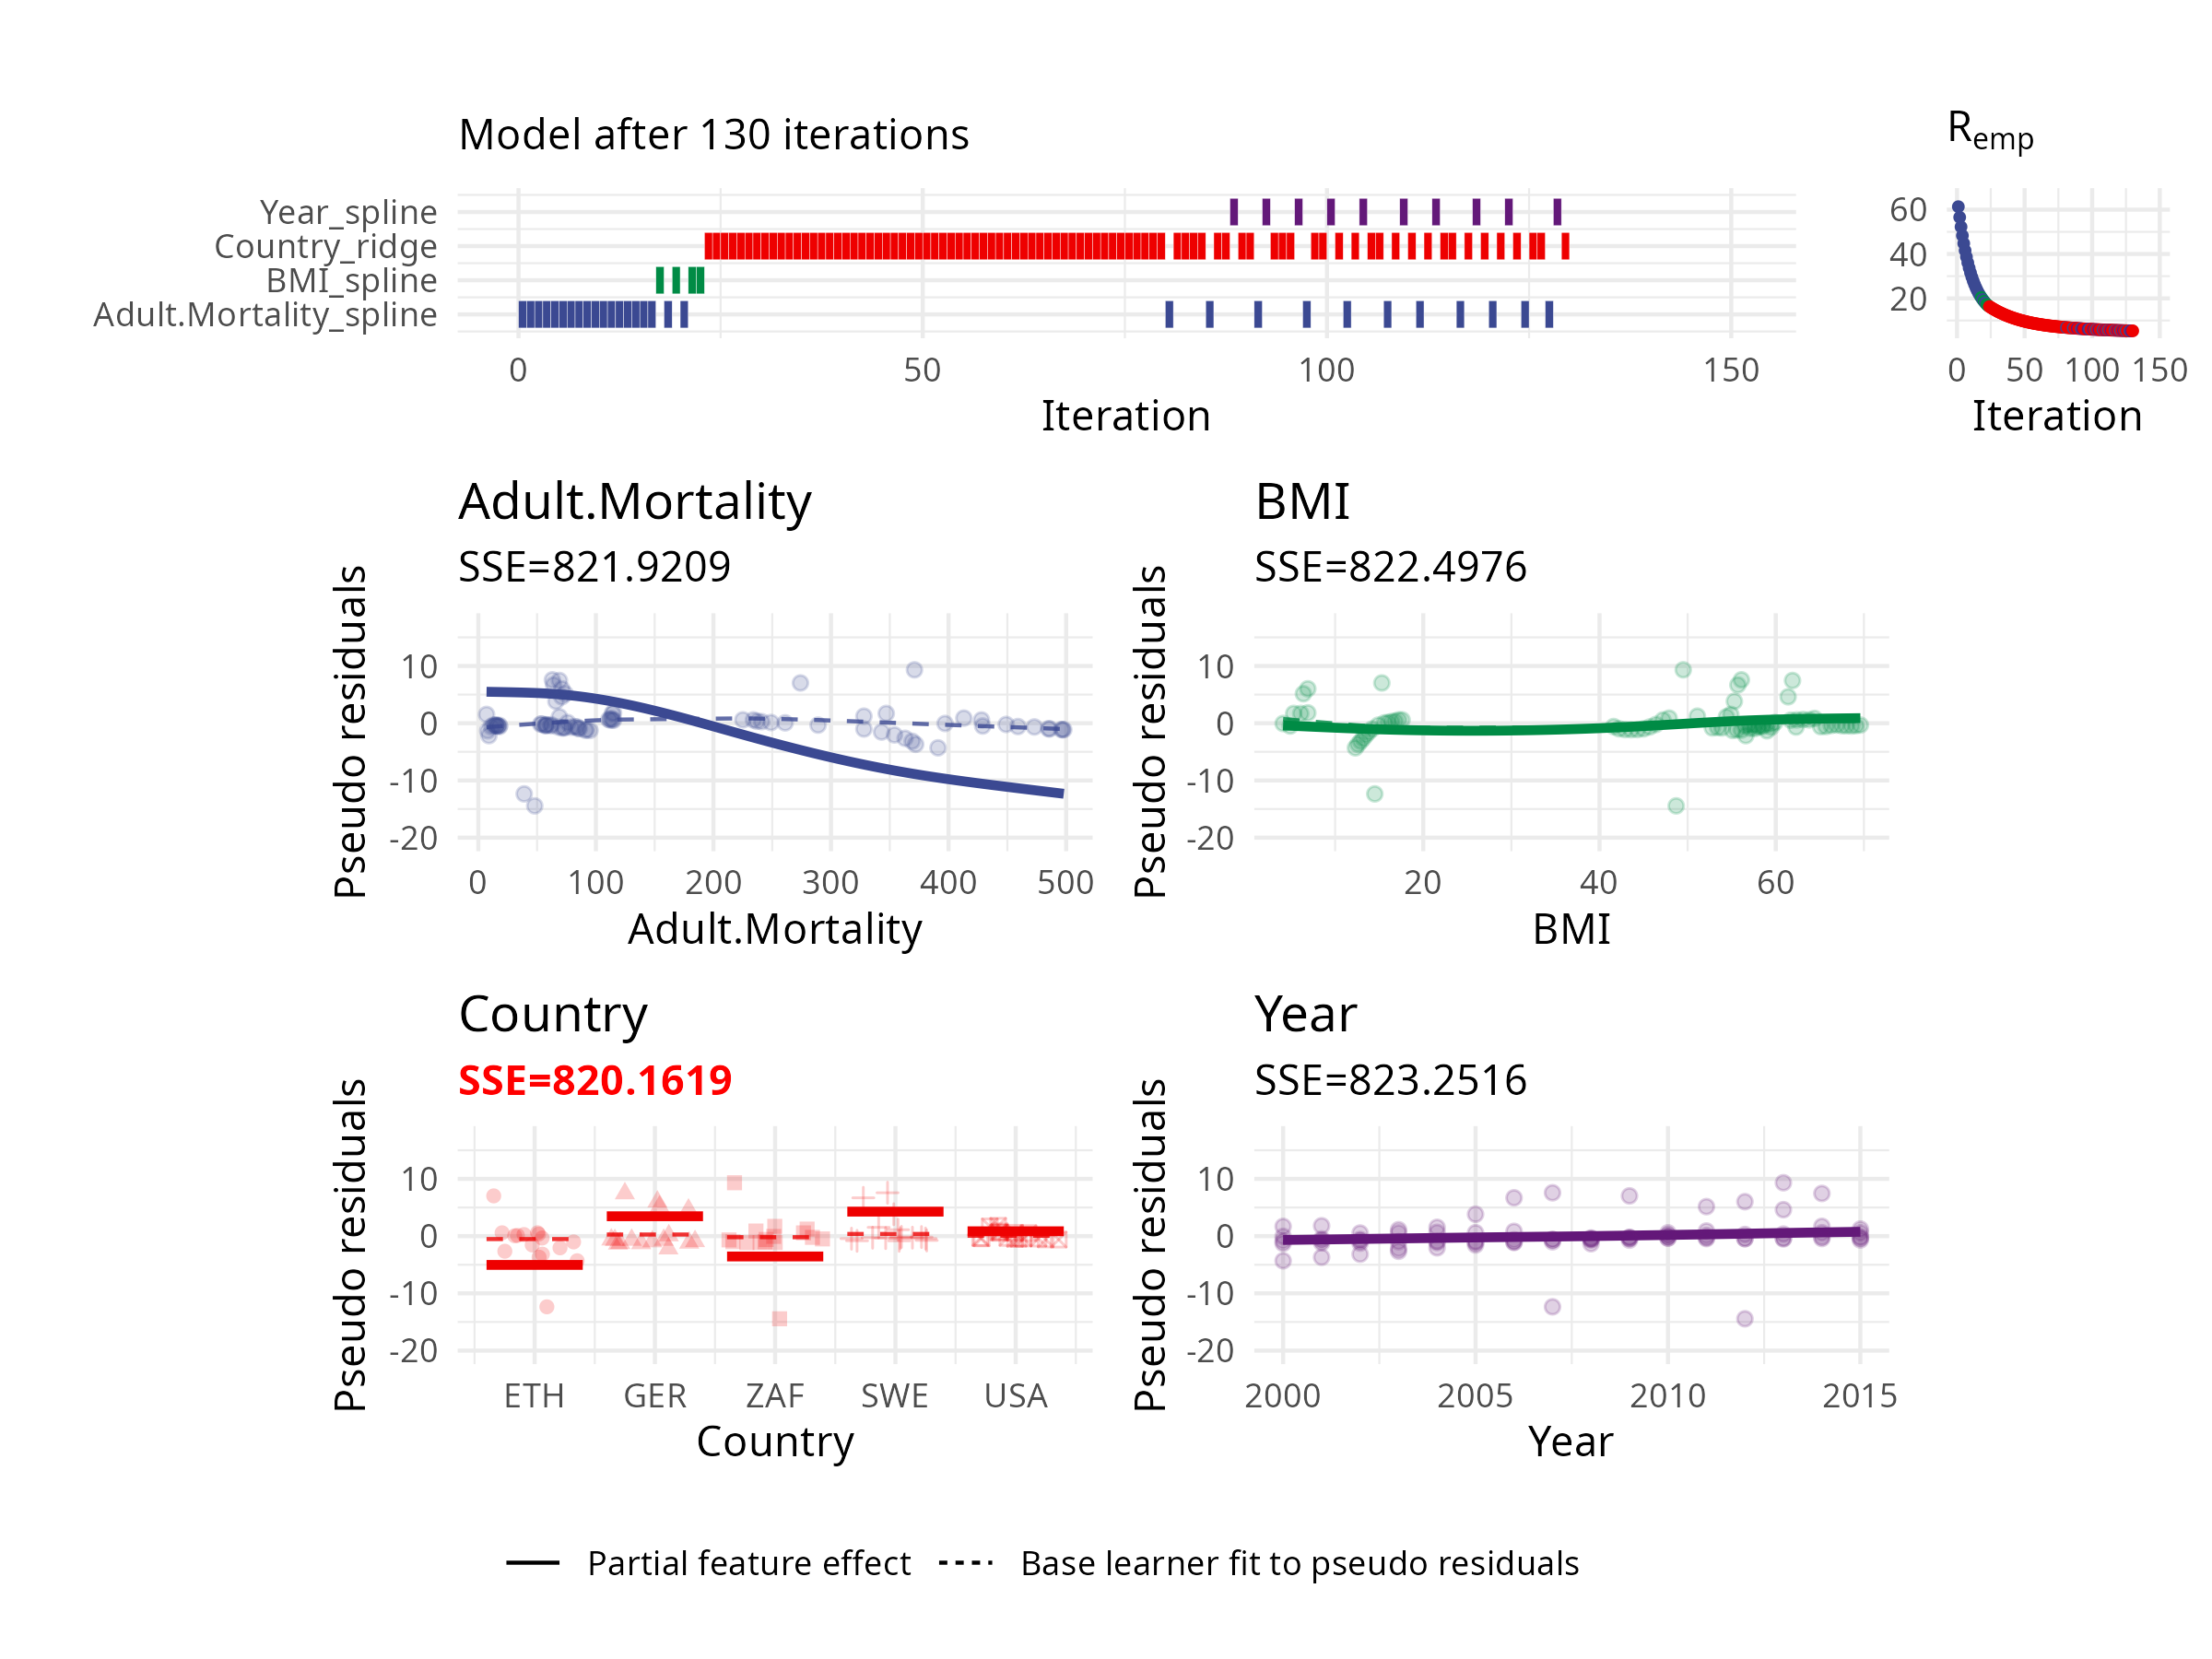
\includegraphics[width=\textwidth]{figures/cwb-anim/fig-iter-0130.png}
	\end{figure}
	\addtocounter{framenumber}{-1}
\end{frame}


\begin{frame}{Example: Life expectancy (nonlinear)}
	\begin{figure}
		\centering
		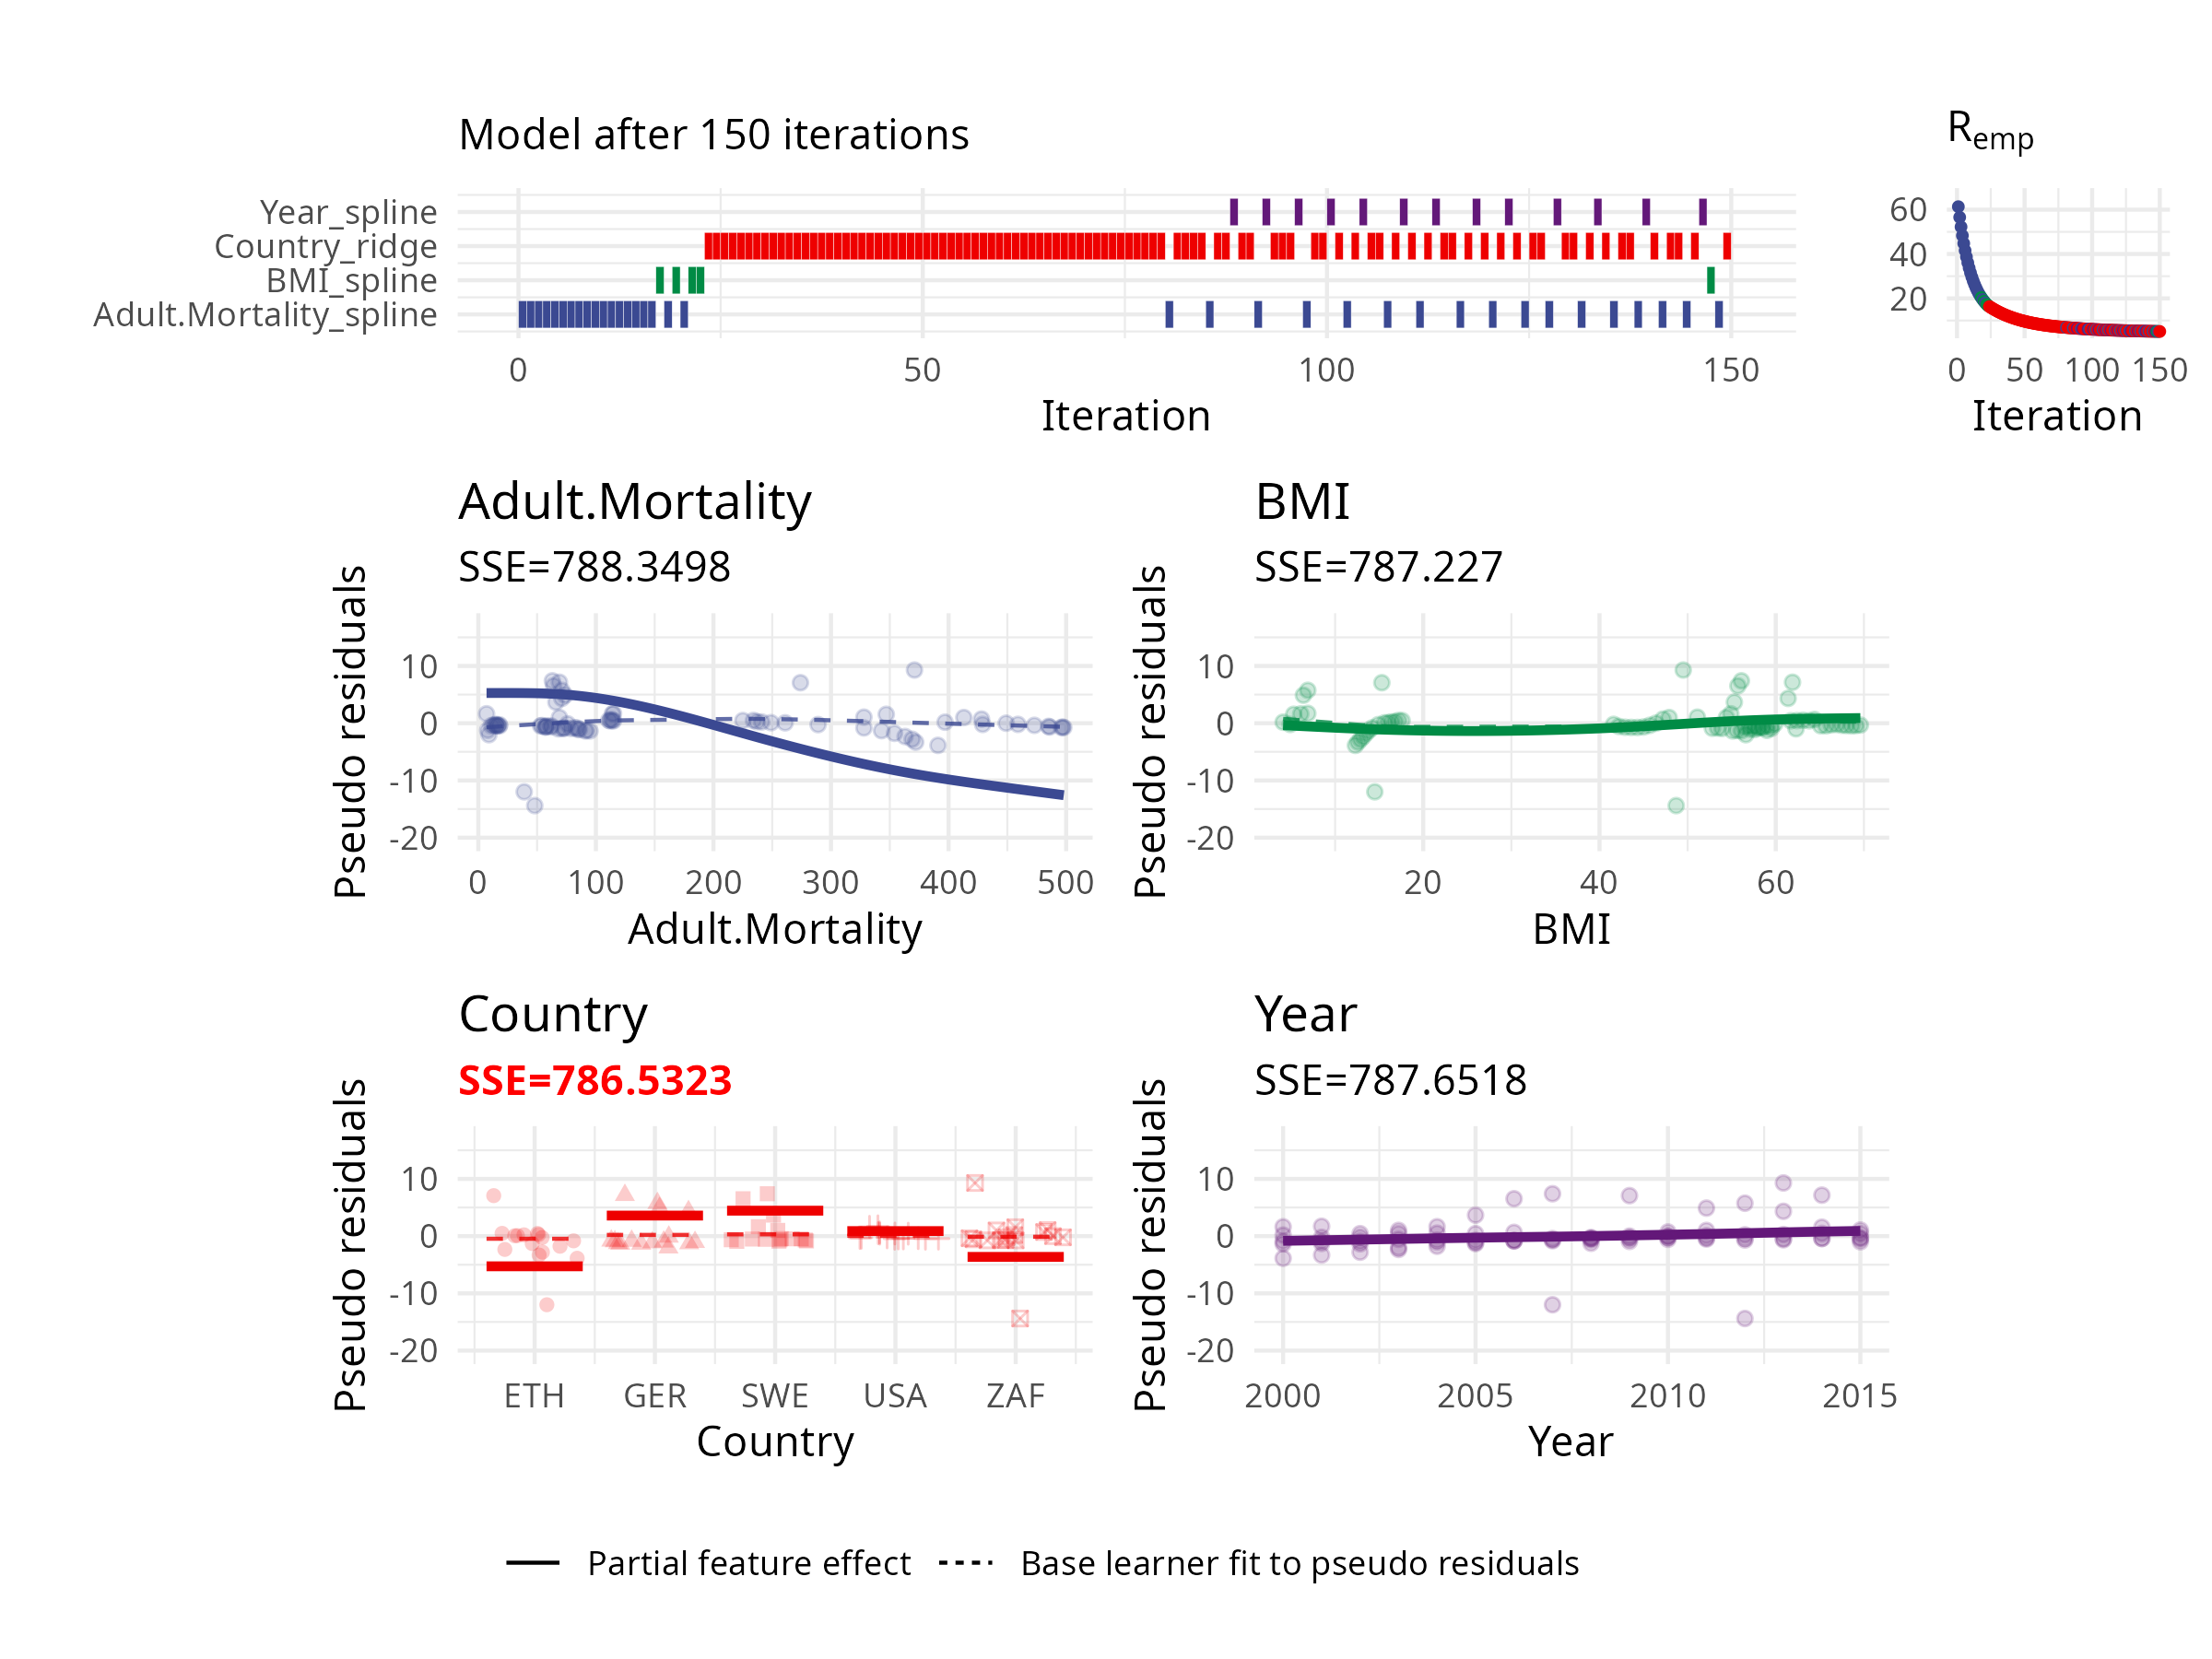
\includegraphics[width=\textwidth]{figures/cwb-anim/fig-iter-0150.png}
	\end{figure}
	\addtocounter{framenumber}{-1}
\end{frame}



\begin{frame}{Component-wise gradient boosting -- Example}
	\begin{figure}
		\centering
		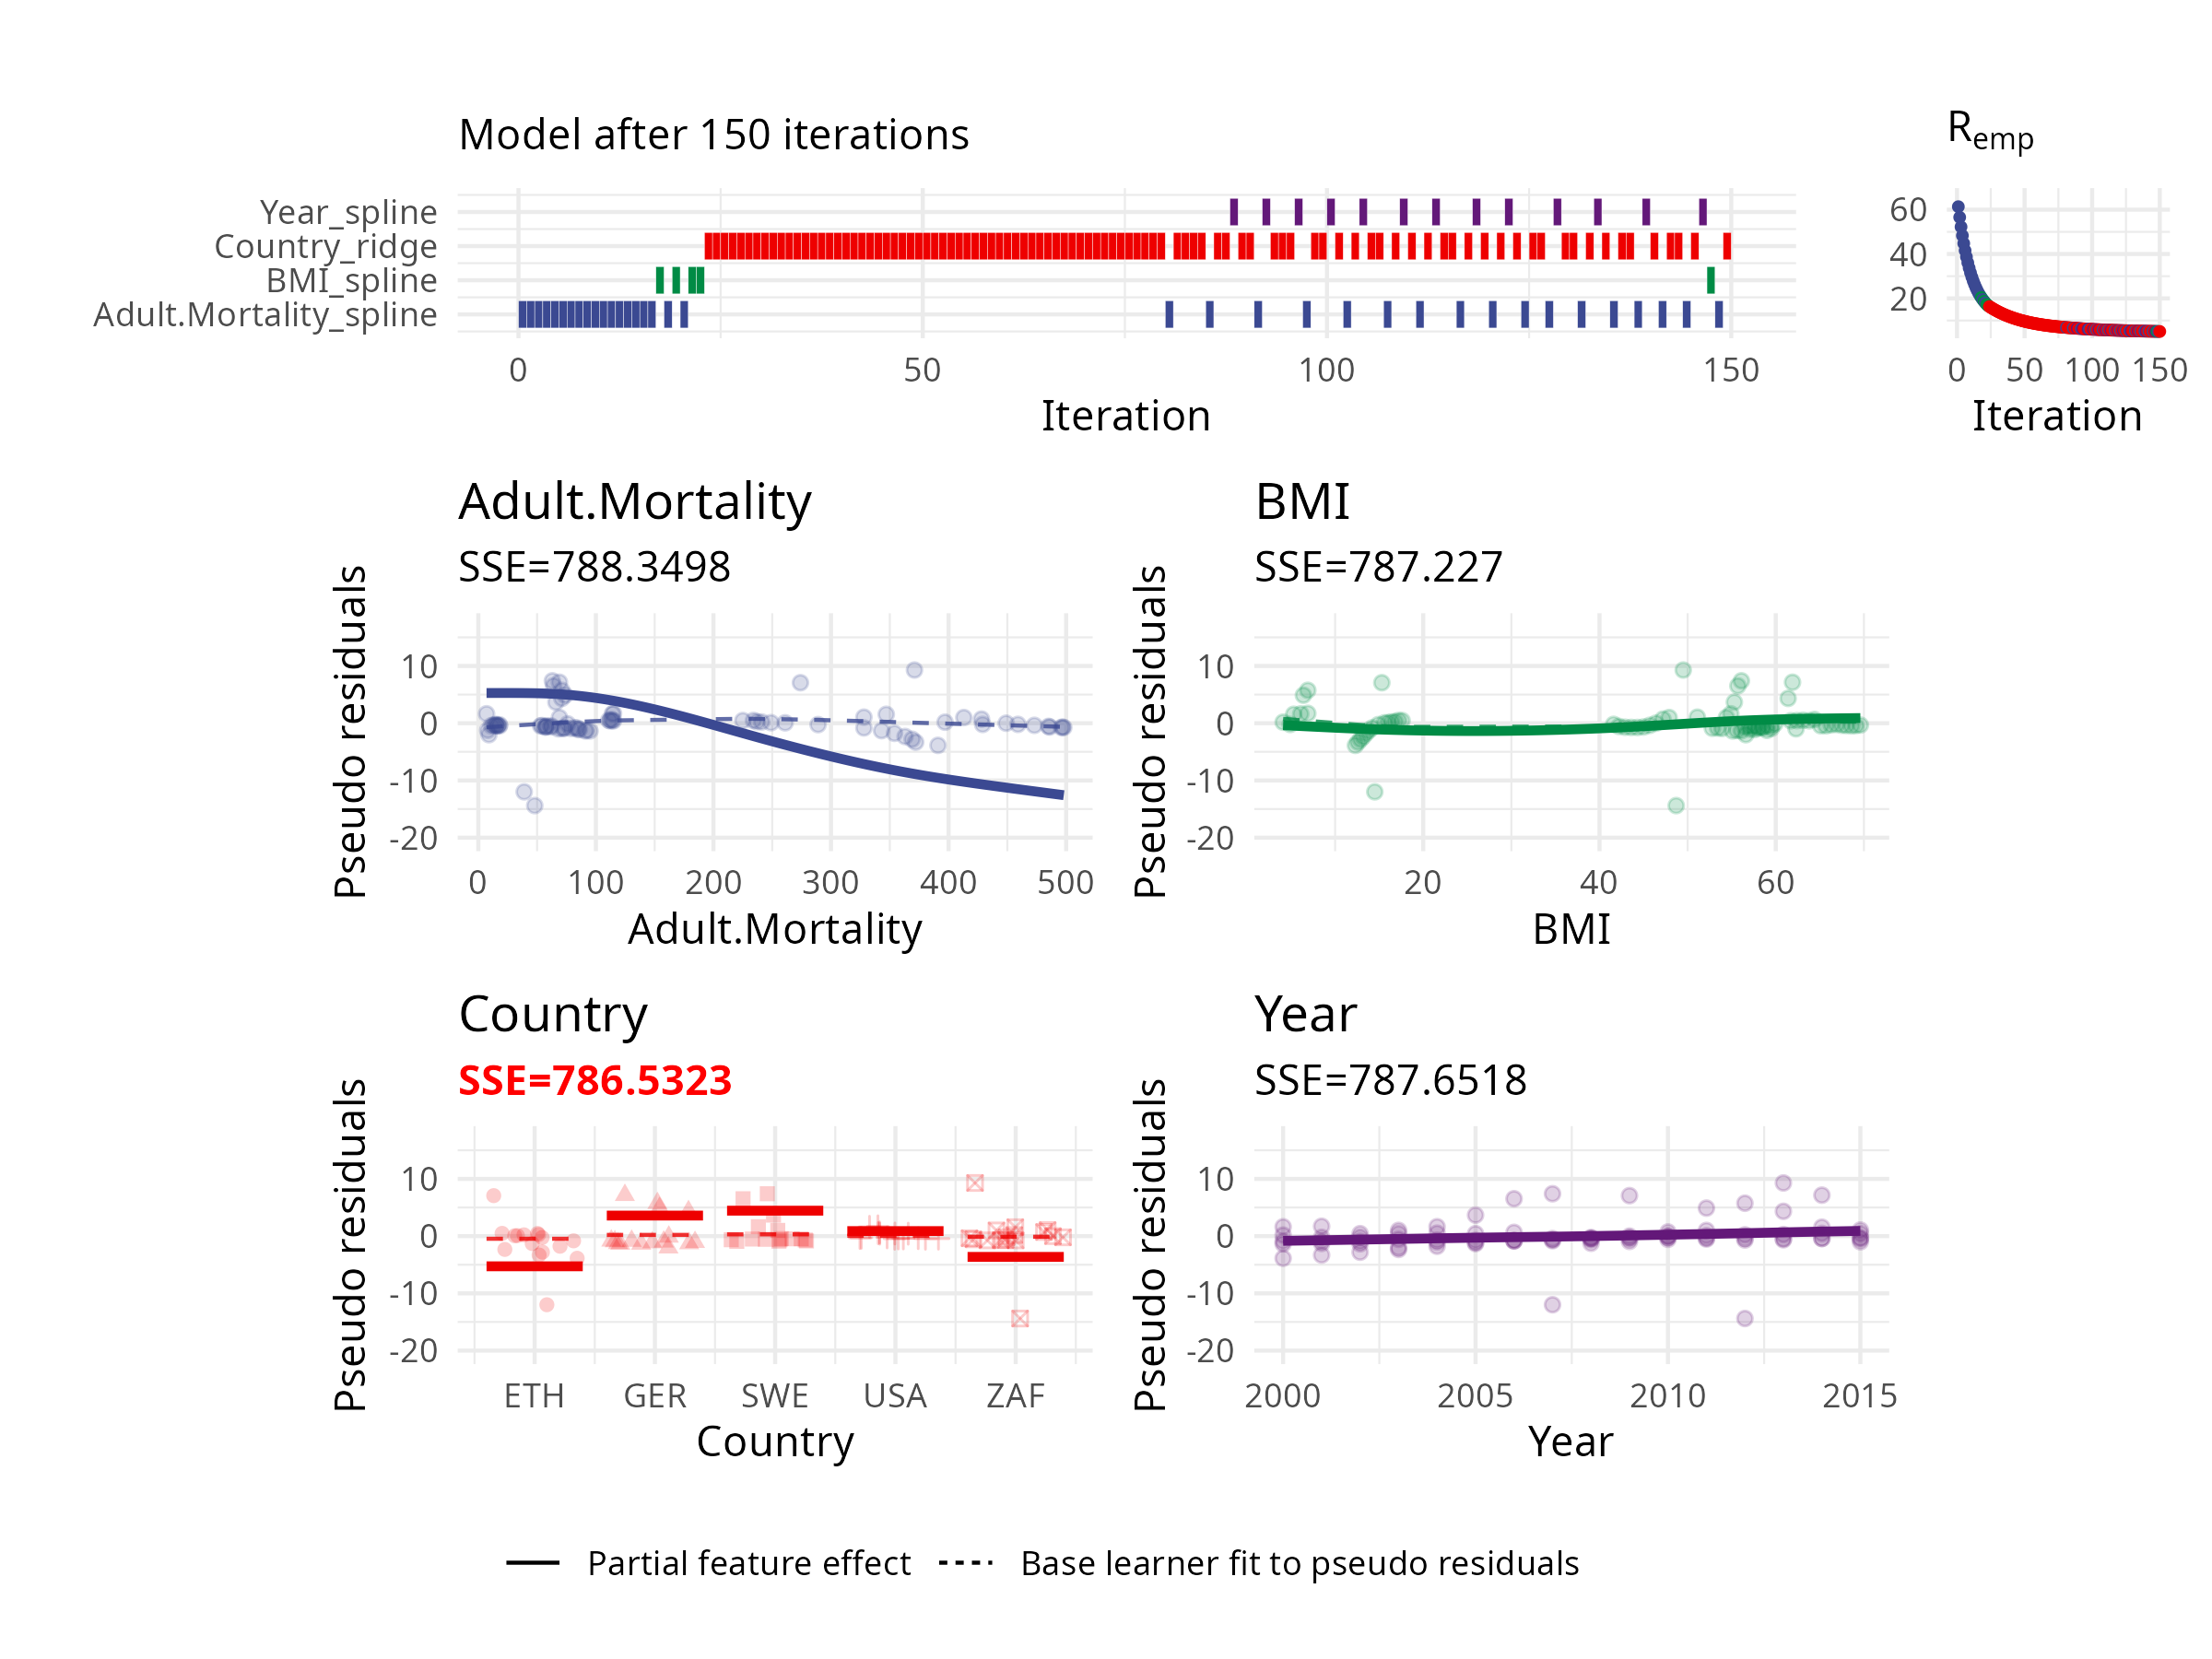
\includegraphics[width=\textwidth]{figures/cwb-anim/fig-iter-0150.png}
	\end{figure}
	\addtocounter{framenumber}{-1}
\end{frame}


\section{Efficiency}

\begin{frame}{About -- Problems of CWB}

  Computational complexity in terms of memory and runtime efficiency.
  \begin{itemize}
    \item \textbf{W.r.t. runtime:}
    \begin{itemize}
      \item Training CWB requires to (theoretically) calculate $(\design_k^\tran \design_k + \bm{K}_\blk)^{-1}\design_k^\tran \rmm$ for all $k = 1, \dots, K$ and $M$ iterations.
      \item The computational load is tremendously reduced by pre-calculating the Cholesky decompositions of $\design_k^\tran \design_k + \bm{K}_\blk$ for all $k$ as iteration independent part and to re-cycle these matrices in each iteration.
      \item Nevertheless, for big $K$ and $M$ this remains very costly and time consuming.
    \end{itemize}
    \item[] $\Rightarrow$ Fitting the algorithm can take too much time.
  \end{itemize}
\end{frame}

\begin{frame}{About -- Problems of CWB}

  Computational complexity in terms of memory and runtime efficiency.
  \begin{itemize}
    \item \textbf{W.r.t. memory:}
    \begin{itemize}
      \item Each base learner requires to store a design matrix.
      \item For example, using B-splines, it is common to to store an $n\times 24$ matrix (with $20$ knots, and cubic basis functions) for one numerical feature.
    \end{itemize}
    \item[] $\Rightarrow$ The RAM is filled very fast.
  \end{itemize}
\end{frame}

\begin{frame}{About -- Problems of CWB}

  Computational complexity in terms of memory and runtime efficiency.
  \begin{itemize}
    \item \textbf{W.r.t. runtime:} Fitting the algorithm can take too much time.
    \item \textbf{W.r.t. memory:} The RAM is filled very fast.
  \end{itemize}
  \begin{itemize}
    \item[$\Rightarrow$] Less attractive or infeasible for medium- to large-scale applications.
  \end{itemize}
\end{frame}

\begin{frame}{About -- Publication}
  %\textbf{Publication:}
  %\renewcommand{\newblock}{\newblocknew}
  %\begin{itemize}
    %\item {\footnotesize\bibentry{schalk2022accelerated}}
  %\end{itemize}
  %\renewcommand{\newblock}{\newblockold}

  \vspace{-0.2cm}
  \begin{figure}
    \centering
    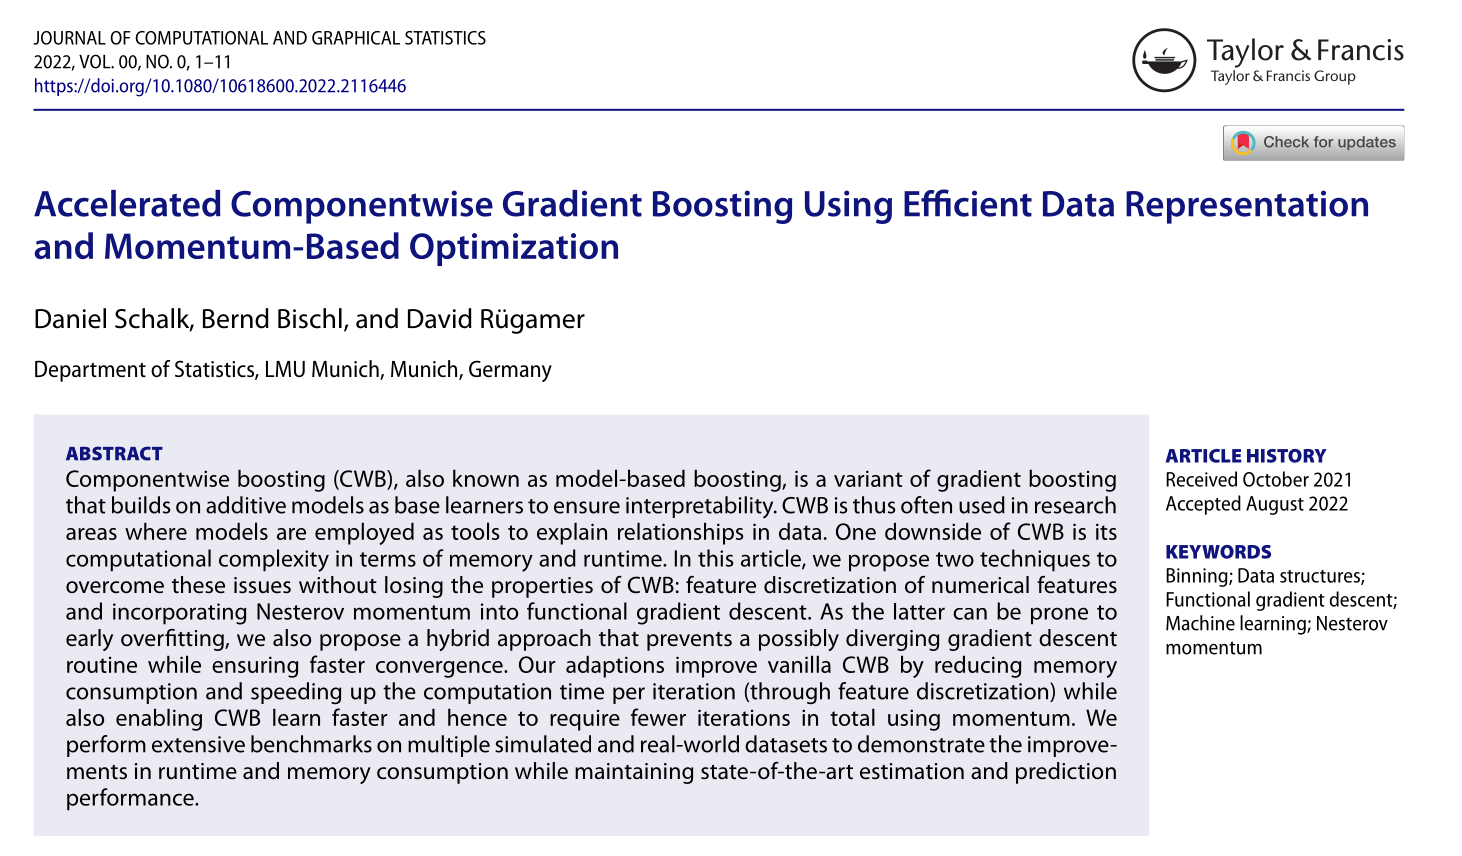
\includegraphics[width=0.7\textwidth]{figures/fig-cacb-paper.png}
  \end{figure}
  \vspace{-0.4cm}

  \textbf{Aims:}
  \begin{itemize}
    \item
      \textbf{Accelerate the fitting process} of CWB by incorporating Nesterovs momentum.
    \item
      \textbf{Reduce the memory load} by implementing a more efficient data representation for the design matrices.
  \end{itemize}

\end{frame}

\begin{frame}[plain]{}
  \Large Efficiency\\[0.3cm]
  {\LARGE\textbf{Accelerating component-wise boosting}}
\end{frame}

\begin{frame}{Accelerating component-wise boosting -- Idea}

  \textbf{Gradient descent:}

  \vspace{0.2cm}
  {\small
  \begin{tabular}{ccc}
    Parameter space & & Function space \\[0.3cm]
    $\tbh^{[m+1]} = \tbh^{[m]} + \nu \nabla_{\tb}\riske(\fh(. | \tbh^{[m]}) | \D)$ & $\Rightarrow$ & $\fh^{[m+1]} = \fmh + \nu \hat{b}^{[m]}$
  \end{tabular}}
  \vspace{0.4cm}

  \textbf{Nesterovs momentum:}

  \vspace{0.2cm}
  {\small
  \begin{tabular}{ccc}
    Parameter space & & Function space \\[0.3cm]
    $\bm{u}^{[m]} = \nabla_{\tb}\riske(\fh(. | \tbh^{[m]} - \gamma \hat{\bm{\vartheta}}^{[m-1]}) | \D)$ &  & \\
    $\hat{\bm{\vartheta}}^{[m]} = \gamma \hat{\bm{\vartheta}}^{[m-1]} + \nu \bm{u}^{[m]}$ & $\Rightarrow$ & ??? \\
    $\tbh^{[m+1]} = \tbh^{[m]} + \hat{\bm{\vartheta}}^{[m]}$ & &
  \end{tabular}}
  \vspace{0.2cm}

  \begin{itemize}
  \item[$\Rightarrow$] \textbf{Idea:} Use Nesterovs momentum and adjust it for functional updates and CWB.
  \end{itemize}

\end{frame}

\begin{frame}{Accelerating component-wise boosting -- Idea}

  \begin{itemize}
    \item
      Using momentum and Nesterovs momentum was first proposed by \cite{biau2019accelerated} and refined in an algorithm called Accelerated Gradient Boosting Machine (AGBM) by \cite{lu2020accelerating}:
      \begin{align*}
      g^{[m]} &= (1 - \theta_m) f^{[m]} + \theta_m h^{[m]}\\
      f^{[m+1]} &= g^{[m]} + \eta b^{[m]} \\
      h^{[m+1]} &= h^{[m]} + \eta / \theta_m b^{[m]}_{\text{cor}}
      \end{align*}
    \item
      Incorporate these adjustments into CWB and make sure all advantages are preserved.
  \end{itemize}
  %\textbf{Memory reduction}
  %\begin{itemize}
    %\item
      %Reduce the memory consumption of CWB
    %\item
      %Apply binning~\citep{} to reduce the matrix size of each base learner and ensure
    %\item
      %Side effect: The runtime also gets better.
  %\end{itemize}

\end{frame}

\begin{frame}{Base learners in AGBM}
  \begin{itemize}
    \item
      \(b^{[m]}\) is fit to pseudo residuals \(\rmm\) w.r.t.
      \(\hat{g}^{[m-1]}\) instead of \(\fmh\)

    \item
      AGBM introduces a second base learner $b^{[m]}_{\text{cor}}$ that is fitted to error-corrected pseudo residuals:
      \[c^{[m](i)} = \rmi + \frac{m}{m+1}(c^{[m-1](i)} - \hat{b}_{\text{cor}}^{[m-1]}(\xi)),\]
      with \(i = 1, \dots, n\), if \(m > 1\) and \(\bm{c}^{[m]} = \rmm\) if
      \(m = 0\).

    \item[] $Rightarrow$ Each iteration adds not one but two base learners $b^{[m]}$ and $b^{[m]}_{\text{cor}}$:
      \begin{itemize}
        \item $b^{[m]}_{\text{cor}}$ defines the momentum sequence to accelerate the fitting into the direction of the error-corrected pseudo residuals
        \item Computing a second base learner also means two double the runtime for the same number of iterations.
      \end{itemize}
  \end{itemize}
\end{frame}


\begin{frame}{Accelerating component-wise boosting}
  \citet{schalk2022accelerated} introduces an accelerated CWB (ACWB)
  version by incorporating these adaptions to CWB, therefore:

  \begin{itemize}
    \item
      Both base learners, \(b^{[m]}\) and \(b^{[m]}_{\text{cor}}\), are the
      result of a selection process that chooses one of \(b_1, \dots, b_K\)
      w.r.t. to the minimal SSE on the respective pseudo residuals \(\rmm\)
      and \(\bm{c}^{[m]}\).
    \item
      Update the estimated parameters accordingly to allow the estimation of
      partial feature effects.
  \end{itemize}
  Considering these points allows to maintain all advantages of CWB in
  ACWB. Details are outlined in the publication.
\end{frame}

\begin{frame}{Hybrid component-wise boosting}
  \begin{itemize}
    \item
      It was proven by \citet{lu2020accelerating}, that ACWB can overfit if
      not stopped early.
    \item
      Therefore, a hybrid CWB (HCWB) approach combines ACWB for an accelerated fitting in the beginning and CWB
      to fine-tune the model:
  \end{itemize}

  \begin{figure}
    \centering
    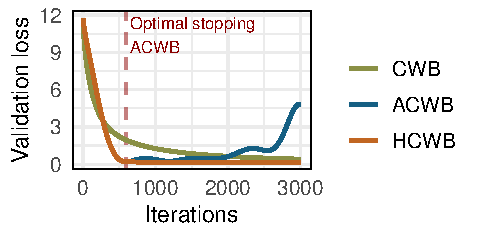
\includegraphics[width=0.7\textwidth]{figures/fig-HCWB.pdf}
  \end{figure}
\end{frame}


\begin{frame}{Results}
  About
\end{frame}

\begin{frame}[plain]{}
  \Large Efficiency\\[0.3cm]
  {\LARGE\textbf{Reduced memory consumption in component-wise boosting}}
\end{frame}

\begin{frame}{Adaption}
  About
\end{frame}

\begin{frame}{Results}
  About
\end{frame}


\section{Automation}

\begin{frame}{Automation}
  About
\end{frame}

\begin{frame}{Autocompboost}
  About
\end{frame}

\begin{frame}{Results}
  About
\end{frame}

\begin{frame}{Outlook}
  About
\end{frame}


\section{Distributed computing}

\begin{frame}{Distributed computing}
  About
\end{frame}

\begin{frame}{Adaption}
  About
\end{frame}

\begin{frame}{Results}
  About
\end{frame}

\begin{frame}{Outlook}
  About
\end{frame}


\begin{frame}[allowframebreaks]{Bla}

  Bla
  \citep[see, e.g.,][]{Pepe2003}, or \cite{delong1988comparing}

\end{frame}

\appendix

\begin{frame}[allowframebreaks]{References}

\nocite{*}
\scriptsize
\bibliography{references}

\end{frame}

\section{Backup slides}

\begin{frame}{Backup}

bla

\end{frame}

\end{document}
